\documentclass[]{elsarticle} %review=doublespace preprint=single 5p=2 column
%%% Begin My package additions %%%%%%%%%%%%%%%%%%%
\usepackage[hyphens]{url}

  \journal{?} % Sets Journal name


\usepackage{lineno} % add
\providecommand{\tightlist}{%
  \setlength{\itemsep}{0pt}\setlength{\parskip}{0pt}}

\usepackage{graphicx}
%%%%%%%%%%%%%%%% end my additions to header

\usepackage[T1]{fontenc}
\usepackage{lmodern}
\usepackage{amssymb,amsmath}
\usepackage{ifxetex,ifluatex}
\usepackage{fixltx2e} % provides \textsubscript
% use upquote if available, for straight quotes in verbatim environments
\IfFileExists{upquote.sty}{\usepackage{upquote}}{}
\ifnum 0\ifxetex 1\fi\ifluatex 1\fi=0 % if pdftex
  \usepackage[utf8]{inputenc}
\else % if luatex or xelatex
  \usepackage{fontspec}
  \ifxetex
    \usepackage{xltxtra,xunicode}
  \fi
  \defaultfontfeatures{Mapping=tex-text,Scale=MatchLowercase}
  \newcommand{\euro}{€}
\fi
% use microtype if available
\IfFileExists{microtype.sty}{\usepackage{microtype}}{}
\usepackage[margin=1.1in]{geometry}
\bibliographystyle{elsarticle-harv}
\usepackage{longtable,booktabs,array}
\usepackage{calc} % for calculating minipage widths
% Correct order of tables after \paragraph or \subparagraph
\usepackage{etoolbox}
\makeatletter
\patchcmd\longtable{\par}{\if@noskipsec\mbox{}\fi\par}{}{}
\makeatother
% Allow footnotes in longtable head/foot
\IfFileExists{footnotehyper.sty}{\usepackage{footnotehyper}}{\usepackage{footnote}}
\makesavenoteenv{longtable}
\ifxetex
  \usepackage[setpagesize=false, % page size defined by xetex
              unicode=false, % unicode breaks when used with xetex
              xetex]{hyperref}
\else
  \usepackage[unicode=true]{hyperref}
\fi
\hypersetup{breaklinks=true,
            bookmarks=true,
            pdfauthor={},
            pdftitle={Spatial variation in predator diel activity patterns -- feral cats avoid red foxes in time, not space},
            colorlinks=false,
            urlcolor=blue,
            linkcolor=magenta,
            pdfborder={0 0 0}}
\urlstyle{same}  % don't use monospace font for urls

\setcounter{secnumdepth}{5}
% Pandoc toggle for numbering sections (defaults to be off)

% Pandoc citation processing

% Pandoc header
\usepackage{setspace}\doublespacing
\usepackage{float}
\floatplacement{figure}{H}
\newcommand{\beginsupplement}{\setcounter{table}{0}  \renewcommand{\thetable}{S\arabic{table}} \setcounter{figure}{0} \renewcommand{\thefigure}{S\arabic{figure}} \setcounter{section}{0} \renewcommand{\thesection}{S\arabic{section}}}
\usepackage{lineno}
\usepackage{booktabs}
\usepackage{longtable}
\usepackage{array}
\usepackage{multirow}
\usepackage{wrapfig}
\usepackage{float}
\usepackage{colortbl}
\usepackage{pdflscape}
\usepackage{tabu}
\usepackage{threeparttable}
\usepackage{threeparttablex}
\usepackage[normalem]{ulem}
\usepackage{makecell}
\usepackage{xcolor}



\begin{document}
\begin{frontmatter}

  \title{Spatial variation in predator diel activity patterns -- feral cats avoid red foxes in time, not space}
    \author[UOM]{Matthew W. Rees\corref{1}}
   \ead{matt.wayne.rees@gmail.com} 
    \author[CEC]{Jack H. Pascoe}
  
    \author[CEC]{Mark Le Pla}
  
    \author[ARI]{Alan Robley}
  
    \author[CEC]{Emma K. Birnbaum}
  
    \author[UOM]{Brendan A. Wintle}
  
    \author[UOM]{Bronwyn A. Hradsky}
  
      \address[UOM]{Quantitative \& Applied Ecology Group, School of Ecosystem and Forest Science, The University of Melbourne, Parkville, VIC, Australia}
    \address[CEC]{Conservation Ecology Centre, Otway Lighthouse Rd, Cape Otway, VIC, Australia}
    \address[ARI]{Department of Environment, Land, Water and Planning, Arthur Rylah Institute for Environmental Research, Heidelberg, Australia}
      \cortext[1]{Corresponding Author}
  
  \begin{abstract}
  
  \end{abstract}
   \begin{keyword} feral cat; diel activity patterns; generalised additive model; invasive predator; intraguild predator interactions; mesopredator release; red fox; lethal predator control\end{keyword}
 \end{frontmatter}

\parskip=12pt

\emph{Article type}: Research Article

\emph{Running title}: Spatiotemporal predator activity

\emph{Word count (abstract, body)}: 330, 4338

\emph{References}: ?

\emph{Figures}: 5

\emph{Tables}: 0

\emph{Authorship}:

\emph{Data accessibility}: Data and code will be deposited on the Dryad Digital Repository after acceptance and can be viewed here: \url{https://github.com/matt-w-rees/spatiotemporal-gams-invasive-predators}.

\newpage

\linenumbers

\hypertarget{abstract}{%
\section*{ABSTRACT}\label{abstract}}
\addcontentsline{toc}{section}{ABSTRACT}

Understanding the constraints that apex predators impose on subordinate species is important for anticipating the outcomes of predator management. Subordinate predators may avoid dominant predators in time or space, making it difficult to quantify changes in antipredator behaviours unless joint spatiotemporal analyses are used.

In this study, we tested whether an invasive apex predator (red fox \emph{Vulpes vulpes}) suppresses or alters the spatiotemporal activity of an invasive mesopredator (feral cat \emph{Felis catus}). We surveyed these predators using 3667 camera-trap deployments across two regions of south-eastern Australia; foxes were poison-baited in some landscapes within each region. The simple predator guild in these regions allowed sharp focus on the interactions between these species across experimental gradients of fox (apex predator) activity. We used generalised additive models to quantify overall predator activity across space and fluctuations in predator activity throughout the daily cycle (i.e., diel activity patterns).

When averaged across the study region, red foxes and feral cats had very similar diel activity patterns; however, there was important differentiation at a finer scale. When fox counts at a camera-trap were high, feral cats did not reduce their overall activity but shifted their diel activity patterns to less risky times of the day. In dry habitats of both regions, cats shifted from being nocturnal-crepuscular to mostly diurnal. In wet forest habitat, fox activity was consistent throughout the diel period; but when fox counts were high, cats became more nocturnal, avoiding dawn in particular. Changes in cat diel activity patterns may facilitate spatial coexistence between the two invasive predators, potentially shifting impacts onto different native prey species.

It is well-appreciated that overall predator activity varies spatially and fluctuates throughout the daily cycle. Our study demonstrates that diel activity patterns also vary across space, likely mediated by both landscape context and fear. Apex predator avoidance appears to be dynamic across landscapes of fear---a key nuance which is overlooked when simply comparing the average activity overlap between two species or the spatial overlap of species occurrence.

\newpage

\hypertarget{introduction}{%
\section{INTRODUCTION}\label{introduction}}

Predators shape ecosystems through both predation and the fear of predation (Creel \& Christianson 2008; Ritchie \& Johnson 2009). Fear-induced behavioural suppression can be as detrimental to subordinate species as predation itself (Schmitz, Krivan, \& Ovadia 2004; Preisser, Bolnick, \& Benard 2005). These non-consumptive effects of apex predator are expected to be strong drivers of mesopredator behaviour, particularly when resource competition is high (Ritchie \& Johnson 2009). A strengthening or relaxing of antipredator behaviours by mesopredators can have cascading effects across the entire ecosystem: altering population demographics, species interactions, ecological function and human-wildlife coexistence (Brown, Laundré, \& Gurung 1999; Ripple \& Beschta 2004; Estes \emph{et al.} 2011; Gaynor \emph{et al.} 2019; Lamb \emph{et al.} 2020). Hence, understanding how apex predators constrain the behaviour of subordinate species is important to accurately predict the ecosystem-wide consequences of predator management, such as reintroductions or lethal control (Gaynor \emph{et al.} 2021).

Spatial and/or temporal niche partitioning may allow predators to coexist by reducing encounter-rates and resource overlap (Kronfeld-Schor \& Dayan 2003). However, mesopredators may not consistently employ avoidance behaviours because perceived predation risk is temporally and spatially variable, and antipredator behaviours typically involve a trade-off against resource acquisition, such as limiting or relegating activity to suboptimal places or times (Lima \& Dill 1990; Lima \& Bednekoff 1999). Therefore, optimal predator avoidance strategies are likely to vary across heterogeneous landscapes where resource availability (e.g., shelter, food) and perceived predation risks differ (Kauffman \emph{et al.} 2007; Willems \& Hill 2009; Wirsing \emph{et al.} 2021). For example, temporal predator avoidance may be preferable over spatial avoidance if food is constantly available throughout the day, and vice versa. These concepts are unified under the `ecology of fear' (Brown, Laundré, \& Gurung 1999) concept, which has gained increasing attention in recent times (Gaynor \emph{et al.} 2019). Notably, the mesopredator release hypothesis has recently been expanded from increases in mesopredator abundance following apex predator decline (Soulé \emph{et al.} 1988) to also include changes in mesopredator behaviour (Brashares \emph{et al.} 2010).

To accurately quantify avoidance within a predator guild, we first need to understand how the overall activity and diel activity patterns of each species varies `naturally' across landscapes, particularly for species with broad distributions. It is widely recognised that the overall activity of different predator species varies across their distributions, but their diel activity patterns are often assumed to be constant. In this paper, we use the term `overall activity' to refer to the number of `independent' predator detections at a site (offset to account for survey duration; analogous to an activity or abundance index), and `diel activity pattern' to refer to fluctuations in relative activity throughout the 24-hour daily cycle. Overall activity is influenced by predator behaviour, population density and the detection process (Anderson 2001), whereas diel activity patterns are a behavioural trait (less likely to be affected by the detection process, if the survey methodology remains consistent).

Despite modern predator survey technologies providing time-stamped detections, detection times are commonly discarded from analyses, probably because joint modelling of overall activity and diel activity patterns is more complicated. When temporal avoidance is tested, it is usually considered in an ad-hoc fashion, by fitting separate models for spatial and temporal avoidance, or by repeating spatial analyses (e.g., resource selection functions) at different time periods (e.g., Smith \emph{et al.} 2019; Basille \emph{et al.} 2015; Kohl \emph{et al.} 2019). However, discretising the daily cycle into categorical periods (e.g., day and night) introduces bias, assuming animals have complete step-changes in behaviour rather than progressive shifts across the daily cycle. Further, dawn and dusk are particularly important times for many predator species.

Generalised Additive Models (hereafter `GAMs') are increasingly being used to estimate animal diel activity patterns and offer a flexible framework to jointly consider overall activity. GAMs also have other benefits, including smoothing penalties to reduce overfitting, the ability to capture nonlinear interactions between multiple variables with different units, and the ability to share information across categorical variables through hierarchical specifications (Wood 2017; Pedersen \emph{et al.} 2019). However, we are only aware of one study which allowed animal diel activity to interact with predation risk as a continuous variable in a GAM (although without considering overall activity; Cunningham \emph{et al.} 2019).

The red fox \emph{Vulpes vulpes} (hereafter `fox'; \textasciitilde6 kg) and feral cat \emph{Felis catus} (hereafter `cat'; \textasciitilde4 kg) have devastating impacts on native prey throughout their introduced range, implicated in the extinction of \textasciitilde10 and 63 species, respectively (Doherty \emph{et al.} 2016). The impacts of these invasive predators have been particularly extreme on the Australian continent (Woinarski, Burbidge, \& Harrison 2015). Cats are more difficult to manage, and so introduced predator control programs in Australia often target only foxes (particularly through poison-baiting; Reddiex \emph{et al.} 2007). As foxes and cats compete for many of the same resources, there is concern that lethal fox control could cause a mesopredator release (Soulé \emph{et al.} 1988) of feral cats (Glen \& Dickman 2005; Robley \emph{et al.} 2014; Marlow \emph{et al.} 2015; Doherty \& Ritchie 2017; Comer \emph{et al.} 2020; Wayne \emph{et al.} 2017). There is some evidence that feral cats increase in activity (although highly uncertain; Hunter \emph{et al.} 2018), density (Chapter \ref{density}) and alter their diets and use of space (Chapter \ref{density}; Molsher \emph{et al.} 2017) in response to fox control. Other studies have investigated potential spatial and temporal interactions between these invasive predators (e.g., Roshier \& Carter 2021), but not in response to fox control, or in a joint spatiotemporal framework that allows flexibility in cat avoidance behaviours in respect to differences in fox activity.

In this study, we explored how the overall activity and diel activity patterns of two competing invasive predators varied across heterogeneous landscapes, in response to (1) space and (2) vegetation types. We then investigated (3) whether cat diel activity patterns change in response to the overall level of fox activity. Our study was conducted in a simple predator system where foxes and cats are the only mammalian carnivores, and fox activity is manipulated using lethal control in some landscapes. This allowed sole focus on the interactions between these two predators, across an experimental gradient of apex predator (fox) activity. We illustrate how GAMs can provide a simple framework to jointly assess spatial and temporal animal activity patterns, as well as avoidance behaviours.

\newpage

\hypertarget{materials-and-methods}{%
\section{MATERIALS AND METHODS}\label{materials-and-methods}}

\hypertarget{study-area-and-camera-trapping}{%
\subsection{Study area and camera-trapping}\label{study-area-and-camera-trapping}}

We compiled data from multiple smaller-scale camera-trap studies across two regions in south-west Victoria, Australia: the Glenelg region and Otway Ranges (Fig. \ref{fig:diel-map}). Introduced foxes and cats are the only medium-large functional mammalian terrestrial carnivores here: native dingoes \emph{Canis familiaris} are long-absent throughout, while tiger quolls \emph{Dasyurus maculatus} are long-absent in the Glenelg region and likely functionally extinct in the Otway Ranges (last confirmed sighting in 2014). In broad sections of each region, government land managers conduct ongoing targeted lethal fox control for biodiversity conservation. Poison-baits containing 3 mg of sodium fluroacetate (`1080') are buried at a depth of 12 - 15 cm at 1-km intervals along accessible forest tracks and roads. Different road densities result in variable densities of poison-baits. Managers also frequently implement prescribed fire across both regions, primarily to reduce fuel loads to prevent large wildfires.

\hypertarget{glenelg-region}{%
\subsubsection{Glenelg region}\label{glenelg-region}}

In the Glenelg region, large patches of natural vegetation are fragmented by pastoral farming and residential properties (Fig. \ref{fig:diel-map}). Foxes in three distinct forest blocks in this region have been subject to poison-baiting since October 2005, with fortnightly bait replacements (Robley \emph{et al.} 2014). These forest blocks, along with three similar, unbaited forest blocks to the north have been simultaneously surveyed annually under the `Glenelg Ark' fox control program since 2005 (40 sites per block; Robley \emph{et al.} 2020). Hair-tubes were used to monitor species from 2005 - 2013 (presented in Robley \emph{et al.} 2014), replaced by camera-traps from 2013; here we present camera-trap data from 2013 - 2019 (Robley \emph{et al.} 2020). We also included a further 425 camera-trap deployments at unique locations from early 2018 (M.W.R. PhD surveys). This totals 2039 camera-trap deployments in the Glenelg region, collected in a control-impact experimental design (foxes had been continuously controlled for at 8 - 14 years in the treatment landscapes at the time of these surveys).

\hypertarget{otway-ranges}{%
\subsubsection{Otway Ranges}\label{otway-ranges}}

The Otway Ranges is a largely continuous patch of natural vegetation with a strong east-west rainfall gradient (Fig. \ref{fig:diel-map}). A matrix of cool temperate rainforest and wet forest at high altitudes in the south-west descend into a large heathland directly north, and into dry forests and then heathlands to the north-east. Fox-baiting commenced in small sections of the Otway Ranges in 2008 and large-scale systematic baiting began in 2016 - 2017 under the `Otway Ark' program (Robley, Moloney, \& Parks Victoria West Coast District Team 2019). For the first six weeks, poison-baits were replaced weekly, then changing to ongoing monthly bait-replacement. There was a pause in baiting for approximately six months during the second half of 2018. Fox control recommenced in late 2018 with four weeks of fortnightly bait-replacement, before returning to monthly bait-replacement. A large section of the Otway Ranges to the north-west remains unbaited, but is monitored as an experimental non-treatment site (Robley, Moloney, \& Parks Victoria West Coast District Team 2019). Otway Ark managers survey 372 camera-trap sites annually (sequentially across the region); we present one `before' baiting survey and two `after' baiting surveys of each site from 2016 - 2018, totalling 1113 camera-trap deployments (Robley, Moloney, \& Parks Victoria West Coast District Team 2019). We also include data from an additional before-after control-impact surveys (one `before' baiting survey and two `after' bating surveys) in the western section of the Otway Ranges, conducted annually 2017 - 2019 (M.W.R PhD surveys). This added a further 195 sites and 524 camera-trap deployments.

\hypertarget{camera-trap-set-ups}{%
\subsubsection{Camera-trap set-ups}\label{camera-trap-set-ups}}

All camera-trap deployments consisted of a Reconyx (Holmen, Wisconsin) brand camera-trap (white or infrared flash), attached to a tree or a metal picket, facing a lure. The Glenelg Ark and Otway Ark fox monitoring programs positioned camera-traps at least 40 cm above ground on a tree or a metal picket and angled downwards toward a lure approximately 1 - 1.5 m away (Robley, Moloney, \& Parks Victoria West Coast District Team 2019; Robley \emph{et al.} 2020). The lures consisted of peanut butter, golden syrup and rolled oats mixed into a small ball, placed within a tea strainer or PVC pipe container and secured either to the ground, or 20 - 60 cm above ground on a wooden stake. The M.W.R. PhD surveys across both regions positioned camera-traps lower on a tree (around 15 - 30 cm above the ground) angled only slightly downwards toward a tuna oil lure approximately 2 - 2.5 m away (detailed in Rees \emph{et al.} 2019). Camera-traps were active for an average of 47 days (maximum 93 days), totalling 172,052 trap-nights.

\hypertarget{data-preparation}{%
\subsection{Data preparation}\label{data-preparation}}

All data analysis was conducted in R version 3.6.3 (R Core Team 2020). We first used lorelograms to identify the minimum interval to approximate independence (Iannarilli \emph{et al.} 2019); this indicated that discarding repeat detections of a species within 30 minutes was sufficient to reduce temporal autocorrelation. To account for day length variation across space and time, we extracted sunrise and sunset times for each camera-trap deployment using the `maptools' R-package (Bivand \& Lewin-Koh 2021) and adjusted detection times to be relative to sunrise and sunset using the average double anchoring approach described by Vazquez \emph{et al.} (2019). We then built a dataframe consisting of a row for each hour of the day (0 -- 23), for every camera-trap deployment (n = 3667), recording the total number of `independent' fox and feral cat detections within each hour across the camera-trap survey.

\hypertarget{generalised-additive-models}{%
\subsection{Generalised additive models}\label{generalised-additive-models}}

We modelled the total number of independent detections of each predator per hour for each camera-trap deployment (response variable) with generalised additive mixed-effect models implemented in the `mgcv' R-package (Wood 2017). We used the negative binomial family, as overdispersion, but not zero-inflation, was detected with a poisson distribution using the `DHARMa' R-package (Hartig 2020). We specified the natural log of the number of survey days as a model offset to account for differences in camera-trap survey duration, and a random intercept for each site to account for repeat sampling. For fox models, we also included a smooth effect of poison-bait density with separate responses per region to account for the effect of fox control (all figures in this manuscript are derived from fox models predicted to a no fox-baiting scenario). This formed the base model specification for each model we fitted; models differed in their specification of the cyclical hour smooth to provide inference on variations of predator diel activity across the four questions of interest; this is detailed in the sections below.

\hypertarget{how-does-predator-overall-activity-and-diel-activity-patterns-vary-across-space-model-1}{%
\subsubsection{How does predator overall activity and diel activity patterns vary across space? (model 1)}\label{how-does-predator-overall-activity-and-diel-activity-patterns-vary-across-space-model-1}}

To examine how the overall activity and diel activity patterns of each predator varied across space, we fit a model for each predator which included a tensor product interaction between a spatial smooth and hourly smooth. This allowed predators to have different activity levels across space (static across the years surveyed), as well as variation in diel activity pattern across space. Space was modelled using camera-trap coordinates and a duchon spline basis (Miller \& Wood 2014). To examine how the relative strength of diel activity patterns changed across space, we plotted the percentage increase from the minimum to maximum activity estimate within the daily cycle for each predicted location (hereafter referred to as `diel activity pattern strength').

\hypertarget{how-does-predator-overall-activity-and-diel-activity-patterns-vary-across-vegetation-types-model-2}{%
\subsubsection{How does predator overall activity and diel activity patterns vary across vegetation types? (model 2)}\label{how-does-predator-overall-activity-and-diel-activity-patterns-vary-across-vegetation-types-model-2}}

Predator activity varied across space; we hypothesised that this was partly due to differences in vegetation type, based both on the observed spatial patterns and because vegetation type is a major driver of understorey habitat structure and prey occurrence in these regions (Swan \emph{et al.} 2015; Hradsky \emph{et al.} 2017). To test whether the diel activity pattern of each predator varied among vegetation types, we identified the Ecological Vegetation Class group (hereafter `vegetation type'; standard units for vegetation classification in Victoria; Department of Environment, Land, Water \& Planning 2020) for each unique camera-trap site, totalling eight vegetation types. As rainforests are interspersed (primarily in low lying gullies) at fine-scales throughout wet and damp forests in the south-eastern Otway Ranges, we merged them together (hereafter referred to as `wet forests'). We then estimated predator activity across vegetation types using a hierarchical model specification: a global smoother for hour (i.e., average response) and group-level smoothers with shared wiggliness for the seven vegetation types (`model GS' detailed in Pedersen \emph{et al.} 2019). We also included a random effect to account for differences in overall activity levels between the two regions.

\hypertarget{do-feral-cats-avoid-foxes-in-space-or-time-model-3}{%
\subsubsection{Do feral cats avoid foxes in space or time? (model 3)}\label{do-feral-cats-avoid-foxes-in-space-or-time-model-3}}

Fox diel activity across vegetation types showed strong similarity between all vegetation types except wet forests. To examine whether cats avoid foxes in space or time, we therefore modelled fox-induced changes in feral cat diel activity separately for wet forest and dry vegetation types. We further split dry vegetation types by region for replication. We refer to the resulting variable as `habitat type', which had three levels: (i) wet forests and rainforests in the western Otway Ranges (`wet\_otways'), (ii) dry vegetation types in the Otway Ranges (`dry\_otways') and (iii) dry vegetation types in the Glenelg region (`dry\_glenelg'). We hypothesised that cats would avoid foxes in time by becoming more diurnal in dry vegetation types where foxes were mostly nocturnal, but not in wet forests where fox activity showed little variation across the daily cycle.

To investigate changes in feral cat diel activity across the range of observed fox activity, we first quantified fox activity for each camera trap deployment as the total number of fox detections for the deployment divided by the number of survey days, to adjust for survey duration (hereafter `adjusted fox counts'). We modelled an interaction between hour (cyclical spine) and adjusted fox counts (thin plate regression spline with shrinkage - meaning fox effects could be entirely removed from the model if not supported by sufficient data), allowing cats to have nonlinear responses to both hour and adjusted fox counts. We fit separate tensor product interactions for each habitat type (using a `by-variable' term). For a direct visual comparison to fox activity, we fit another fox model where a diel curve was estimated separately across each of the three habitat types.

\newpage

\begin{figure}

{\centering 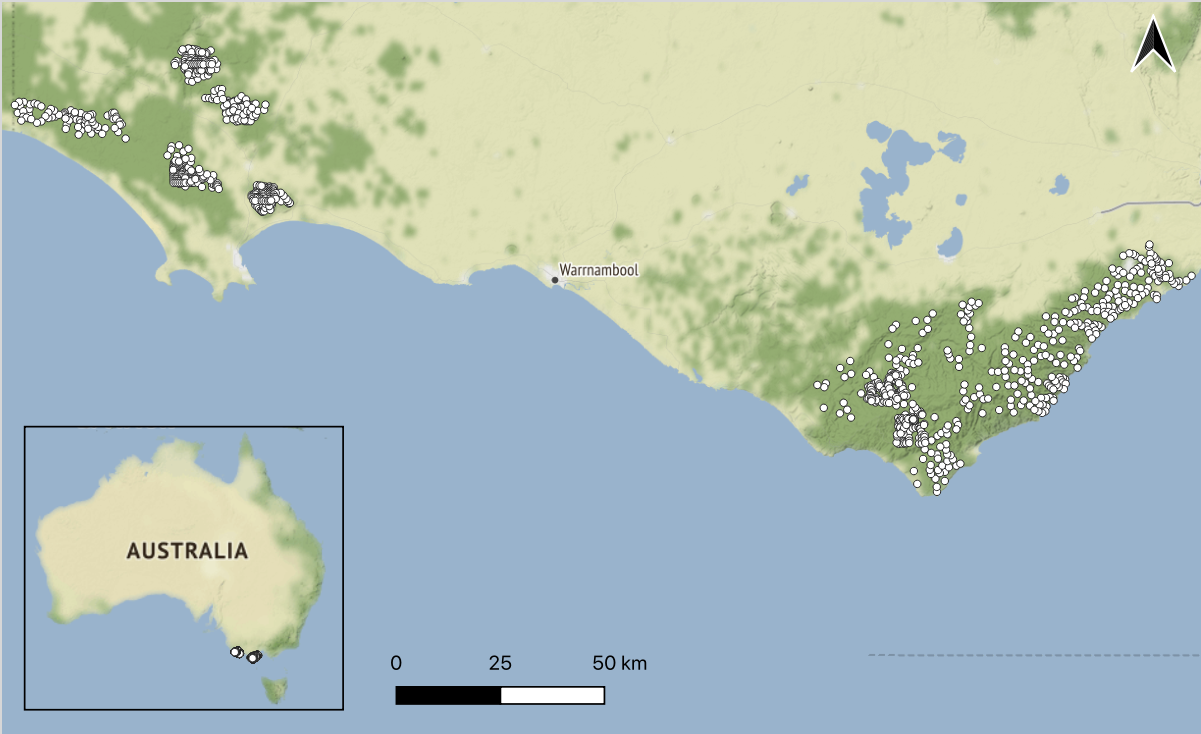
\includegraphics[width=1\linewidth]{../figs/map_cams} 

}

\caption{Locations of our study regions in south-west Victoria, Australia. The grids of camera-traps are denoted by white dots. The Glenelg region is to the west and Otway region to the east. Native vegetation is indicated by dark green, with hill shading. \textit{Map tiles by Stamen Design, under CC BY 3.0, map data by OpenStreetMap, under CC BY SA.}}\label{fig:diel-map}
\end{figure}

\newpage

\hypertarget{results}{%
\section{RESULTS}\label{results}}

Overall, we collated 5449 and 2202 independent detections of foxes and cats, respectively (separated by at least 30 minutes) from 172,052 camera-trap nights (Table \ref{tab:diel-tab1}).

\hypertarget{how-does-predator-overall-activity-and-diel-activity-patterns-vary-across-space-model-1-1}{%
\subsubsection{How does predator overall activity and diel activity patterns vary across space? (model 1)}\label{how-does-predator-overall-activity-and-diel-activity-patterns-vary-across-space-model-1-1}}

Predator activity varied considerably across space and throughout the 24-hour daily cycle, and there was some variation in the predator diel activity patterns across space. On average, both predators showed similar diel activity patterns: mostly nocturnal with peaks in activity around sunrise and sunset (i.e., crepuscular; Fig. \ref{fig:diel-veg}i). The main difference between the species was that fox activity peaked just after sunset and they were less likely to be active during the day than cats. Cats also tended to be more active at sunset relative to sunrise.

Diel activity pattern strength also differed between the species. Fox activity was concentrated strongly at particular times of the day, especially in the Glenelg region where activity varied by up to 371\% throughout the daily cycle (Fig. \ref{fig:diel-space}a). Feral cats had relatively more consistent activity throughout the daily cycle and across regions; the maximum difference in cat activity throughout the daily cycle for any given location was 185\%.

Variation in diel activity patterns across space, as well as differences in overall activity between the predators, was strongest in the Otway Ranges. For example, overall fox activity (Fig. \ref{fig:diel-space-o-fox}) and diel activity pattern strength (Fig. \ref{fig:diel-space}b) were lowest in the south-west Otway Ranges, while feral cat overall activity (Fig. \ref{fig:diel-space-o-cat}) and diel activity pattern strength (Fig. \ref{fig:diel-space}b) were highest in that subregion.

\hypertarget{how-does-predator-overall-activity-and-diel-activity-patterns-vary-across-vegetation-types-model-2-1}{%
\subsubsection{How does predator overall activity and diel activity patterns vary across vegetation types? (model 2)}\label{how-does-predator-overall-activity-and-diel-activity-patterns-vary-across-vegetation-types-model-2-1}}

Overall levels of fox activity were similar across all vegetation types, except wet forests where fox activity was considerably lower. Overall cat activity was more variable across vegetation types; lowest in heathy woodlands and highest in wet forests (Fig. \ref{fig:diel-veg}b).

Diel activity patterns for foxes were similar across all vegetation type except wet forests; in wet forests, foxes were consistently active throughout the daily cycle (Fig. \ref{fig:diel-veg}a). On the other hand, cats were nocturnal (and most active) in wet forests, but largely crepuscular in all other vegetation types (Fig. \ref{fig:diel-veg}b). For both predators, the random effect for region (Glenelg or Otways) in the vegetation models shrank to near-zero, indicating all variation between the regions was explained by the vegetation covariate and site random intercept.

\hypertarget{do-feral-cats-avoid-foxes-in-space-or-time-model-3-1}{%
\subsubsection{Do feral cats avoid foxes in space or time? (model 3)}\label{do-feral-cats-avoid-foxes-in-space-or-time-model-3-1}}

Cat spatial activity was relatively unaffected by the fox activity in both habitat types of the Otway Ranges; and, if anything, increased with increasing adjusted fox counts in the Glenelg region (Fig. \ref{fig:diel-cat-fox}), indicating cats did not avoid foxes spatially.

Across all habitat types, feral cat diel activity patterns changed across the gradient of fox activity (Fig. \ref{fig:diel-cat-fox}). In the Glenelg region and Otway dry habitat types, feral cats had a nocturnal-crepuscular diel activity pattern where fox activity was low, but were most active during the day where fox activity was high. In contrast, in the wet forests of the Otway Ranges, feral cats were more strongly nocturnal when fox activity was high.

\newpage

\begin{figure}

{\centering 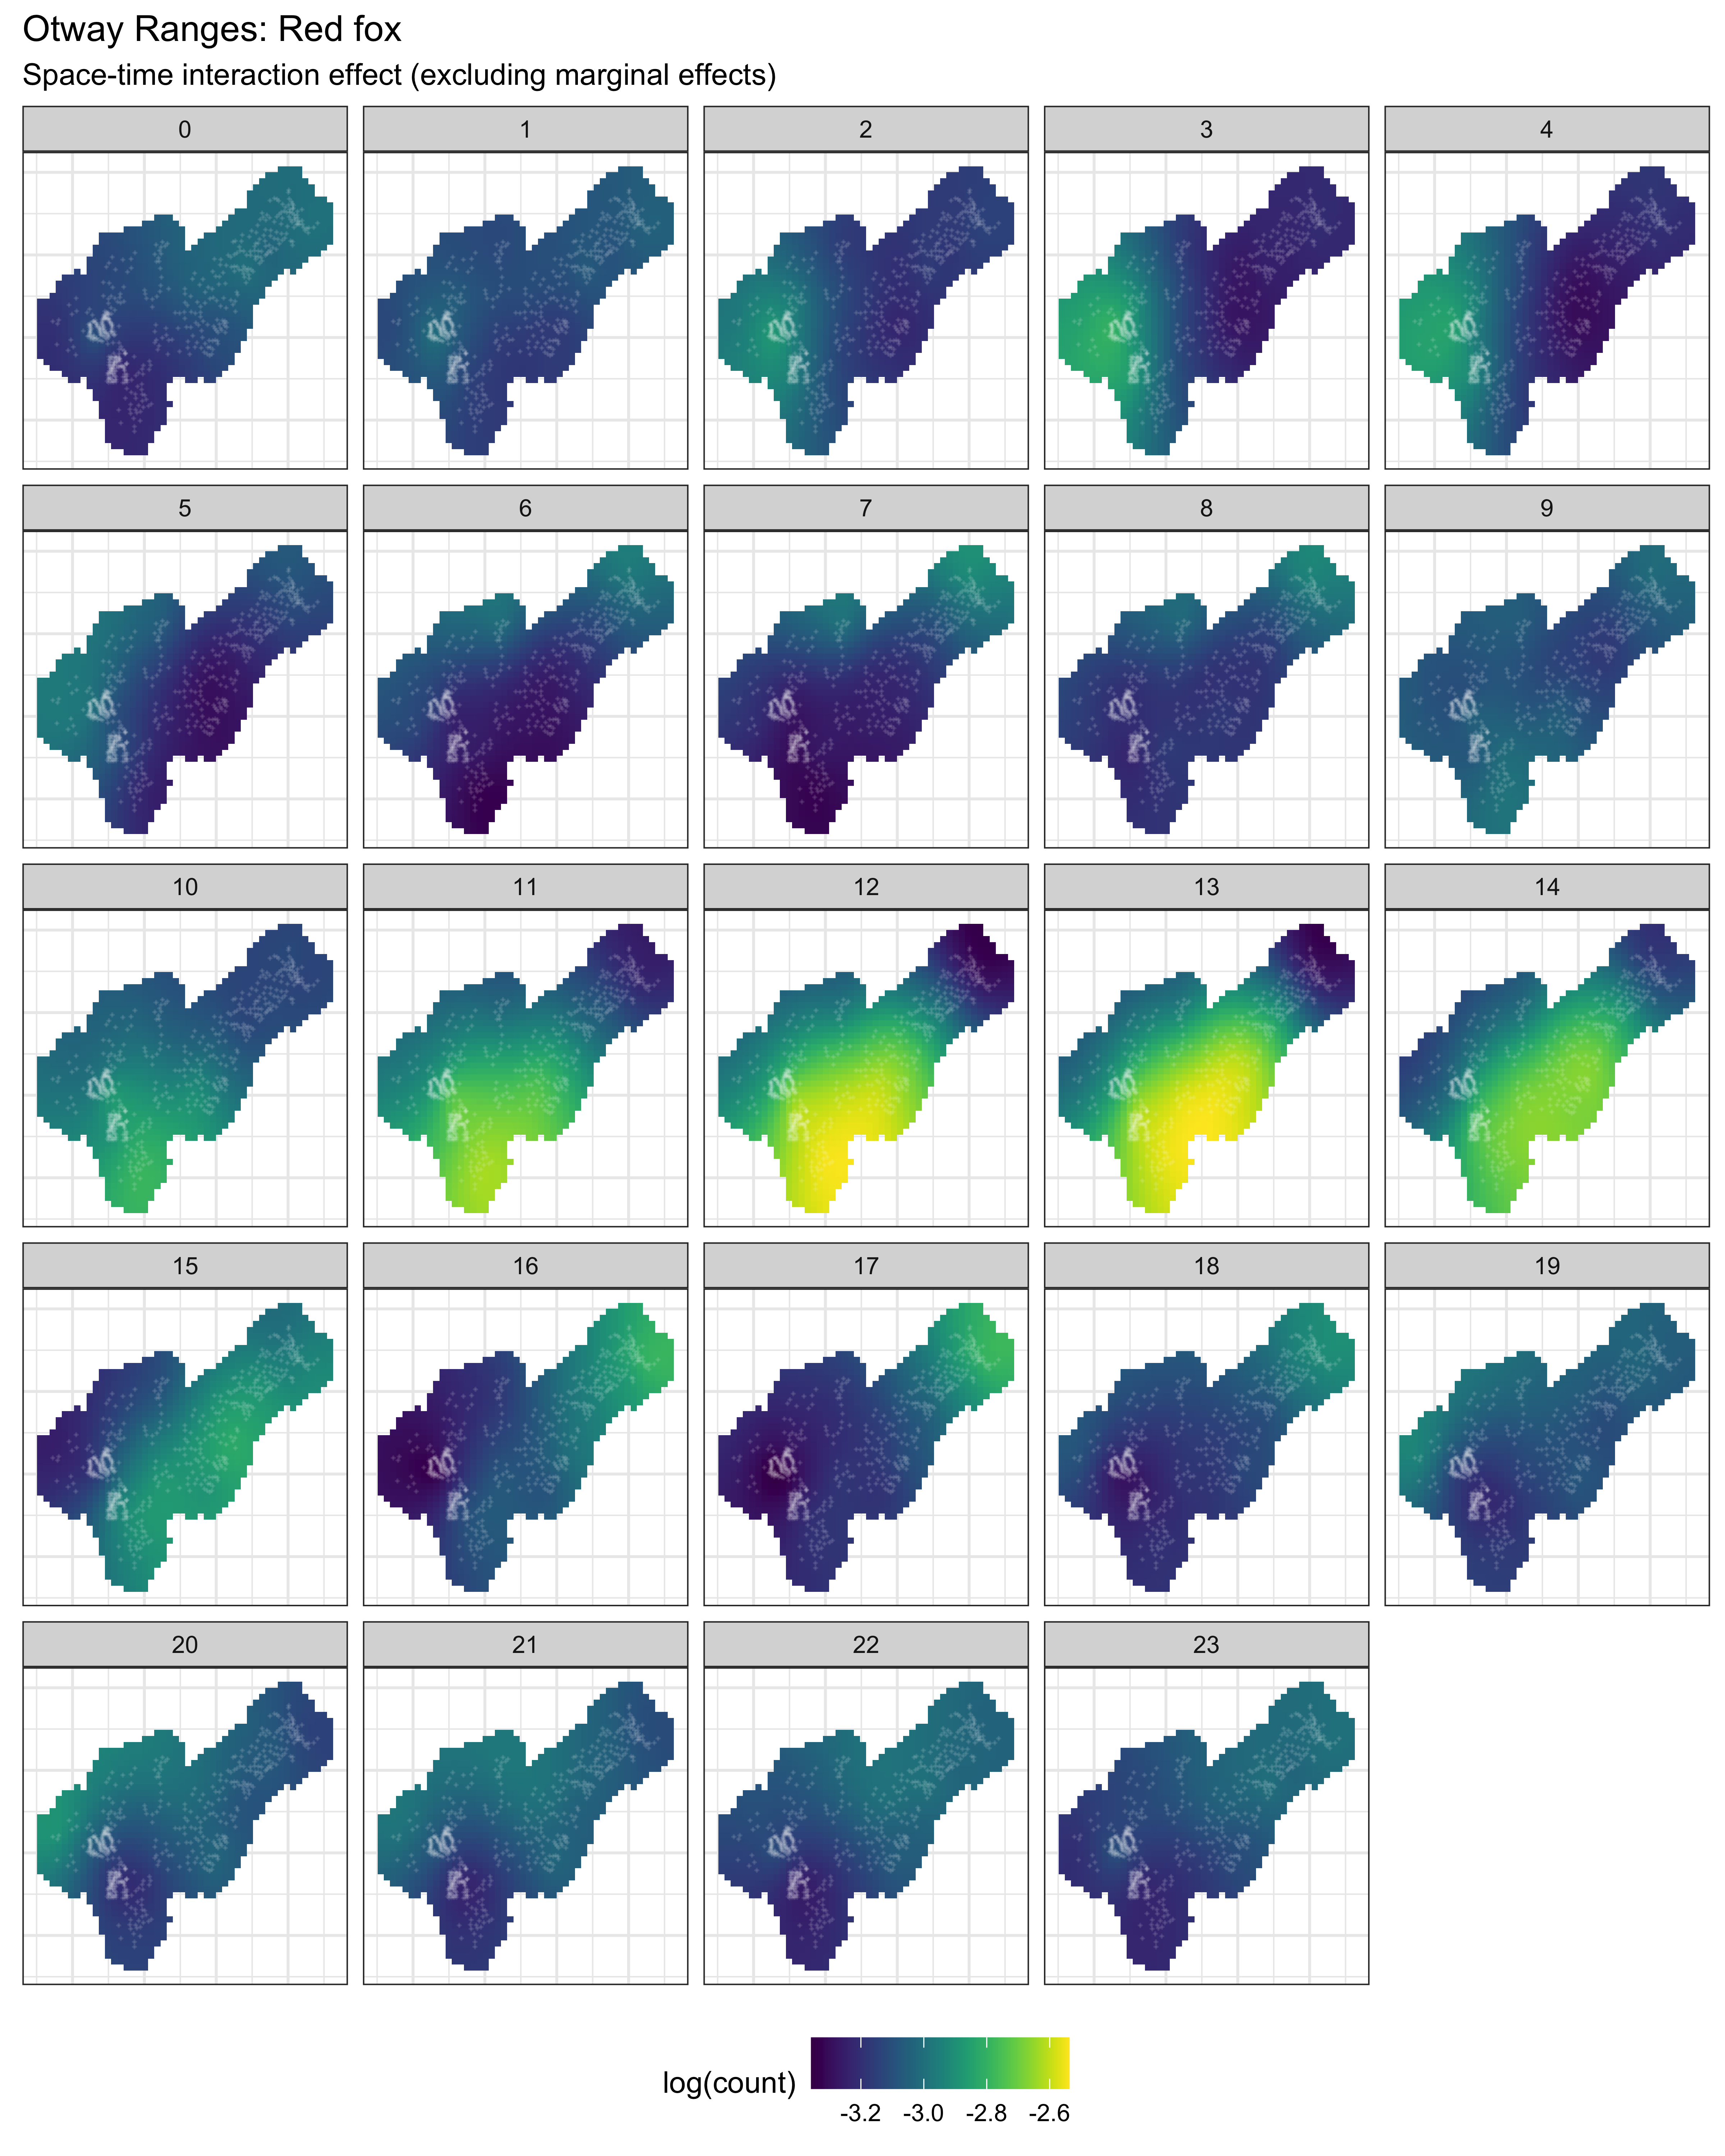
\includegraphics[width=1\linewidth]{../figs/spte_diff_avg_o_fox} 

}

\caption{Interaction effect of space-time on red fox \textit{Vulpes vulpes} activity across each hour of the day (0 - 23) in the Otway Ranges, Australia (model 1), as an example. Corresponding plots for feral cats \textit{Felis catus} in this region, as well as both predators in the Glenelg region are provided in the Supporting Information, as are the marginal effects of space and time. White crosses depict unique camera-trap sites.}\label{fig:diel-st-int-o-fox}
\end{figure}

\begin{figure}

{\centering 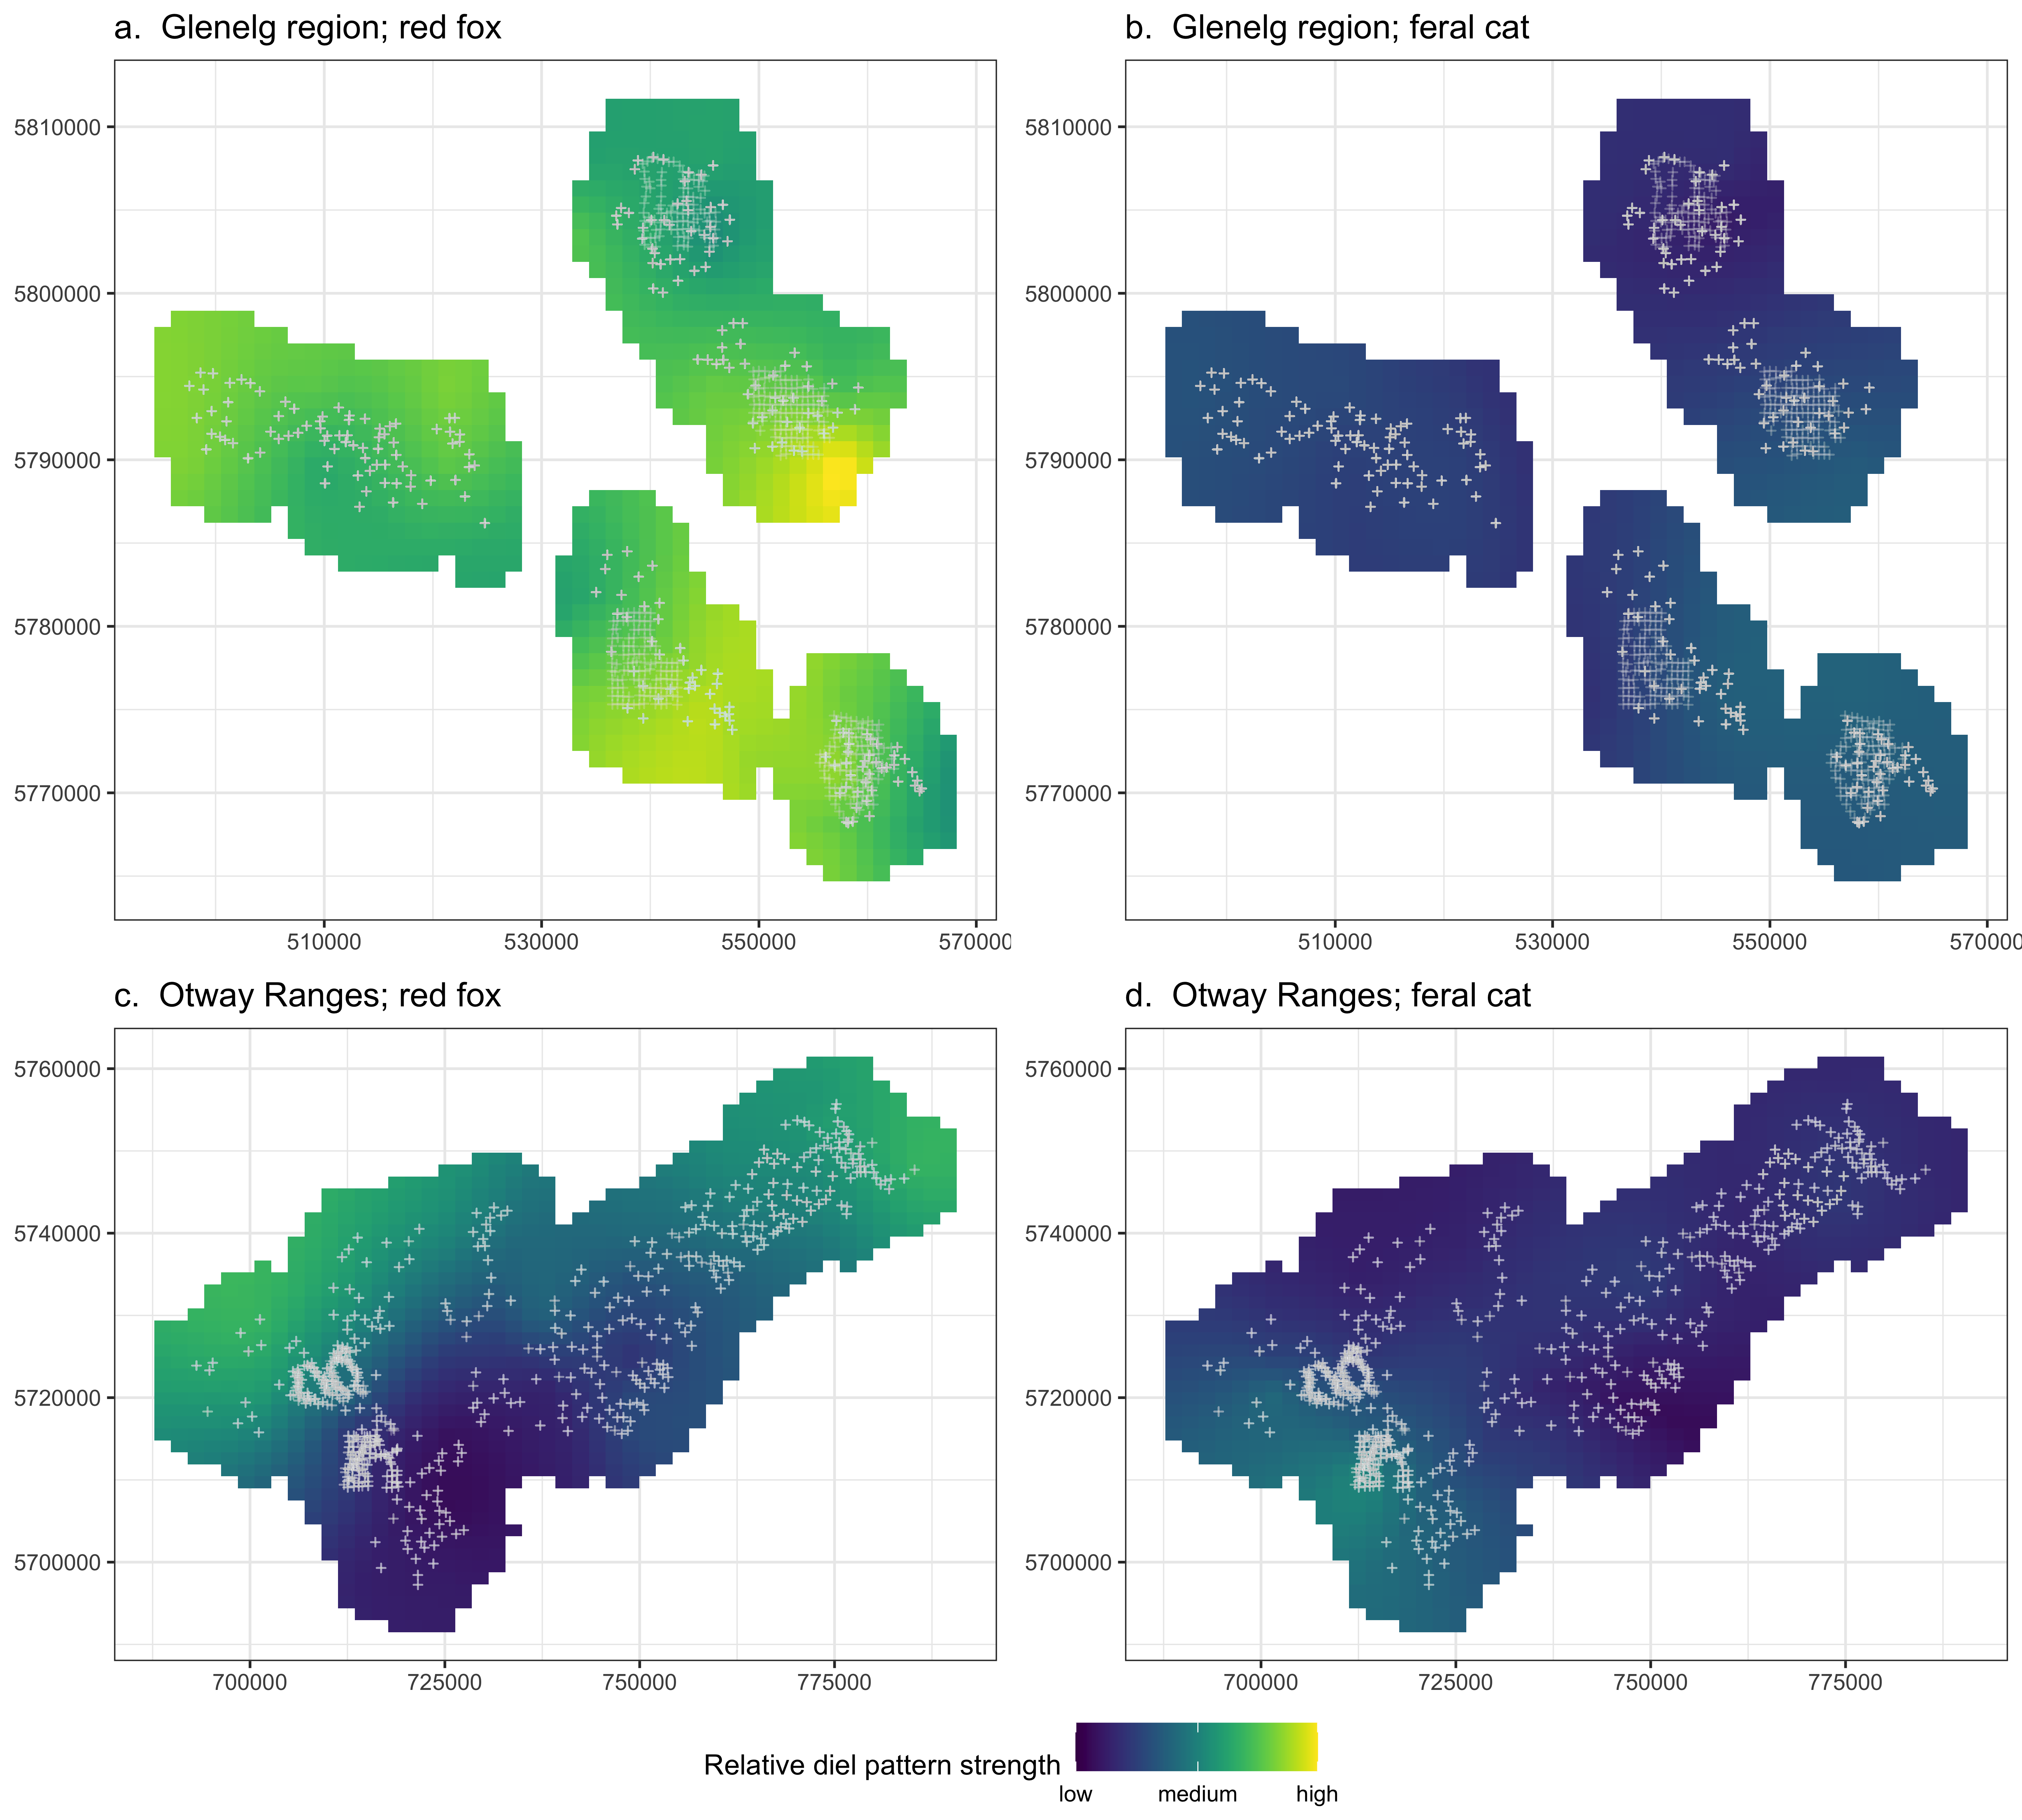
\includegraphics[width=1\linewidth]{../figs/diel_strength_600dpi} 

}

\caption{The strength of diel activity patterns of two invasive predators varied within the two study regions in south-west Victoria, Australia (model 1). White crosses depict unique camera-trap sites; colour brightness scales with increasing percentage difference between the minimum and maximum activity estimate over the 24-hour cycle for each location. Red foxes \textit{Vulpes vulpes} (a, c) concentrated their activity during particular times of the day, especially in the Glenelg region (a) and the drier parts of the Otways (c), whereas feral cat \textit{Felis catus} activity was relatively consistent activity throughout the daily cycle (b, d).}\label{fig:diel-space}
\end{figure}

\newpage

\begin{figure}

{\centering 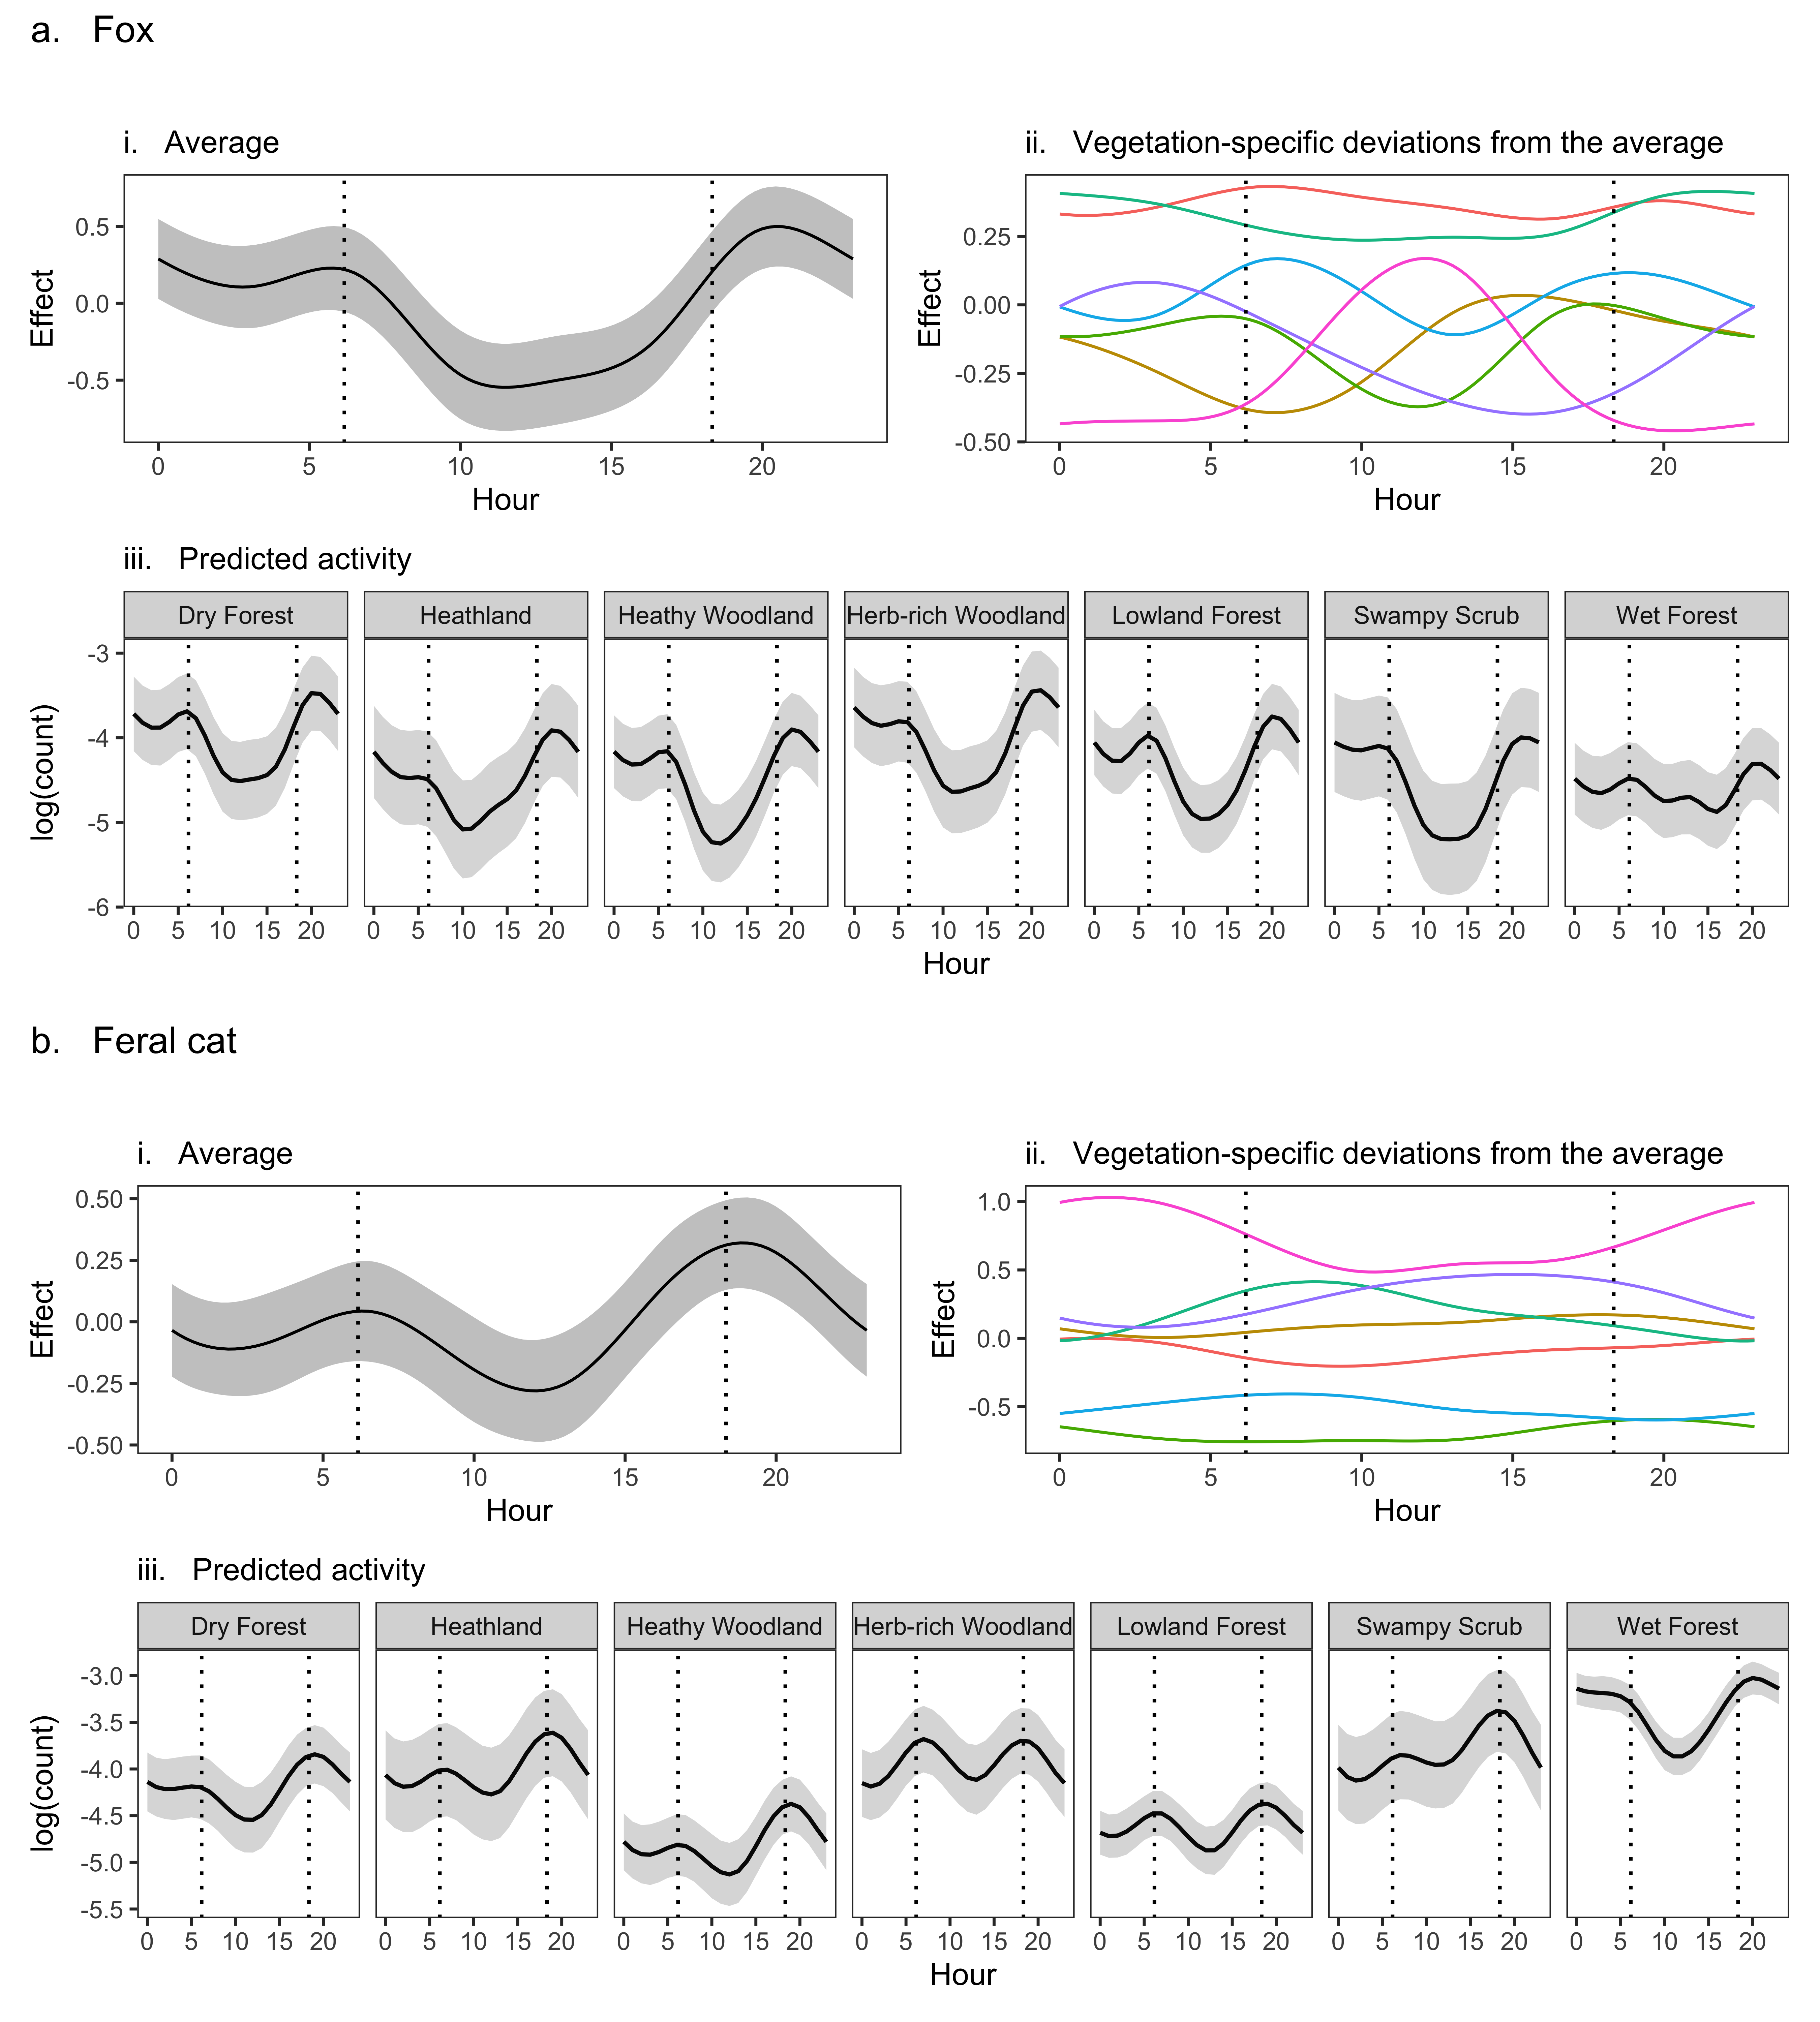
\includegraphics[width=1\linewidth]{../figs/predator_veg} 

}

\caption{Red foxes \textit{Vulpes vulpes} (a) and feral cat \textit{Felis catus} (B) diel activity patterns overall (i) and across different Ecological Vegetation Class (EVC) groups (ii, iii) in south-west Victoria, Australia (model 2). Dotted, vertical lines represent average sunrise and sunset times. Shaded areas indicate 95\% confidence intervals. Both invasive predators had a crepuscular to nocturnal diel activity pattern on average, with slight deviations across the drier EVC groups and large deviations in wet forests (ii; wet forests shown as pink line). The overall level of activity was relatively consistent across EVC groups for foxes (a – iii), whereas it differed substantially for feral cats (b - iii).}\label{fig:diel-veg}
\end{figure}

\newpage

\begin{figure}

{\centering 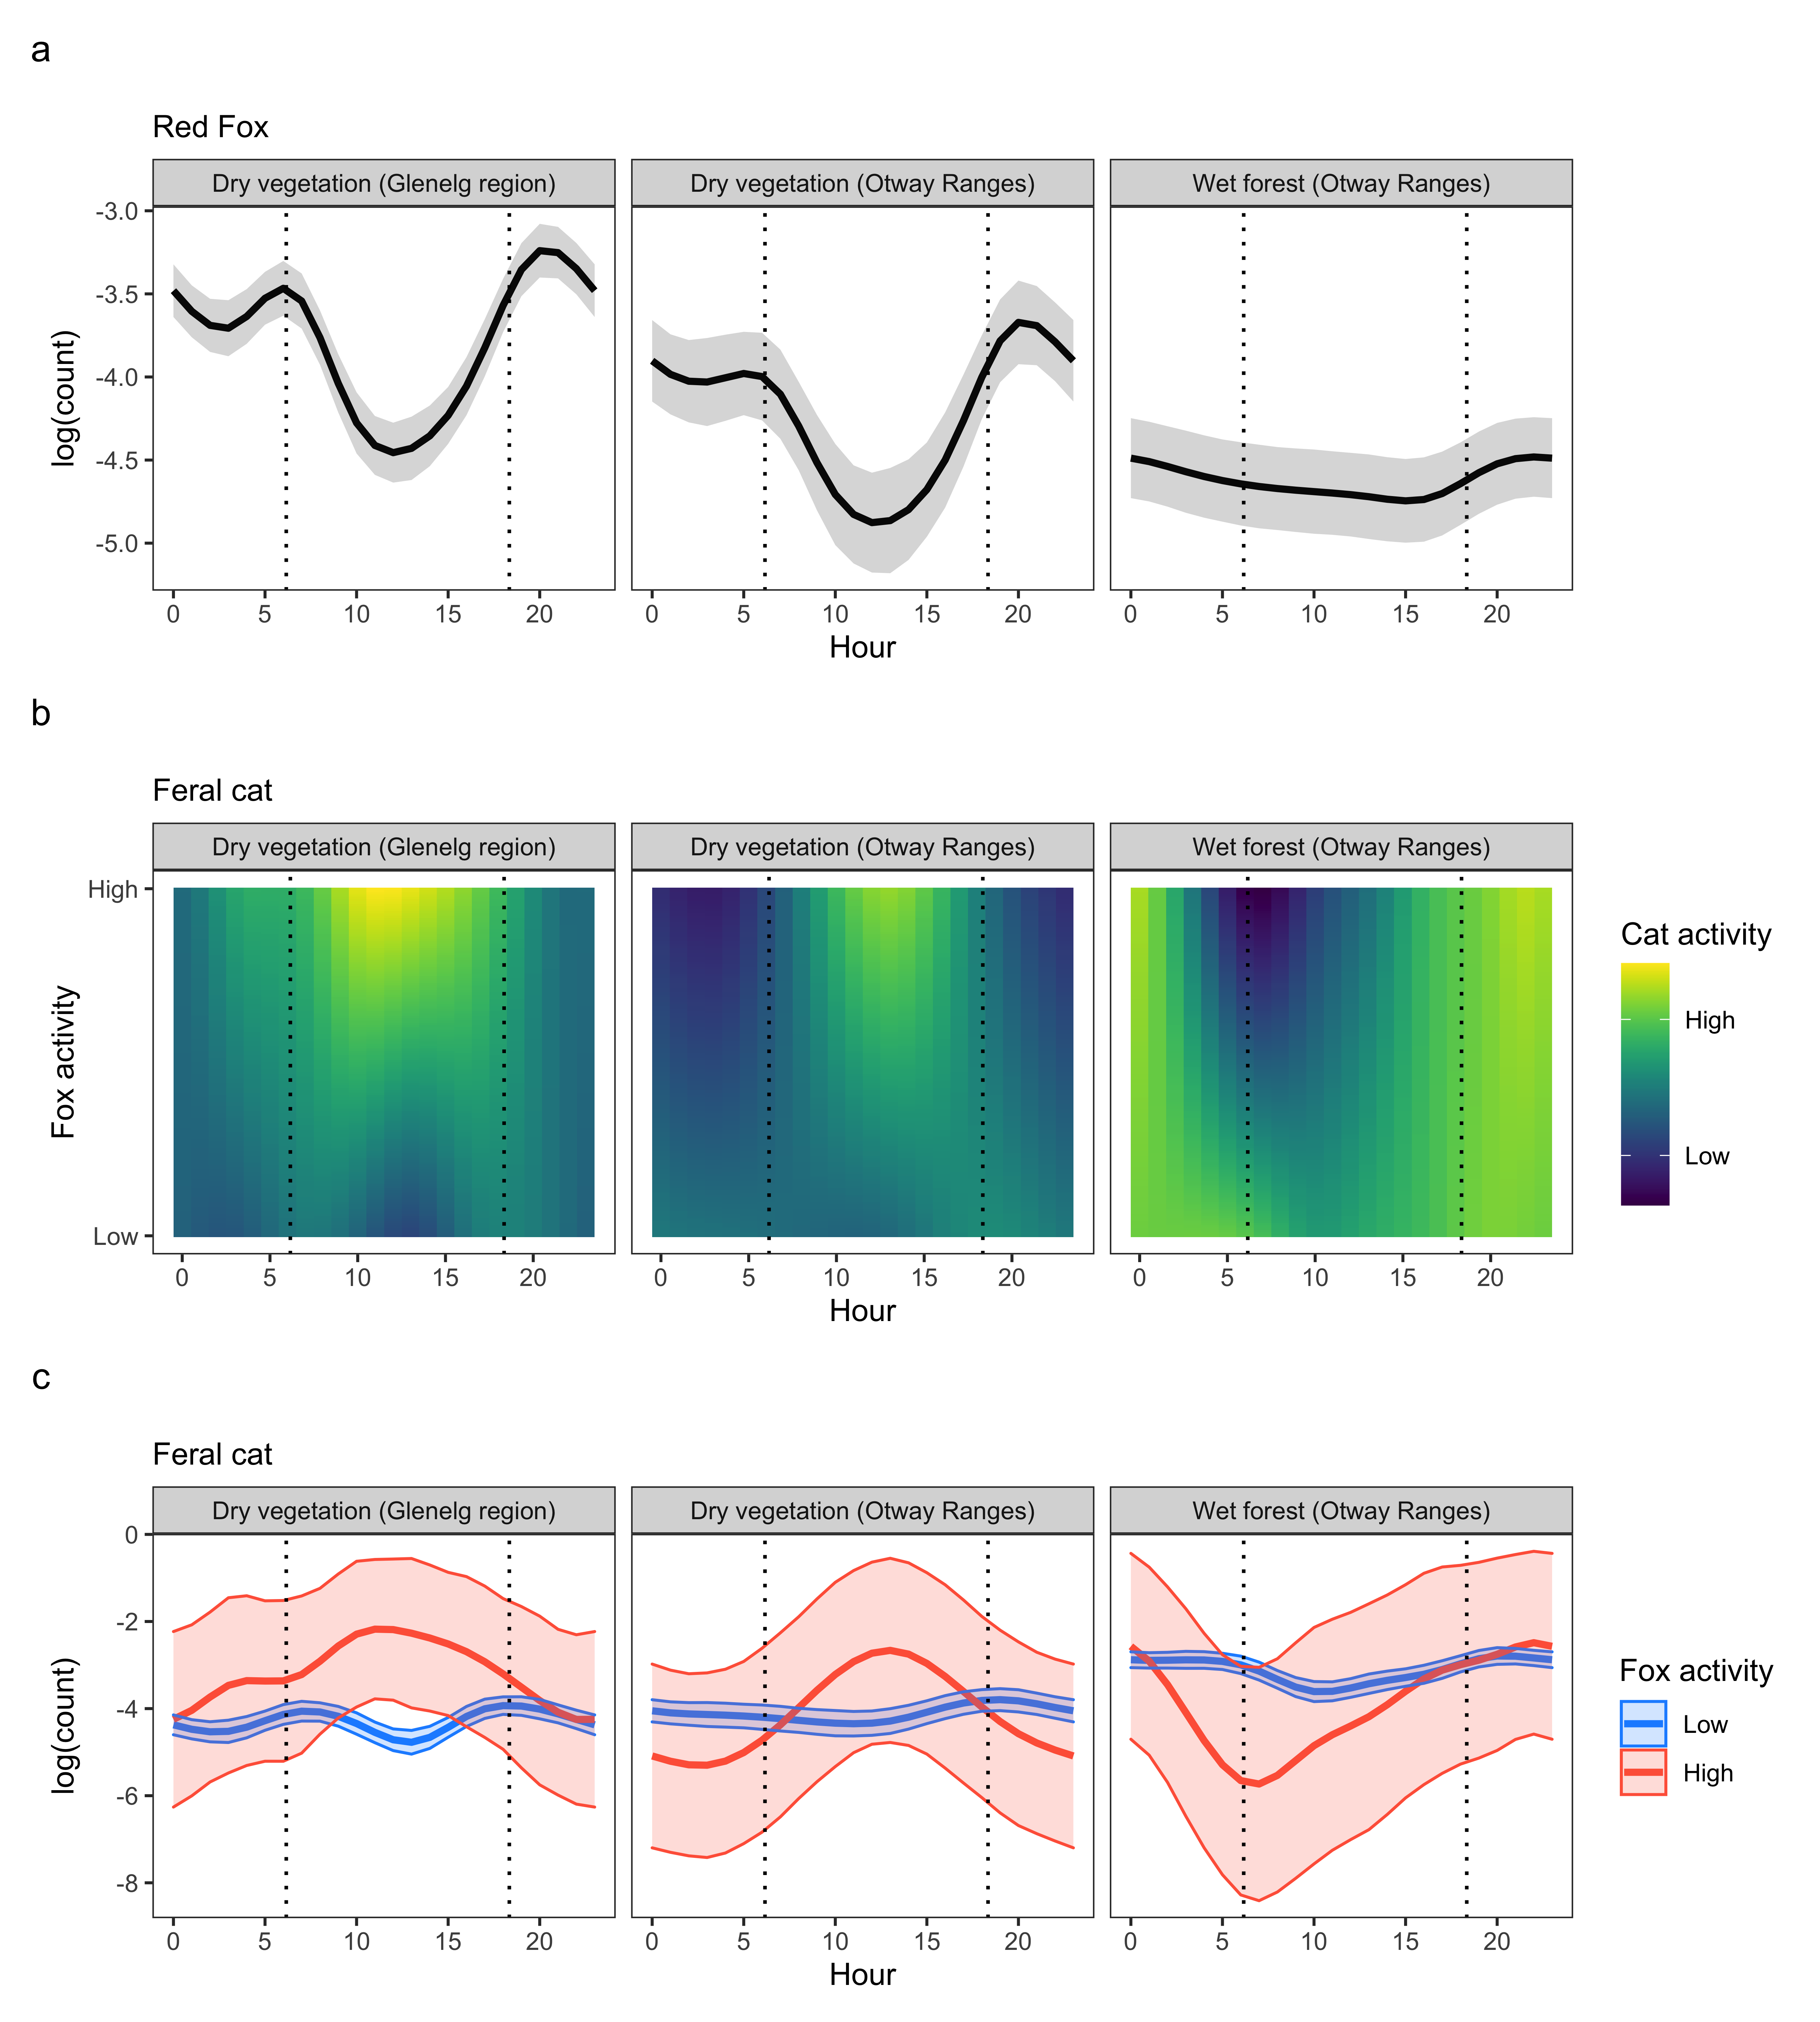
\includegraphics[width=1\linewidth]{../figs/cat_fox_count} 

}

\caption{Variation in mean feral cat \textit{Felis catus} activity (a) and associated uncertainty estimates (b) in response to count of ’independent’ red fox \textit{Vulpes vulpes} detections (log-transformed and survey effort adjusted) across each ’habitat type’ in south-west Victoria, Australia (model 3). Grey vertical lines represent average sunrise and sunset times. In the Glenelg region, there were more feral cat detections where there were more fox detections, but cat peak diel activity shifted from crepuscular night to pre-dawn and midday (a). In the Otway Ranges, feral cat activity also peaked during the day where fox activity was high in dry vegetation types (b), but was more nocturnal where fox activity was high in the rainforests and wet forests (c).}\label{fig:diel-cat-fox}
\end{figure}

\newpage

\hypertarget{discussion}{%
\section{DISCUSSION}\label{discussion}}

A key question in ecological theory is whether animals are evolutionary hardwired to occupy particular temporal niches, or have circadian rhythms that are responsive to changing environmental conditions and interactions with other species (Schoener 1974; Daan 1981; Lima \& Dill 1990). Here we demonstrate that diel activity patterns are not fixed, but vary across space based on landscape context and fear. In our study, sympatric invasive predators had similar diel activity patterns when averaged across broad regions (i.e., high circular overlap; Fig. \ref{fig:diel-space-time-marginal}; as did Roshier \& Carter 2021), but behaviours varied considerably within landscapes. Fox daily activity patterns were most strongly tied to the daily cycle in dry habitat types, but showed little diel activity pattern in the wet forests (Fig. \ref{fig:diel-veg}a). In contrast, cats were mostly nocturnal in wet forests but crepuscular in dry vegetation types (Fig. \ref{fig:diel-veg}b). Within broad habitat types, cats altered their diel activity patterns at sites with higher fox activity (Fig. \ref{fig:diel-cat-fox}). Control programs that reduce invasive fox activity are therefore likely to change cat diel activity patterns, which in turn may alter cat impacts on native prey species. Quantifying changes in diel activity patterns provides important context for understanding species interactions, which is key for effective ecosystem management (Gaynor \emph{et al.} 2021).

Shifting diel activity patterns may facilitate spatial coexistence of dominant and subordinate species (Carothers \& Jaksić 1984). For cats, altering diel activity patterns to less-preferred times of day may be worthwhile to persist in high-quality habitat. Few studies have demonstrated predator-induced shifts in diel activity (Kronfeld-Schor \& Dayan 2003), but notably, ship rats \emph{Rattus norvegicus} were also found to switch from nocturnal to diurnal behaviour in response to fox activity (Fenn \& Macdonald 1995) and a similar nocturnal-diurnal shift was observed in American mink \emph{Neovison vison} following the recolonisation of native predators (Harrington \emph{et al.} 2009). For cats in our study, a switch to diurnal behaviour where fox activity was high in the dry vegetation types may have been facilitated by the higher abundance of reptiles in these habitat types relative to wet forests (which are mostly diurnal; Woinarski \emph{et al.} 2018). At wet forest sites with high fox activity, cats concentrated their activity away from sunrise and sunset towards midnight, despite a diurnal shift appearing to similarly reduce the risk of a fox encounter. In this situation, we expect becoming more nocturnal to be favourable over a diurnal shift because this is when small mammals are active and cats would be least visible to foxes (cats here mostly had black or grey coats). Overall fox activity was twice as low in the wet forests relative to dry habitat types, and so cats were likely under less pressure to radically alter their diel activity patterns. Understanding how these potential avoidance behaviours impacts native prey is a key research priority to improve invasive predator management.

Cats may have avoided foxes in time, but we saw no sign of spatial avoidance (i.e.~no fine-scale negative association between fox and cat overall activity (Fig. \ref{fig:diel-cat-fox}b:c). Overlap in spatial activity at fine scales (i.e., at the level of camera-trap sites) may have been facilitated by temporal avoidance (Kronfeld-Schor \& Dayan 2003). However, we considered spatial avoidance across the entire survey duration (averaging 47 days). Cats may indeed avoid foxes spatially, but transiently on the scale of hours to days---after all, how is a cat to know where to avoid a fox without encountering signs of one? Short-term spatial avoidance is quite plausible given foxes mark territories using scats and odours, which cats could tangibly associate with high risk shortly after. Temporary spatial avoidance could be tested using decay curves (e.g., Niedballa \emph{et al.} 2019). Alternatively, no sign of spatial avoidance between these invasive predators could also be an artefact of the quality of camera set-up and hence detectability. The 3667 camera-traps were deployed by numerous people, and the quality of set-ups differed considerably in terms of detecting predators. Camera-traps that angled only slightly downwards, rather than upwards or strongly downwards, seemed most effective at detecting both predator species (M.W Rees, personal observation). Predator interactions are routinely inferred through spatial associations between species; however such analyses are subject to numerous pitfalls which can make inference unreliable (reviewed in Blanchet, Cazelles, \& Gravel 2020).\\
A distinction of our study from others is that we modelled potential avoidance behaviours in a simple predator guild, where apex predator activity was artificially manipulated. This reduces potential bias from differences in niche preferences and the unmodelled impacts of other predators in the system. We also included replication across different habitat types. However, because our study did not consider associations with prey species, we cannot distinguish whether changes in cat diel activity patterns were the result of direct fox avoidance or indirect associations with shared prey. For example, low fox activity may promote the availability of a preferred shared prey species with a diel pattern which differs from those of cats on average, and as a result, cats might shift diel activity patterns at sites with low fox activity to more closely match those of the more abundant prey species. We would expect introduced European rabbits \emph{Oryctolagus cuniculus} and hares \emph{Lepus europaeus} (which are diurnal) to be particularly likely to induce such a response in dry vegetation types (McGregor \emph{et al.} 2020; Stobo-Wilson \emph{et al.} 2020), however, rabbits and hares are rare within the natural vegetation of the landscapes we surveyed (only ever being detected at 40 of 1232 sites) and there is little evidence that predation by foxes suppresses rabbit populations (Norbury \& Jones 2015; Scroggie \emph{et al.} 2018). While of particular interest, whether temporal fox-cat interactions are direct or indirect does not change the resulting impact on native prey, and hence the outcomes of fox management.

Flexible antipredator behaviours make evolutionary sense, but have been rarely demonstrated in terms of spatiotemporal predator avoidance (although, see Relyea 2003; Brown \emph{et al.} 2013; Cunningham \emph{et al.} 2019), because this often requires manipulative experiments or at least more complicated models (Kronfeld-Schor \& Dayan 2003). Our study demonstrates that GAMs offer a powerful tool for modelling continuous shifts in animal activity across both space and time, capable of capturing complex interactions and sharing information across categorical variables. The inbuilt smoothing penalties are another benefit of GAMs over kernel density estimation (Ridout \& Linkie 2009), in which noisy data can produce spurious estimates (Frey \emph{et al.} 2017; Iannarilli \emph{et al.} 2019). The alternative approach of simply comparing average diel activity overlap between two species (Ridout \& Linkie 2009) would have been misleading for two reasons. Firstly, predator diel activity patterns varied `naturally' across heterogeneous landscapes (requiring avoidance to be tested in wet forests and dry vegetation types separately; Fig. \ref{fig:diel-veg}). Secondly, apex predator temporal avoidance strategies were not consistently employed, but depended on overall apex predator activity and vegetation type (Fig. \ref{fig:diel-cat-fox}). Despite their underlying statistical complexity, GAMs in the `mgcv' R-package are straightforward to fit. Our GAM framework for modelling spatiotemporal activity can be used on any species with time-stamped detections, including datasets with categorical or continuous covariates and hierarchical groupings.

Animal diel activity patterns can be complex, varying across space, habitat types and threat-levels. Despite telling an important story about how animals interact with each other and the environment, detection times are commonly discarded from statistical analyses of camera-trap data. In the rare instances that they are considered, diel activity patterns are predominantly estimated at the population-level, overlooking finer-scale behaviours that can affect fitness, survival and ecosystem-impacts. Our results demonstrate the importance of (a) considering diel activity in regards to species interactions, (b) modelling changes in animal behaviour rather than overlap with other species, and (c) testing avoidance behaviours within a joint spatiotemporal framework. Our study adds to the limited body of evidence that top predators can produce a landscape of fear which is powerful enough to reverse the diel activity patterns of subordinate species (Kronfeld-Schor \& Dayan 2003).

\newpage

\hypertarget{acknowledgements}{%
\section*{ACKNOWLEDGEMENTS}\label{acknowledgements}}
\addcontentsline{toc}{section}{ACKNOWLEDGEMENTS}

\newpage

\hypertarget{references}{%
\section*{REFERENCES}\label{references}}
\addcontentsline{toc}{section}{REFERENCES}

\hypertarget{refs}{}
\leavevmode\hypertarget{ref-anderson2001need}{}%
Anderson, D.R. (2001) The need to get the basics right in wildlife field studies. \emph{Wildlife Society Bulletin}, 1294--1297.

\leavevmode\hypertarget{ref-basille2015plastic}{}%
Basille, M., Fortin, D., Dussault, C., Bastille-Rousseau, G., Ouellet, J.-P. \& Courtois, R. (2015) Plastic response of fearful prey to the spatiotemporal dynamics of predator distribution. \emph{Ecology}, \textbf{96}, 2622--2631.

\leavevmode\hypertarget{ref-maptools}{}%
Bivand, R. \& Lewin-Koh, N. (2021) \emph{Maptools: Tools for Handling Spatial Objects}.

\leavevmode\hypertarget{ref-guillaume2020co}{}%
Blanchet, F.G., Cazelles, K. \& Gravel, D. (2020) Co-occurrence is not evidence of ecological interactions. \emph{Ecology Letters}, \textbf{23}, 1050--1063.

\leavevmode\hypertarget{ref-brashares2010ecological}{}%
Brashares, J.S., Prugh, L.R., Stoner, C.J. \& Epps, C.W. (2010) Ecological and conservation implications of mesopredator release. \emph{Trophic cascades: Predators, prey, and the changing dynamics of nature} pp. 221--240. Island Press.

\leavevmode\hypertarget{ref-brown2013phenotypically}{}%
Brown, G.E., Ferrari, M.C., Elvidge, C.K., Ramnarine, I. \& Chivers, D.P. (2013) Phenotypically plastic neophobia: A response to variable predation risk. \emph{Proceedings of the Royal Society B: Biological Sciences}, \textbf{280}, 20122712.

\leavevmode\hypertarget{ref-brown1999ecology}{}%
Brown, J.S., Laundré, J.W. \& Gurung, M. (1999) The ecology of fear: Optimal foraging, game theory, and trophic interactions. \emph{Journal of Mammalogy}, \textbf{80}, 385--399.

\leavevmode\hypertarget{ref-carothers1984time}{}%
Carothers, J.H. \& Jaksić, F.M. (1984) Time as a niche difference: The role of interference competition. \emph{Oikos}, 403--406.

\leavevmode\hypertarget{ref-comer2020integrating}{}%
Comer, S., Clausen, L., Cowen, S., Pinder, J., Thomas, A., Burbidge, A.H., Tiller, C., Algar, D. \& Speldewinde, P. (2020) Integrating feral cat \emph{(Felis catus)} control into landscape-scale introduced predator management to improve conservation prospects for threatened fauna: A case study from the south coast of Western Australia. \emph{Wildlife Research}, \textbf{47}, 762--778.

\leavevmode\hypertarget{ref-creel2008relationships}{}%
Creel, S. \& Christianson, D. (2008) Relationships between direct predation and risk effects. \emph{Trends in Ecology \& Evolution}, \textbf{23}, 194--201.

\leavevmode\hypertarget{ref-cunningham2019temporal}{}%
Cunningham, C.X., Scoleri, V., Johnson, C.N., Barmuta, L.A. \& Jones, M.E. (2019) Temporal partitioning of activity: Rising and falling top-predator abundance triggers community-wide shifts in diel activity. \emph{Ecography}, \textbf{42}, 2157--2168.

\leavevmode\hypertarget{ref-daan1981adaptive}{}%
Daan, S. (1981) Adaptive daily strategies in behavior. \emph{Biological rhythms} pp. 275--298. Springer Publishing.

\leavevmode\hypertarget{ref-delwp2020bioregions}{}%
Department of Environment, Land, Water \& Planning. (2020) Bioregions and EVC Benchmarks, \url{https://www.environment.vic.gov.au/biodiversity/bioregions-and-evc-benchmarks}

\leavevmode\hypertarget{ref-doherty2016invasive}{}%
Doherty, T.S., Glen, A.S., Nimmo, D.G., Ritchie, E.G. \& Dickman, C.R. (2016) Invasive predators and global biodiversity loss. \emph{Proceedings of the National Academy of Sciences}, \textbf{113}, 11261--11265.

\leavevmode\hypertarget{ref-doherty2017stop}{}%
Doherty, T.S. \& Ritchie, E.G. (2017) Stop jumping the gun: A call for evidence-based invasive predator management. \emph{Conservation Letters}, \textbf{10}, 15--22.

\leavevmode\hypertarget{ref-estes2011trophic}{}%
Estes, J.A., Terborgh, J., Brashares, J.S., Power, M.E., Berger, J., Bond, W.J., Carpenter, S.R., Essington, T.E., Holt, R.D., Jackson, J.B. \& others. (2011) Trophic downgrading of planet earth. \emph{Science}, \textbf{333}, 301--306.

\leavevmode\hypertarget{ref-fenn1995use}{}%
Fenn, M.G. \& Macdonald, D.W. (1995) Use of middens by red foxes: Risk reverses rhythms of rats. \emph{Journal of Mammalogy}, \textbf{76}, 130--136.

\leavevmode\hypertarget{ref-frey2017investigating}{}%
Frey, S., Fisher, J.T., Burton, A.C. \& Volpe, J.P. (2017) Investigating animal activity patterns and temporal niche partitioning using camera-trap data: Challenges and opportunities. \emph{Remote Sensing in Ecology and Conservation}, \textbf{3}, 123--132.

\leavevmode\hypertarget{ref-gaynor2019landscapes}{}%
Gaynor, K.M., Brown, J.S., Middleton, A.D., Power, M.E. \& Brashares, J.S. (2019) Landscapes of fear: Spatial patterns of risk perception and response. \emph{Trends in Ecology \& Evolution}, \textbf{34}, 355--368.

\leavevmode\hypertarget{ref-gaynor2021applied}{}%
Gaynor, K.M., Cherry, M.J., Gilbert, S.L., Kohl, M.T., Larson, C.L., Newsome, T.M., Prugh, L.R., Suraci, J.P., Young, J.K. \& Smith, J.A. (2021) An applied ecology of fear framework: Linking theory to conservation practice. \emph{Animal Conservation}, \textbf{24}, 308--321.

\leavevmode\hypertarget{ref-glen2005complex}{}%
Glen, A.S. \& Dickman, C.R. (2005) Complex interactions among mammalian carnivores in Australia, and their implications for wildlife management. \emph{Biological Reviews}, \textbf{80}, 387--401.

\leavevmode\hypertarget{ref-harrington2009impact}{}%
Harrington, L.A., Harrington, A.L., Yamaguchi, N., Thom, M.D., Ferreras, P., Windham, T.R. \& Macdonald, D.W. (2009) The impact of native competitors on an alien invasive: Temporal niche shifts to avoid interspecific aggression. \emph{Ecology}, \textbf{90}, 1207--1216.

\leavevmode\hypertarget{ref-DHARMa}{}%
Hartig, F. (2020) \emph{DHARMa: Residual Diagnostics for Hierarchical (Multi-Level / Mixed) Regression Models}.

\leavevmode\hypertarget{ref-hradsky2017bayesian}{}%
Hradsky, B.A., Penman, T.D., Ababei, D., Hanea, A., Ritchie, E.G., York, A. \& Di Stefano, J. (2017) Bayesian networks elucidate interactions between fire and other drivers of terrestrial fauna distributions. \emph{Ecosphere}, \textbf{8}, e01926.

\leavevmode\hypertarget{ref-hunter2018not}{}%
Hunter, D.O., Lagisz, M., Leo, V., Nakagawa, S. \& Letnic, M. (2018) Not all predators are equal: A continent-scale analysis of the effects of predator control on Australian mammals. \emph{Mammal Review}, \textbf{48}, 108--122.

\leavevmode\hypertarget{ref-iannarilli2019lorelograms}{}%
Iannarilli, F., Arnold, T.W., Erb, J. \& Fieberg, J.R. (2019) Using lorelograms to measure and model correlation in binary data: Applications to ecological studies. \emph{Methods in Ecology and Evolution}, \textbf{10}, 2153--2162.

\leavevmode\hypertarget{ref-kauffman2007landscape}{}%
Kauffman, M.J., Varley, N., Smith, D.W., Stahler, D.R., MacNulty, D.R. \& Boyce, M.S. (2007) Landscape heterogeneity shapes predation in a newly restored predator--prey system. \emph{Ecology Letters}, \textbf{10}, 690--700.

\leavevmode\hypertarget{ref-kohl2019prey}{}%
Kohl, M.T., Ruth, T.K., Metz, M.C., Stahler, D.R., Smith, D.W., White, P.J. \& MacNulty, D.R. (2019) Do prey select for vacant hunting domains to minimize a multi-predator threat? \emph{Ecology Letters}, \textbf{22}, 1724--1733.

\leavevmode\hypertarget{ref-kronfeld2003partitioning}{}%
Kronfeld-Schor, N. \& Dayan, T. (2003) Partitioning of time as an ecological resource. \emph{Annual Review of Ecology, Evolution, and Systematics}, \textbf{34}, 153--181.

\leavevmode\hypertarget{ref-lamb2020ecology}{}%
Lamb, C.T., Ford, A.T., McLellan, B.N., Proctor, M.F., Mowat, G., Ciarniello, L., Nielsen, S.E. \& Boutin, S. (2020) The ecology of human-carnivore coexistence. \emph{Proceedings of the National Academy of Sciences}, \textbf{117}, 17876--17883.

\leavevmode\hypertarget{ref-lima1999temporal}{}%
Lima, S.L. \& Bednekoff, P.A. (1999) Temporal variation in danger drives antipredator behavior: The predation risk allocation hypothesis. \emph{The American Naturalist}, \textbf{153}, 649--659.

\leavevmode\hypertarget{ref-lima1990behavioral}{}%
Lima, S.L. \& Dill, L.M. (1990) Behavioral decisions made under the risk of predation: A review and prospectus. \emph{Canadian Journal of Zoology}, \textbf{68}, 619--640.

\leavevmode\hypertarget{ref-marlow2015cats}{}%
Marlow, N.J., Thomas, N.D., Williams, A.A., Macmahon, B., Lawson, J., Hitchen, Y., Angus, J. \& Berry, O. (2015) Cats \emph{(Felis catus)} are more abundant and are the dominant predator of woylies \emph{(Bettongia penicillata)} after sustained fox \emph{(Vulpes vulpes)} control. \emph{Australian Journal of Zoology}, \textbf{63}, 18--27.

\leavevmode\hypertarget{ref-mcgregor2020short}{}%
McGregor, H., Moseby, K., Johnson, C.N. \& Legge, S. (2020) The short-term response of feral cats to rabbit population decline: Are alternative native prey more at risk? \emph{Biological Invasions}, \textbf{22}, 799--811.

\leavevmode\hypertarget{ref-miller2014finite}{}%
Miller, D.L. \& Wood, S.N. (2014) Finite area smoothing with generalized distance splines. \emph{Environmental and Ecological Statistics}, \textbf{21}, 715--731.

\leavevmode\hypertarget{ref-molsher2017mesopredator}{}%
Molsher, R., Newsome, A.E., Newsome, T.M. \& Dickman, C.R. (2017) Mesopredator management: Effects of red fox control on the abundance, diet and use of space by feral cats. \emph{PLoS One}, \textbf{12}, e0168460.

\leavevmode\hypertarget{ref-niedballa2019assessing}{}%
Niedballa, J., Wilting, A., Sollmann, R., Hofer, H. \& Courtiol, A. (2019) Assessing analytical methods for detecting spatiotemporal interactions between species from camera trapping data. \emph{Remote Sensing in Ecology and Conservation}, \textbf{5}, 272--285.

\leavevmode\hypertarget{ref-norbury2015pests}{}%
Norbury, G. \& Jones, C. (2015) Pests controlling pests: Does predator control lead to greater European rabbit abundance in Australasia? \emph{Mammal Review}, \textbf{45}, 79--87.

\leavevmode\hypertarget{ref-pedersen2019hierarchical}{}%
Pedersen, E.J., Miller, D.L., Simpson, G.L. \& Ross, N. (2019) Hierarchical generalized additive models in ecology: An introduction with mgcv. \emph{PeerJ}, \textbf{7}, e6876.

\leavevmode\hypertarget{ref-preisser2005scared}{}%
Preisser, E.L., Bolnick, D.I. \& Benard, M.F. (2005) Scared to death? The effects of intimidation and consumption in predator--prey interactions. \emph{Ecology}, \textbf{86}, 501--509.

\leavevmode\hypertarget{ref-R}{}%
R Core Team. (2020) \emph{R: A Language and Environment for Statistical Computing}. R Foundation for Statistical Computing, Vienna, Austria.

\leavevmode\hypertarget{ref-reddiex2007control}{}%
Reddiex, B., Forsyth, D.M., McDonald-Madden, E., Einoder, L.D., Griffioen, P.A., Chick, R.R. \& Robley, A.J. (2007) Control of pest mammals for biodiversity protection in Australia. I. Patterns of control and monitoring. \emph{Wildlife Research}, \textbf{33}, 691--709.

\leavevmode\hypertarget{ref-rees2019unexpectedly}{}%
Rees, M.W., Pascoe, J.H., Wintle, B.A., Le Pla, M., Birnbaum, E.K. \& Hradsky, B.A. (2019) Unexpectedly high densities of feral cats in a rugged temperate forest. \emph{Biological Conservation}, \textbf{239}, 108287.

\leavevmode\hypertarget{ref-relyea2003predators}{}%
Relyea, R.A. (2003) Predators come and predators go: The reversibility of predator-induced traits. \emph{Ecology}, \textbf{84}, 1840--1848.

\leavevmode\hypertarget{ref-ridout2009estimating}{}%
Ridout, M.S. \& Linkie, M. (2009) Estimating overlap of daily activity patterns from camera trap data. \emph{Journal of Agricultural, Biological, and Environmental Statistics}, \textbf{14}, 322--337.

\leavevmode\hypertarget{ref-ripple2004wolves}{}%
Ripple, W.J. \& Beschta, R.L. (2004) Wolves and the ecology of fear: Can predation risk structure ecosystems? \emph{BioScience}, \textbf{54}, 755--766.

\leavevmode\hypertarget{ref-ritchie2009predator}{}%
Ritchie, E.G. \& Johnson, C.N. (2009) Predator interactions, mesopredator release and biodiversity conservation. \emph{Ecology Letters}, \textbf{12}, 982--998.

\leavevmode\hypertarget{ref-robley2014long}{}%
Robley, A., Gormley, A.M., Forsyth, D.M. \& Triggs, B. (2014) Long-term and large-scale control of the introduced red fox increases native mammal occupancy in Australian forests. \emph{Biological Conservation}, \textbf{180}, 262--269.

\leavevmode\hypertarget{ref-robley2019otway}{}%
Robley, A., Moloney, P. \& Parks Victoria West Coast District Team. (2019) \emph{The Otway Ark: response of predators and native species 2016--2018.} Arthur Rylah Institute for Environmental Research Technical Report Series No. 299. Department of Environment, Land, Water; Planning, Heidelberg, Victoria.

\leavevmode\hypertarget{ref-robley2020glenelg}{}%
Robley, A., Moloney, P., Stringer, L. \& Donald, S. (2020) \emph{Glenelg Ark 2005--2019: long-term predator and native mammal response to predator control.} Arthur Rylah Institute for Environmental Research Technical Report Series No. 318. Department of Environment, Land, Water; Planning, Heidelberg, Victoria.

\leavevmode\hypertarget{ref-roshier2021space}{}%
Roshier, D.A. \& Carter, A. (2021) Space use and interactions of two introduced mesopredators, european red fox and feral cat, in an arid landscape. \emph{Ecosphere}, \textbf{12}, e03628.

\leavevmode\hypertarget{ref-schmitz2004trophic}{}%
Schmitz, O.J., Krivan, V. \& Ovadia, O. (2004) Trophic cascades: The primacy of trait-mediated indirect interactions. \emph{Ecology Letters}, \textbf{7}, 153--163.

\leavevmode\hypertarget{ref-schoener1974compression}{}%
Schoener, T.W. (1974) The compression hypothesis and temporal resource partitioning. \emph{Proceedings of the National Academy of Sciences}, \textbf{71}, 4169--4172.

\leavevmode\hypertarget{ref-scroggie2018invasive}{}%
Scroggie, M.P., Forsyth, D.M., McPhee, S.R., Matthews, J., Stuart, I.G., Stamation, K.A., Lindeman, M. \& Ramsey, D.S. (2018) Invasive prey controlling invasive predators? European rabbit abundance does not determine red fox population dynamics. \emph{Journal of Applied Ecology}, \textbf{55}, 2621--2631.

\leavevmode\hypertarget{ref-smith2019integrating}{}%
Smith, J.A., Donadio, E., Pauli, J.N., Sheriff, M.J. \& Middleton, A.D. (2019) Integrating temporal refugia into landscapes of fear: Prey exploit predator downtimes to forage in risky places. \emph{Oecologia}, \textbf{189}, 883--890.

\leavevmode\hypertarget{ref-soule1988reconstructed}{}%
Soulé, M.E., Bolger, D.T., Alberts, A.C., Wrights, J., Sorice, M. \& Hill, S. (1988) Reconstructed dynamics of rapid extinctions of chaparral-requiring birds in urban habitat islands. \emph{Conservation Biology}, \textbf{2}, 75--92.

\leavevmode\hypertarget{ref-stobo2020management}{}%
Stobo-Wilson, A.M., Brandle, R., Johnson, C.N. \& Jones, M.E. (2020) Management of invasive mesopredators in the Flinders Ranges, South Australia: Effectiveness and implications. \emph{Wildlife Research}, \textbf{47}, 720--730.

\leavevmode\hypertarget{ref-swan2015predicting}{}%
Swan, M., Christie, F., Sitters, H., York, A. \& Di Stefano, J. (2015) Predicting faunal fire responses in heterogeneous landscapes: The role of habitat structure. \emph{Ecological Applications}, \textbf{25}, 2293--2305.

\leavevmode\hypertarget{ref-vazquez2019comparing}{}%
Vazquez, C., Rowcliffe, J.M., Spoelstra, K. \& Jansen, P.A. (2019) Comparing diel activity patterns of wildlife across latitudes and seasons: Time transformations using day length. \emph{Methods in Ecology and Evolution}, \textbf{10}, 2057--2066.

\leavevmode\hypertarget{ref-wayne2017recoveries}{}%
Wayne, A.F., Maxwell, M.A., Ward, C.G., Wayne, J.C., Vellios, C.V. \& Wilson, I.J. (2017) Recoveries and cascading declines of native mammals associated with control of an introduced predator. \emph{Journal of Mammalogy}, \textbf{98}, 489--501.

\leavevmode\hypertarget{ref-willems2009predator}{}%
Willems, E.P. \& Hill, R.A. (2009) Predator-specific landscapes of fear and resource distribution: Effects on spatial range use. \emph{Ecology}, \textbf{90}, 546--555.

\leavevmode\hypertarget{ref-wirsing2021context}{}%
Wirsing, A.J., Heithaus, M.R., Brown, J.S., Kotler, B.P. \& Schmitz, O.J. (2021) The context dependence of non-consumptive predator effects. \emph{Ecology Letters}, \textbf{24}, 113--129.

\leavevmode\hypertarget{ref-woinarski2015ongoing}{}%
Woinarski, J.C.Z., Burbidge, A.A. \& Harrison, P.L. (2015) Ongoing unraveling of a continental fauna: Decline and extinction of Australian mammals since European settlement. \emph{Proceedings of the National Academy of Sciences}, \textbf{112}, 4531--4540.

\leavevmode\hypertarget{ref-woinarski2018reptiles}{}%
Woinarski, J.C.Z., Murphy, B., Palmer, R., Legge, S., Dickman, C., Doherty, T., Edwards, G., Nankivell, A., Read, J. \& Stokeld, D. (2018) How many reptiles are killed by cats in Australia? \emph{Wildlife Research}, \textbf{45}, 247--266.

\leavevmode\hypertarget{ref-wood2017generalized}{}%
Wood, S.N. (2017) \emph{Generalized Additive Models: An Introduction with R}. CRC press.

\newpage

\setcounter{table}{0}  \renewcommand{\thetable}{S\arabic{table}} \setcounter{figure}{0} \renewcommand{\thefigure}{S\arabic{figure}} \setcounter{section}{0} \renewcommand{\thesection}{S\arabic{section}}

\hypertarget{supporting-information}{%
\section*{Supporting Information}\label{supporting-information}}
\addcontentsline{toc}{section}{Supporting Information}

\newpage

\(~\)

\(~\)

\(~\)

\begingroup\fontsize{10}{12}\selectfont

\begin{longtable}[t]{llrrrr}
\caption{\label{tab:diel-tab1}Summary of the number of camera-trap deployments, unique survey sites and 'independent' counts of invasive predator detections across Ecological Vegetation Class groups within the Glenelg and Otway regions, south-west Victoria, Australia.}\\
\toprule
Vegetation & Region & Sites & Deployments & Fox counts & Cat counts\\
\midrule
Dry Forest & Glenelg & 25 & 69 & 347 & 9\\
 & Otways & 111 & 314 & 341 & 158\\
Heathland & Glenelg & 40 & 119 & 265 & 59\\
 & Otways & 3 & 9 & 8 & 6\\
Heathy Woodland & Glenelg & 154 & 424 & 574 & 96\\
\addlinespace
 & Otways & 82 & 256 & 160 & 66\\
Herb-rich Woodland & Glenelg & 59 & 373 & 863 & 198\\
 & Otways & 2 & 6 & 3 & 2\\
Lowland Forest & Glenelg & 383 & 1046 & 1900 & 290\\
 & Otways & 52 & 163 & 190 & 35\\
\addlinespace
Swampy Scrub & Glenelg & 4 & 10 & 19 & 8\\
 & Otways & 36 & 98 & 64 & 88\\
Wet Forest & Otways & 281 & 780 & 715 & 1187\\
\textbf{Total} & \textbf{} & \textbf{1232} & \textbf{3667} & \textbf{5449} & \textbf{2202}\\
\bottomrule
\end{longtable}
\endgroup{}

\newpage

\begingroup\fontsize{10}{12}\selectfont

\begin{longtable}[t]{llrrr}
\caption{\label{tab:diel-tab-fits}Generalised additive model summaries for invasive predator spatiotemporal activity in south-west Victoria, Australia.}\\
\toprule
Species & Model & EDF & dev.expl & r.sq\\
\midrule
fox & 1\_spatial & 772.6469 & 0.3514 & 0.1170\\
fox & 2\_vegetation\_type & 766.1054 & 0.3498 & 0.1155\\
fox & 3\_habitat\_type & 768.2692 & 0.3487 & 0.1139\\
cat & 1\_spatial & 562.9236 & 0.2314 & 0.0772\\
cat & 2\_vegetation\_type & 566.7562 & 0.2300 & 0.0769\\
\addlinespace
cat & 3\_fox\_by\_habitat\_type & 585.8580 & 0.2317 & 0.0779\\
\bottomrule
\multicolumn{5}{l}{\rule{0pt}{1em}\textit{Note: }}\\
\multicolumn{5}{l}{\rule{0pt}{1em}EDF - estimated degrees of freedom of all model terms.}\\
\multicolumn{5}{l}{\rule{0pt}{1em}dev.expl - proportion of the null deviance explained by the model. }\\
\multicolumn{5}{l}{\rule{0pt}{1em}r.sq -  adjusted r-squared value.}\\
\end{longtable}
\endgroup{}

\newpage

\begin{figure}

{\centering 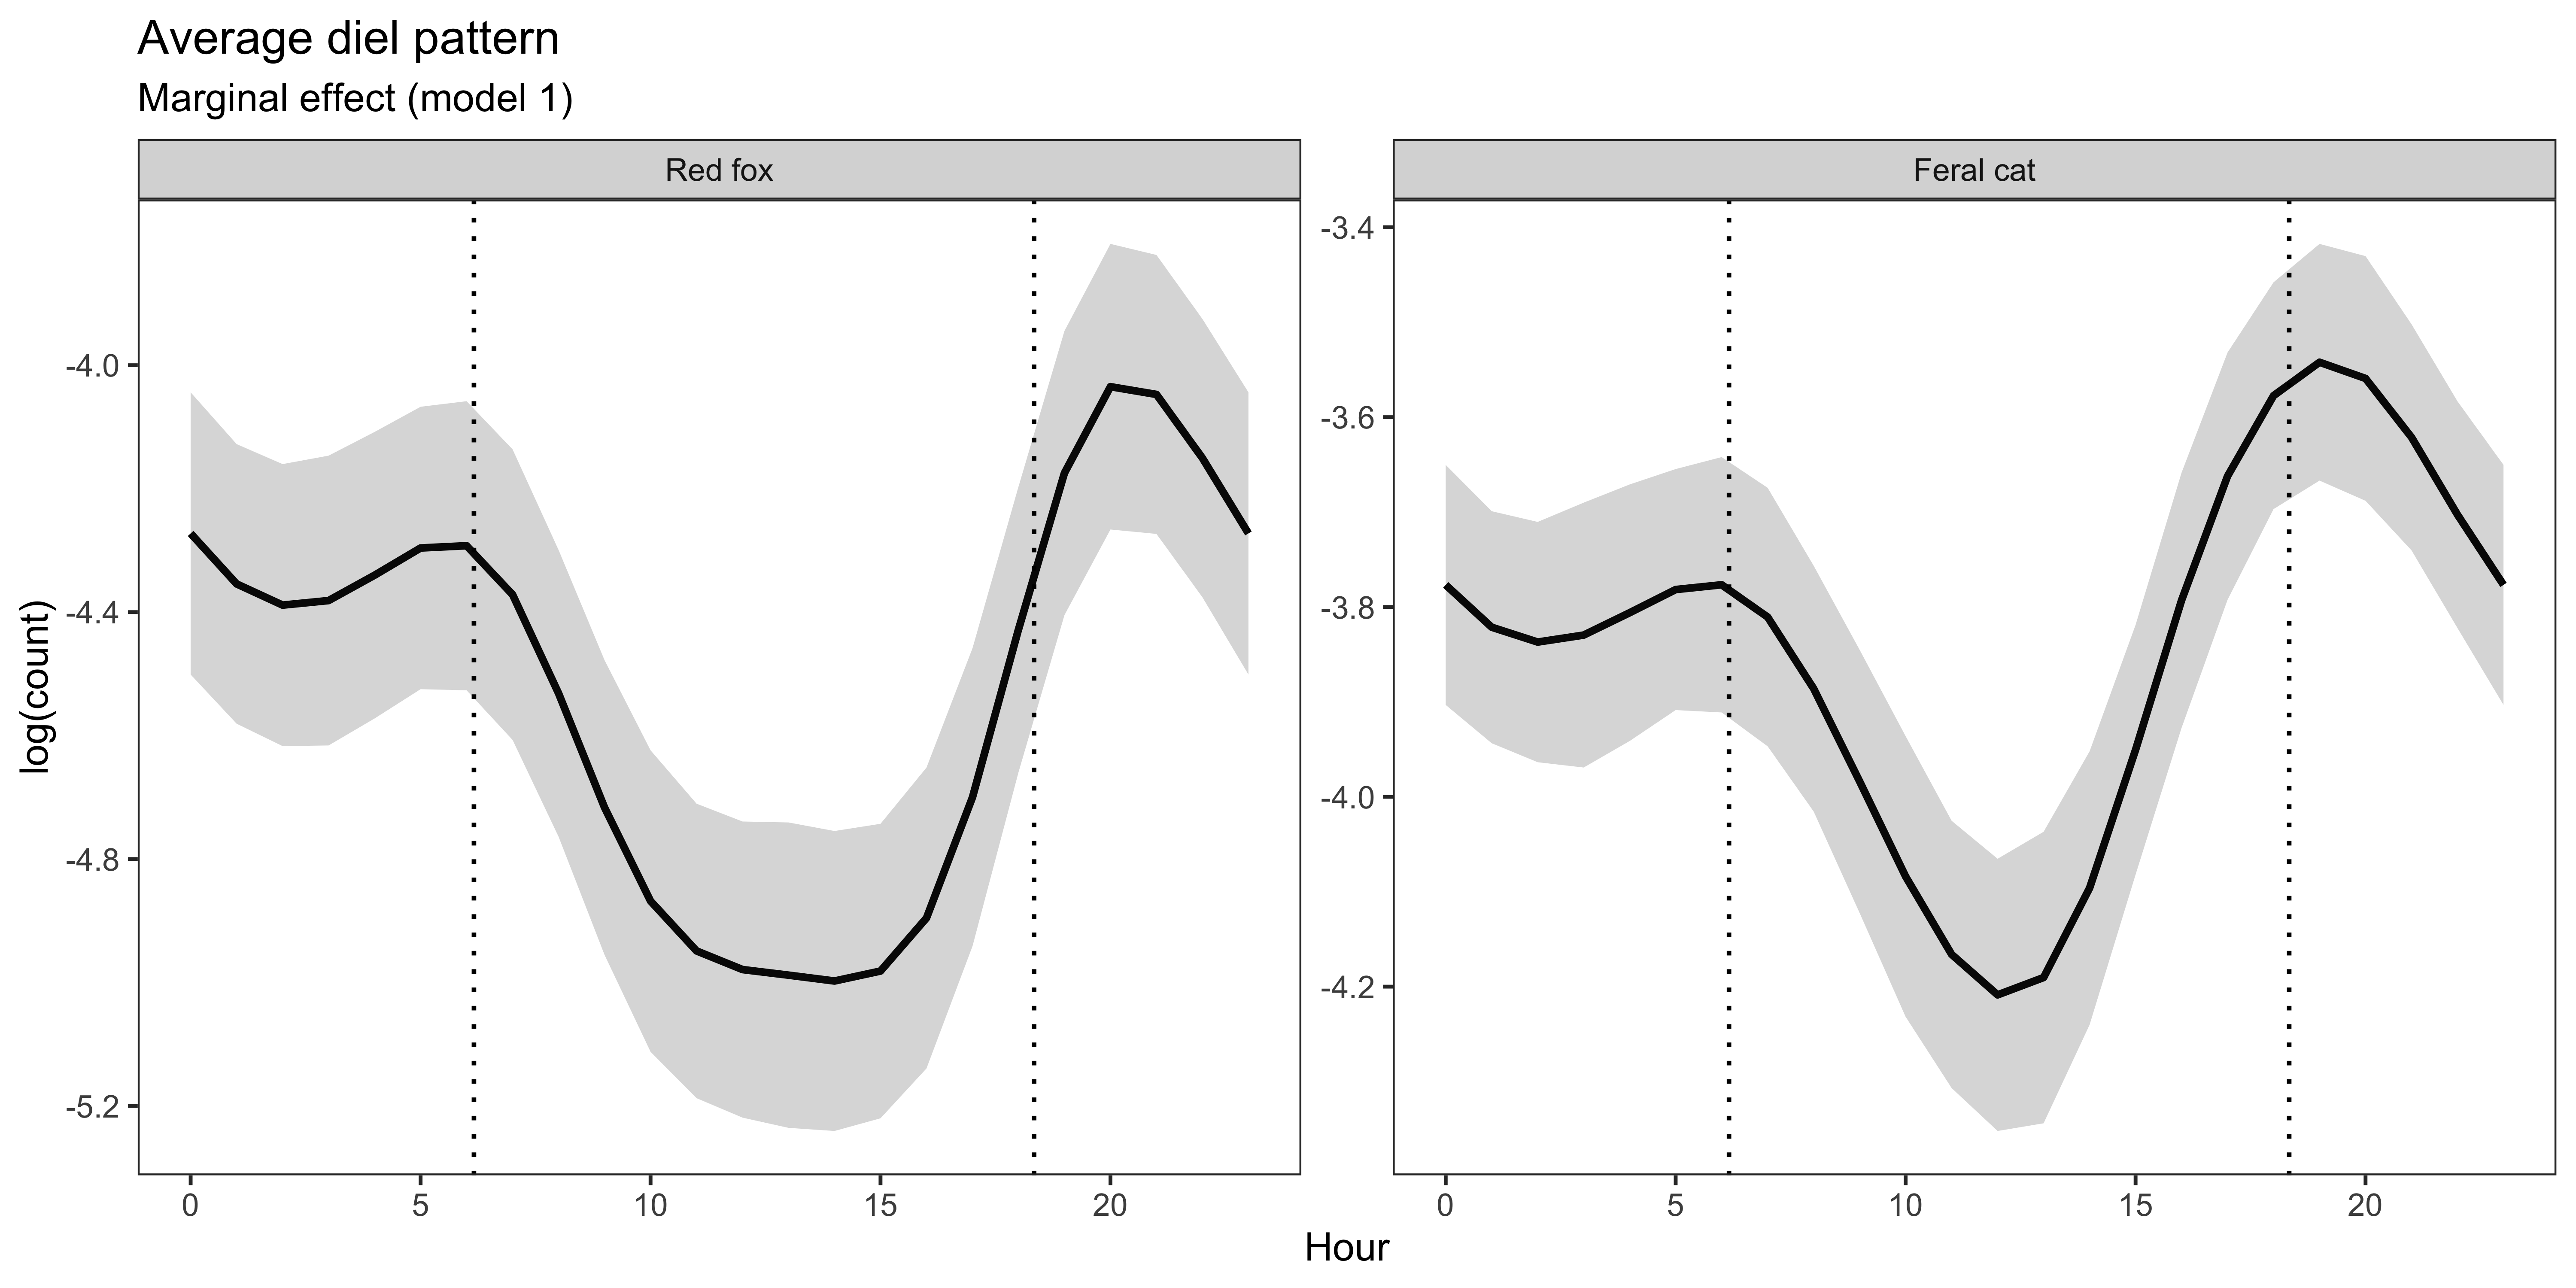
\includegraphics[width=1\linewidth]{../figs/avg_diel_predator} 

}

\caption{Marginal effect of time (model 1) on predators across both study regions in south-west Victoria, Australia. White crosses depict unique camera-trap sites}\label{fig:diel-space-time-marginal}
\end{figure}

\newpage

\begin{center}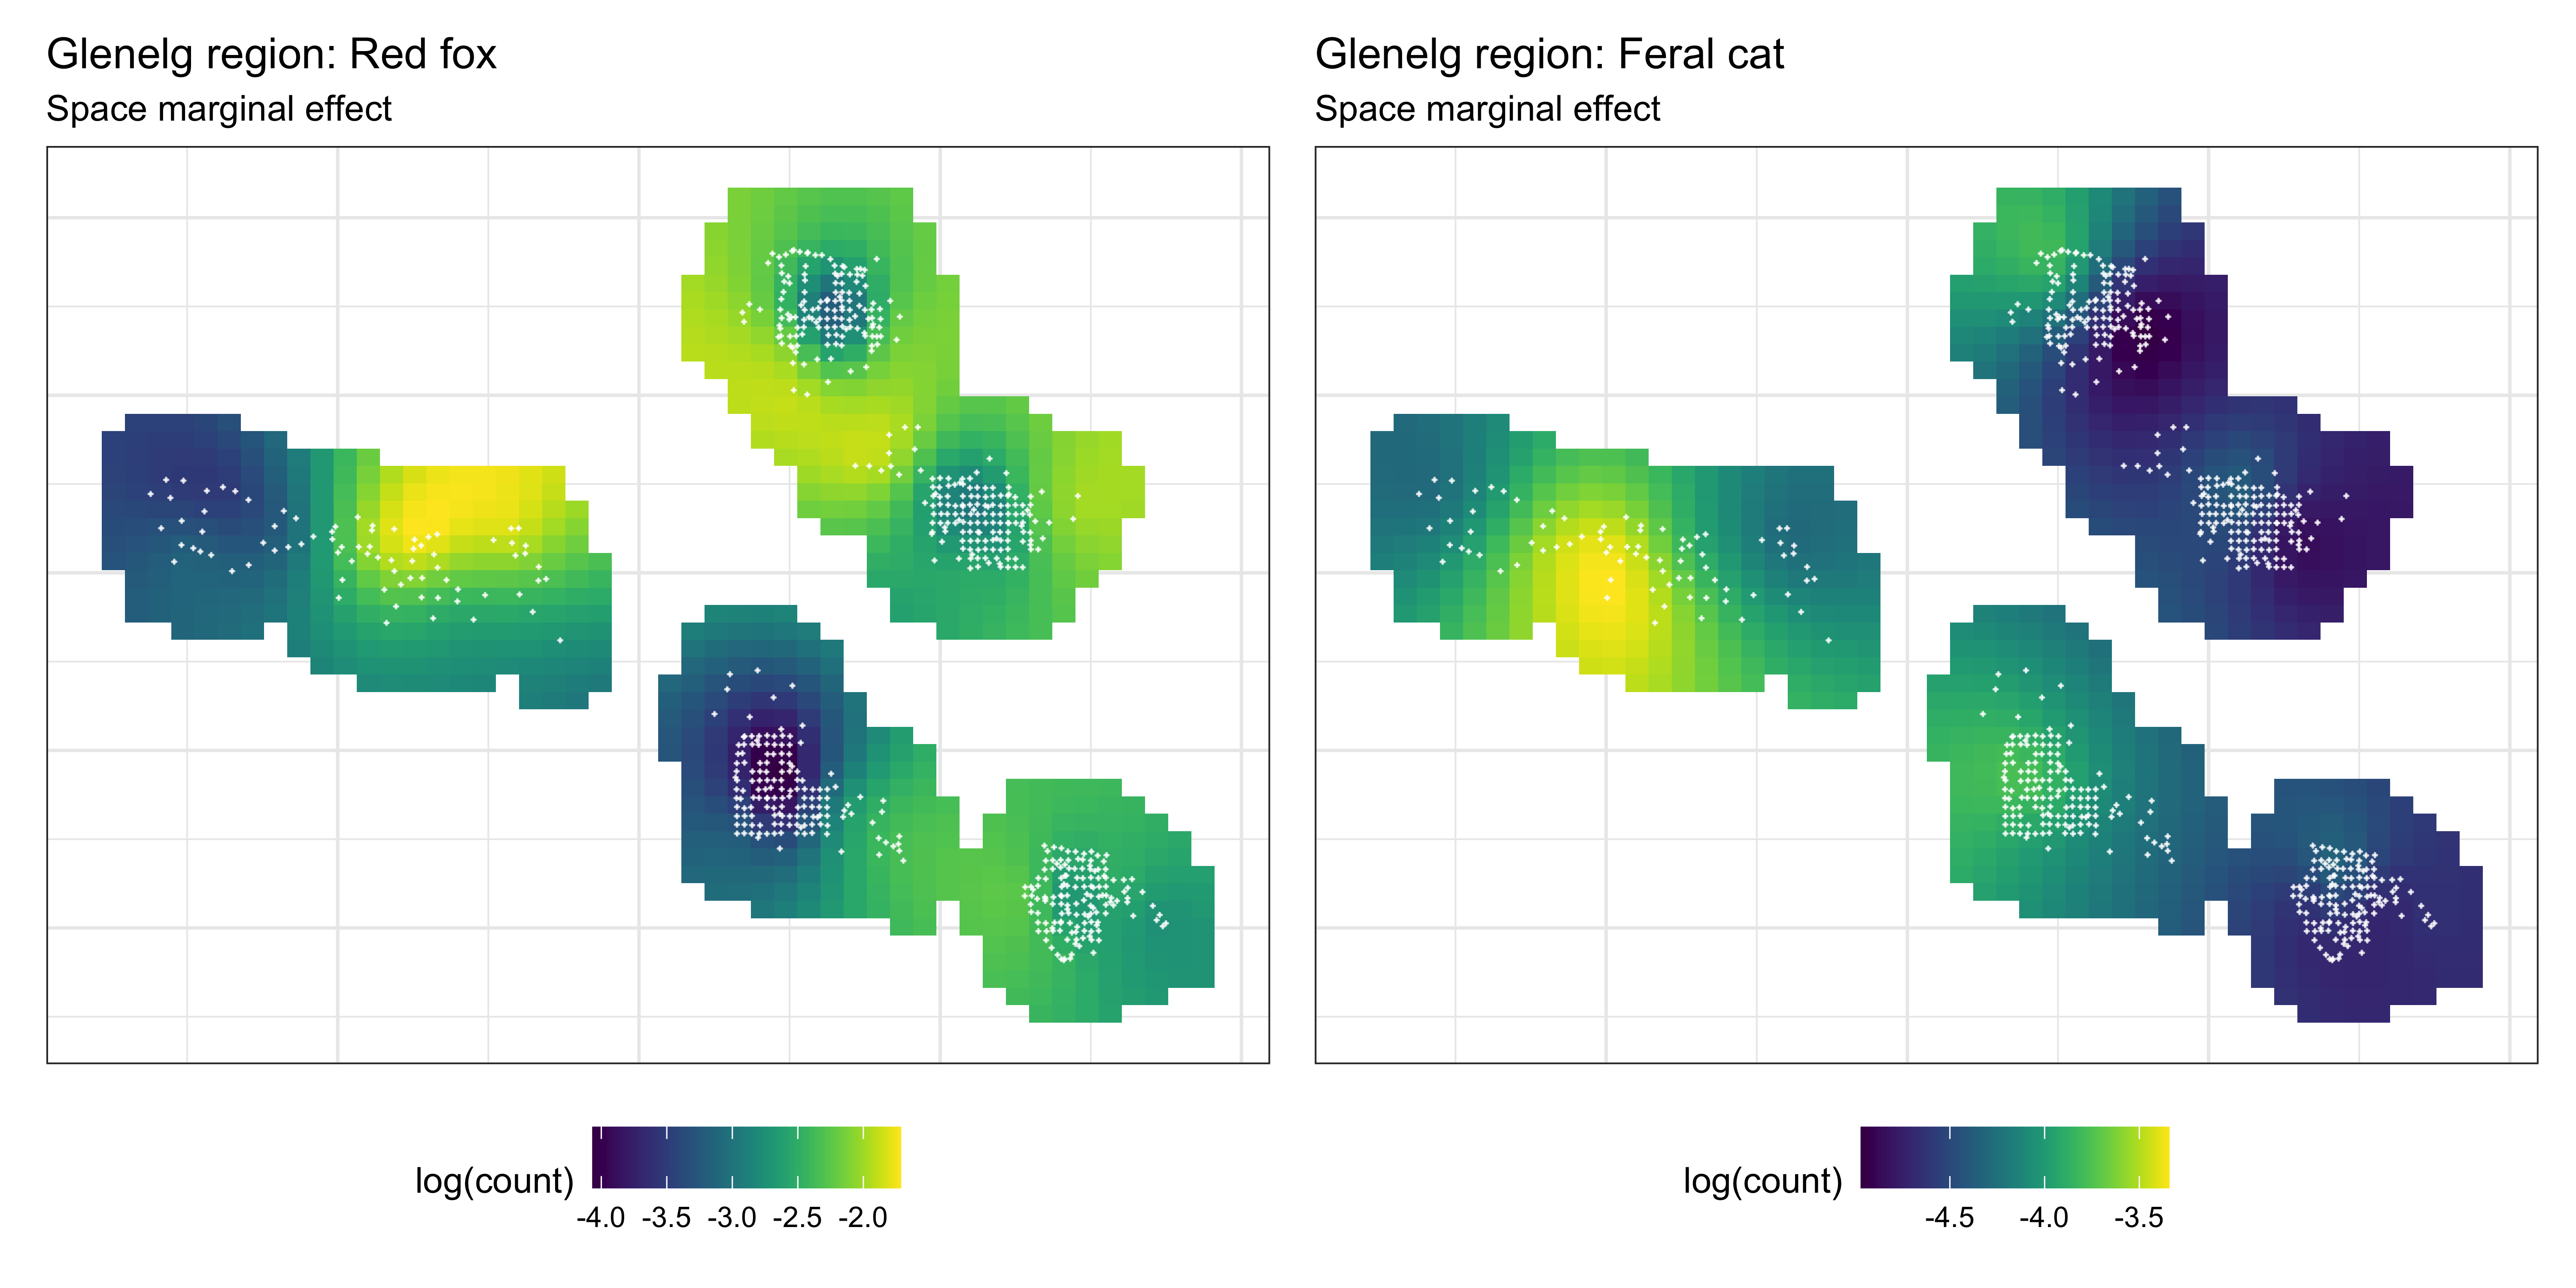
\includegraphics[width=1\linewidth]{../figs/sp_marginal_g} \end{center}

\begin{figure}

{\centering 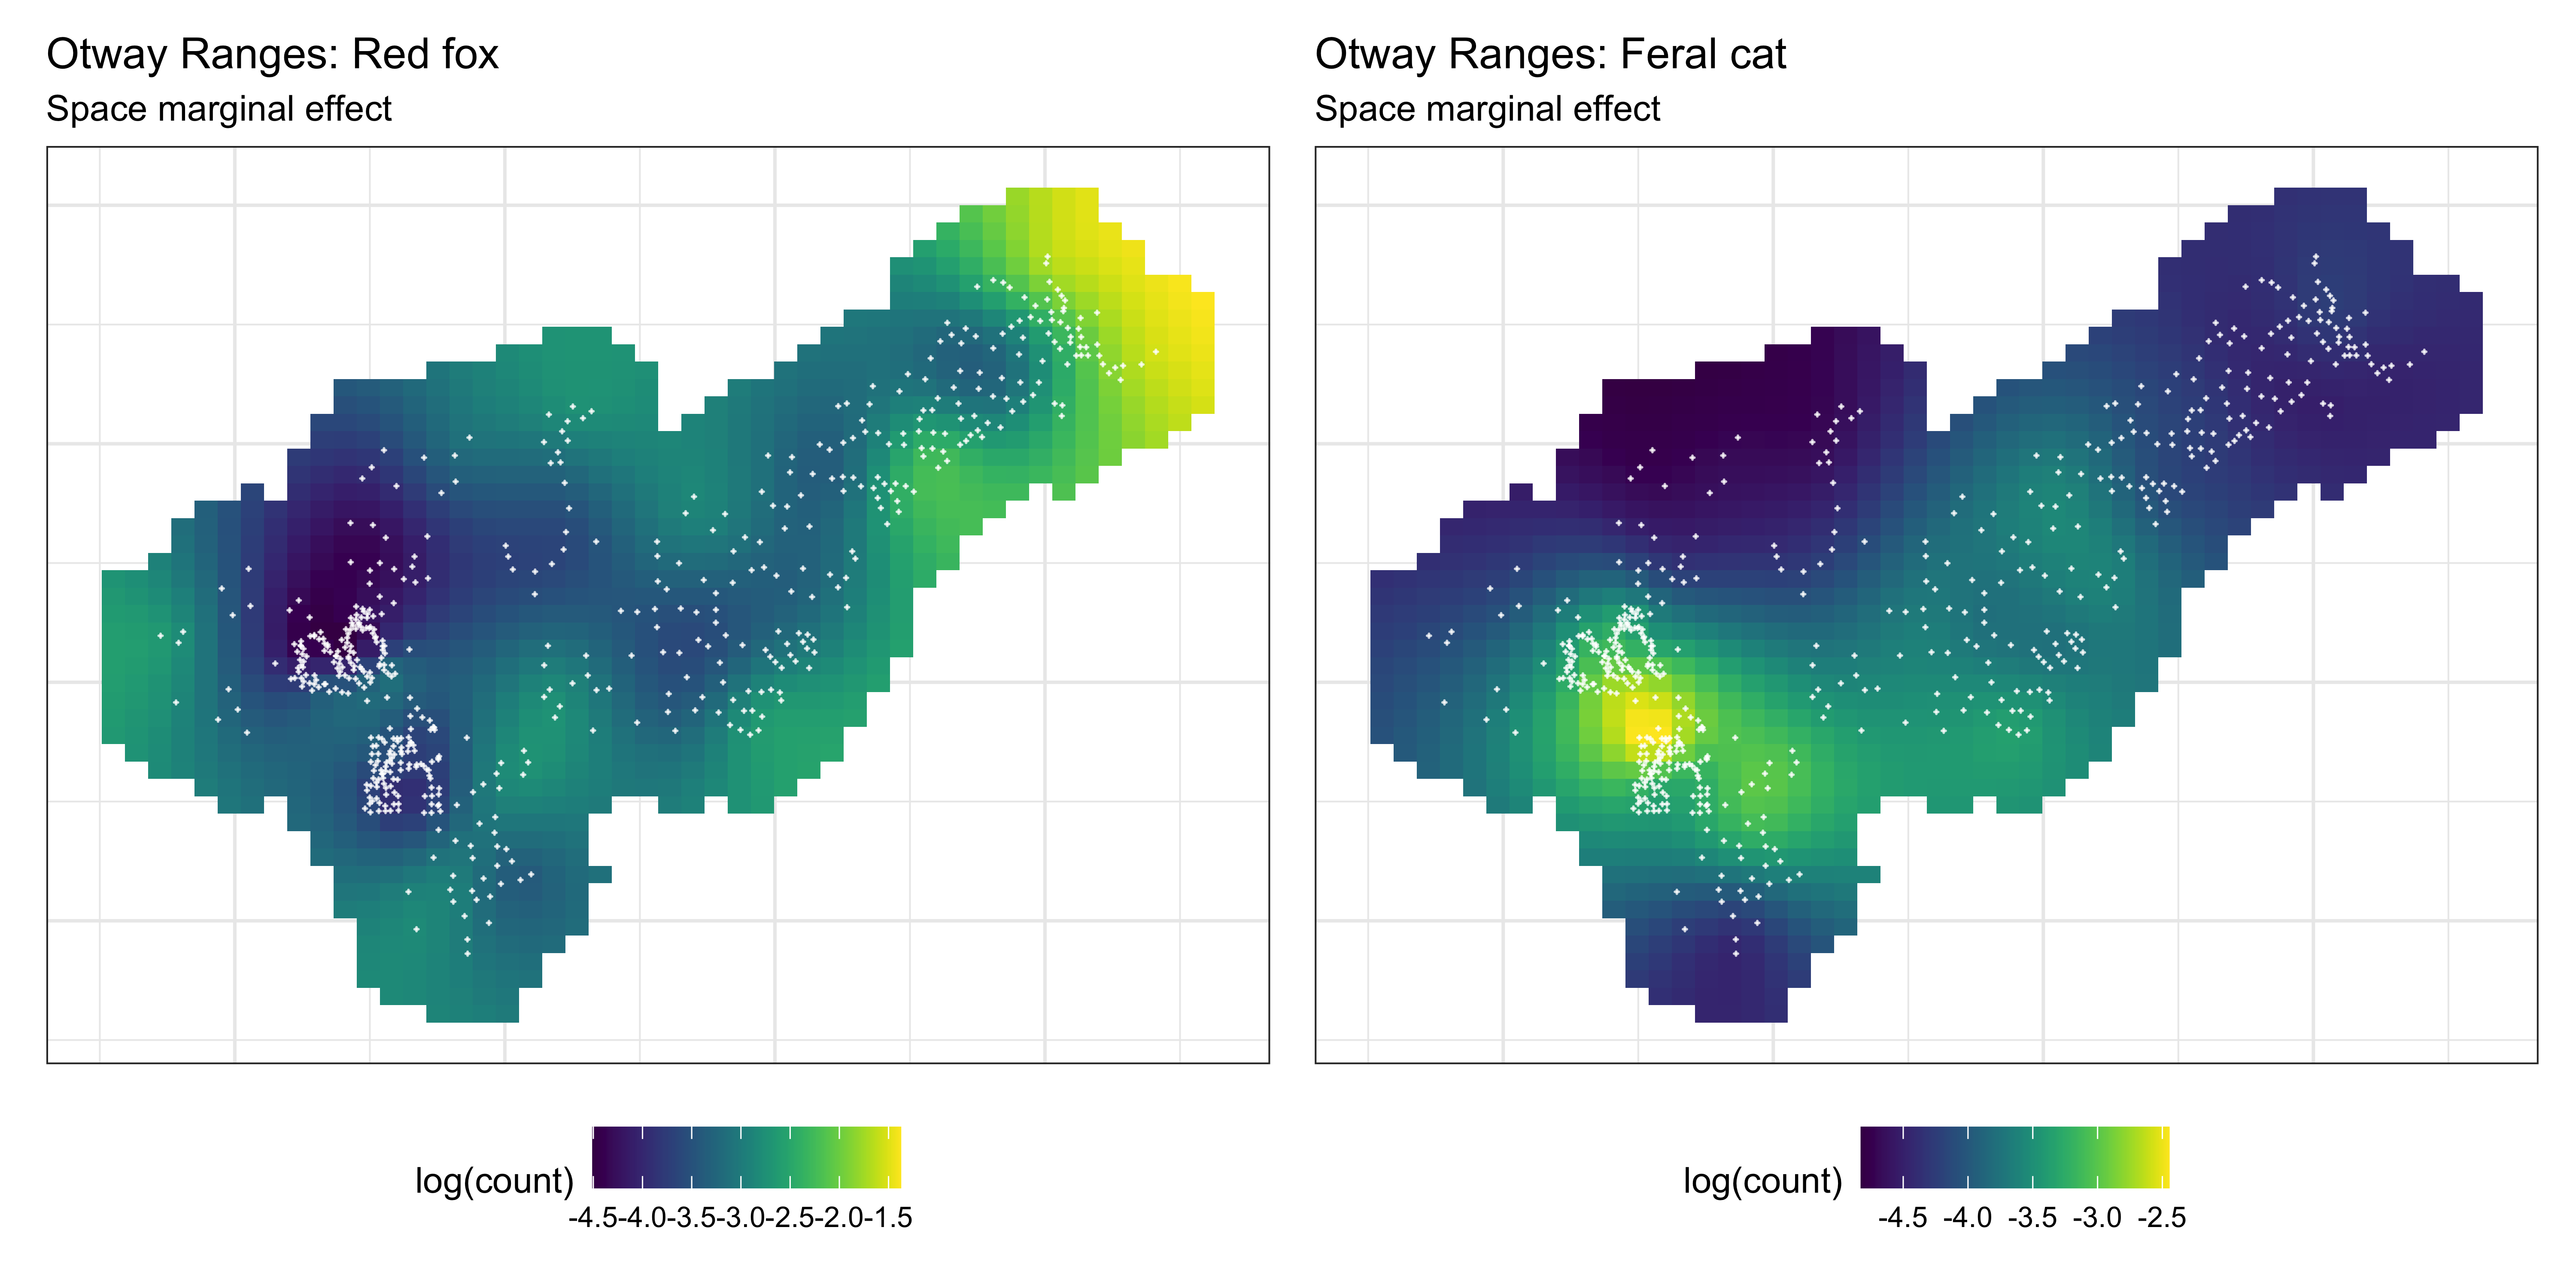
\includegraphics[width=1\linewidth]{../figs/sp_marginal_o} 

}

\caption{Marginal effect of space on predators across south-west Victoria, Australia (model 1). White crosses depict unique camera-trap sites}\label{fig:diel-space-time-marginal-o}
\end{figure}

\newpage

\begin{figure}

{\centering 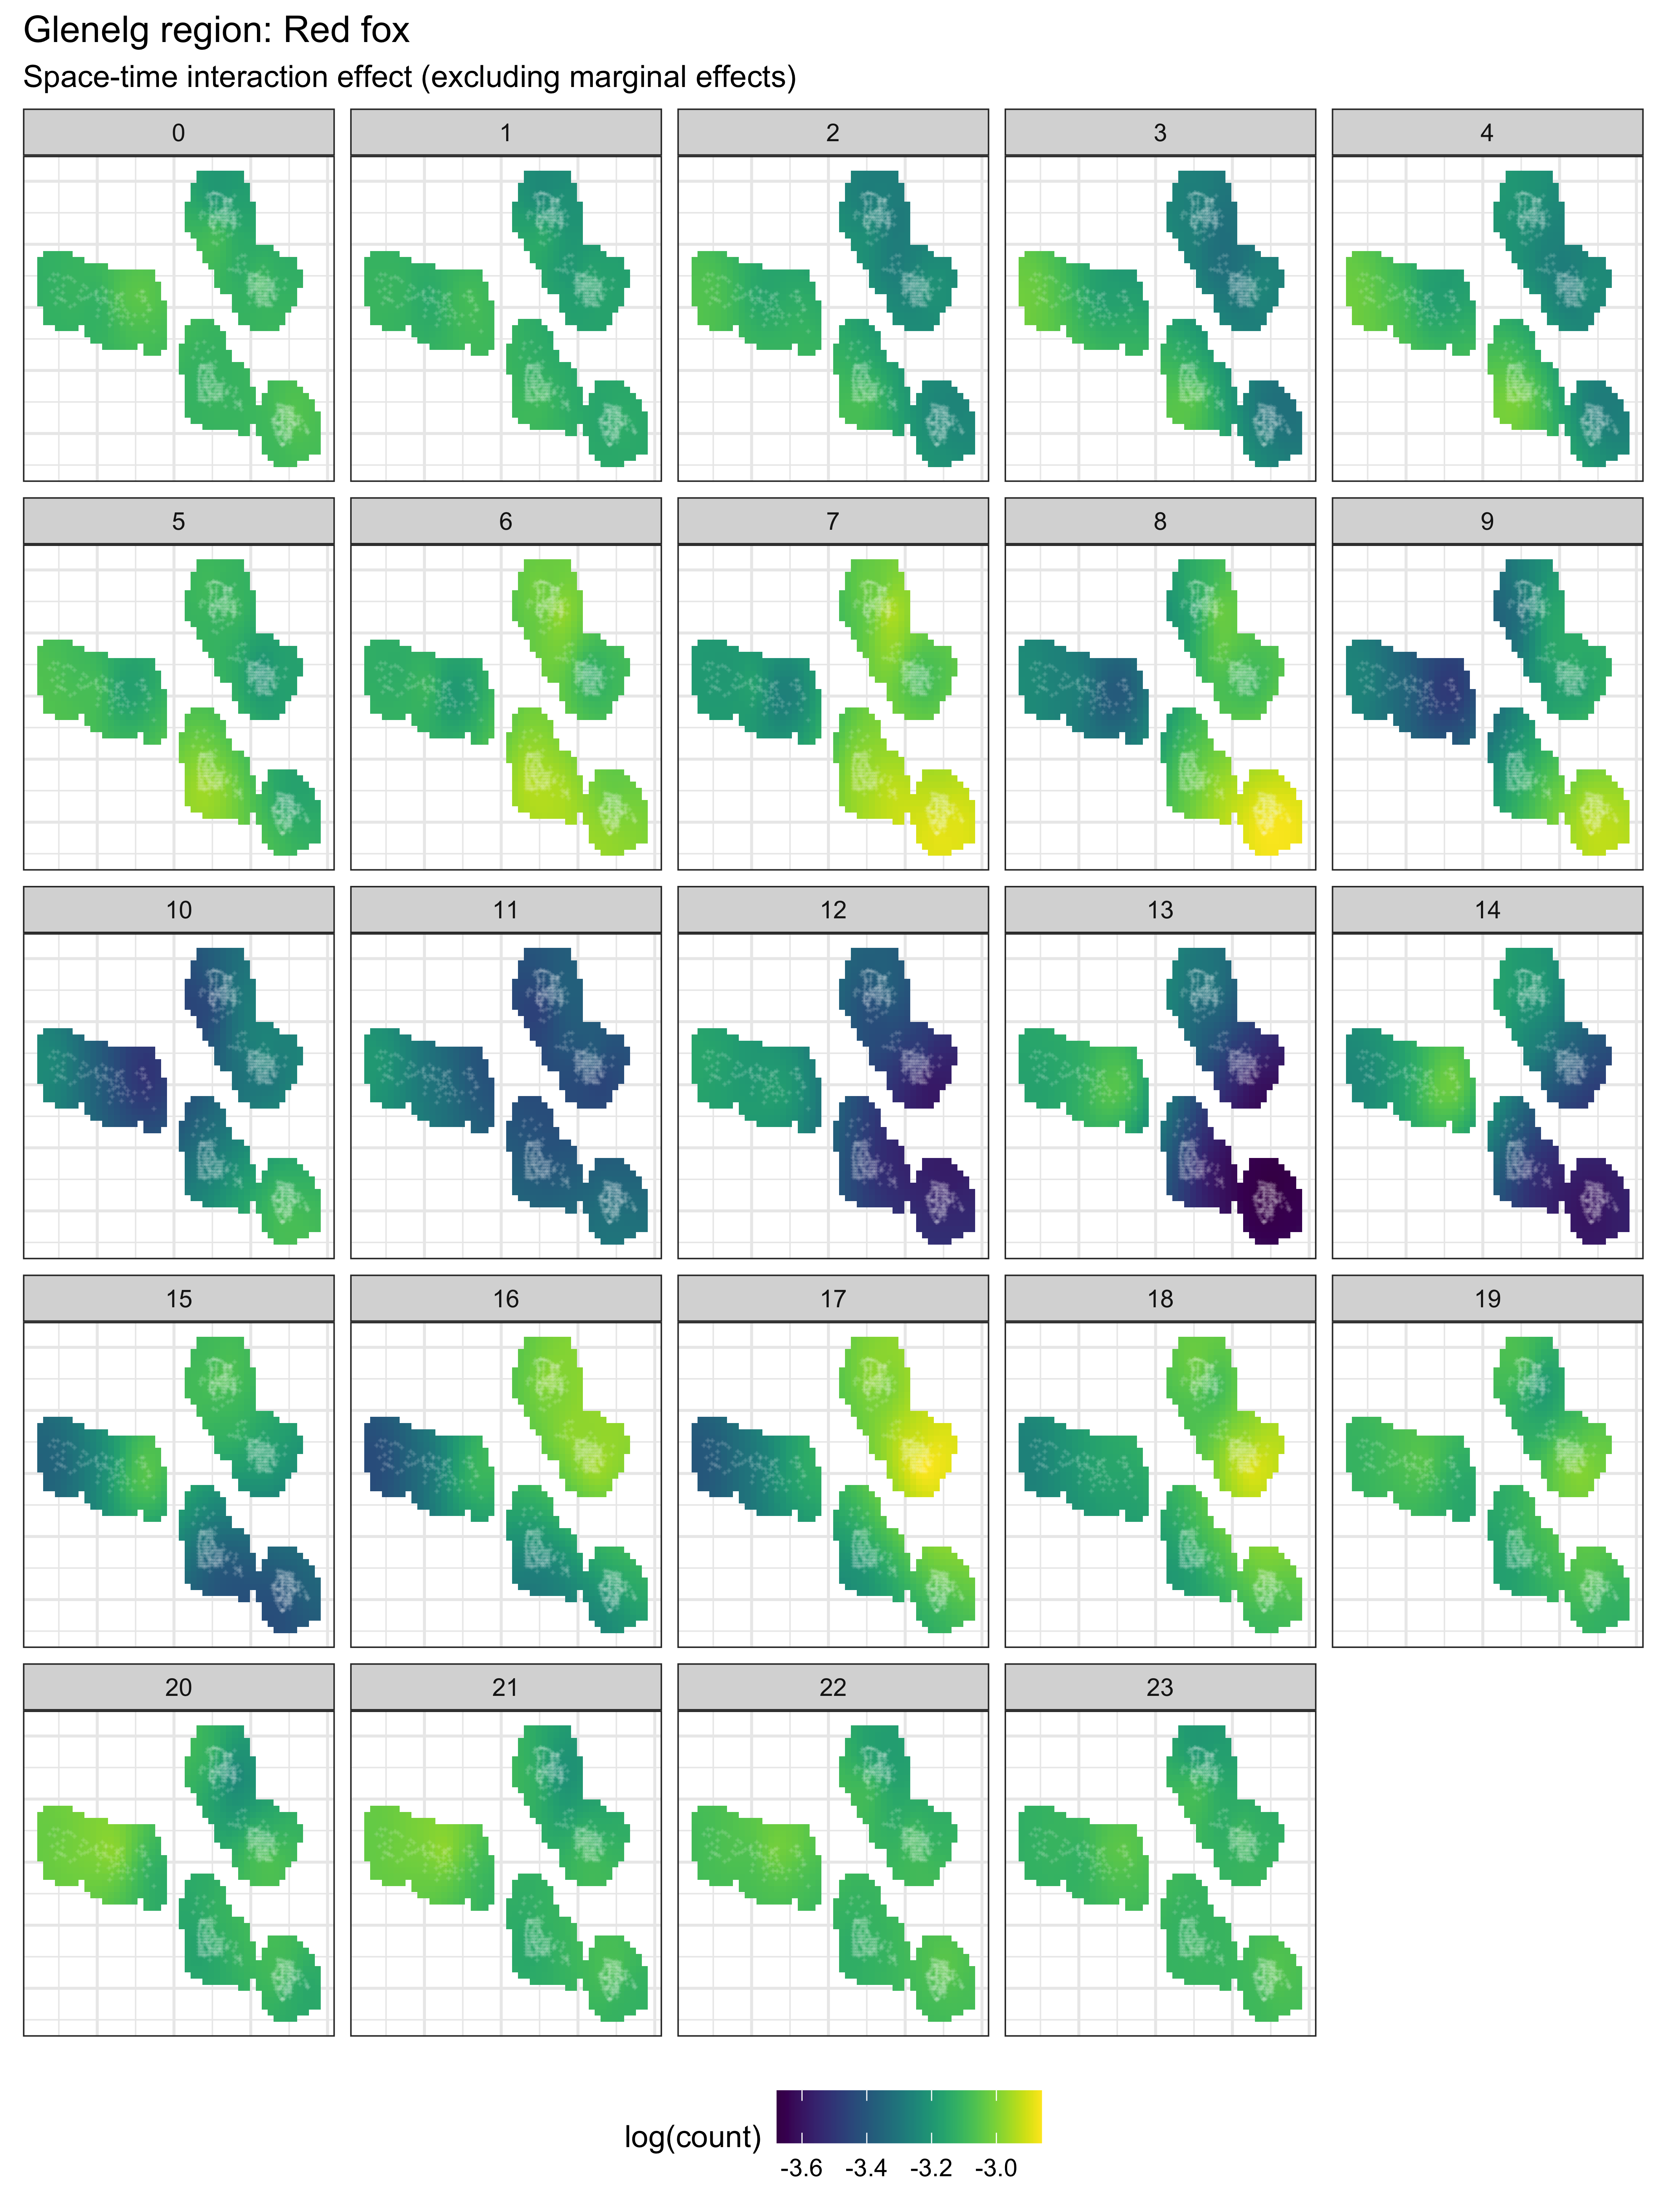
\includegraphics[width=1\linewidth]{../figs/spte_diff_avg_g_fox} 

}

\caption{Interaction effect of space-time on feral cat \textit{Felis catus} activity across each hour of the day (0 - 23) in the Glenelg region, Australia (model 1). White crosses depict unique camera-trap sites. }\label{fig:diel-st-int-g-fox}
\end{figure}

\newpage

\begin{figure}

{\centering 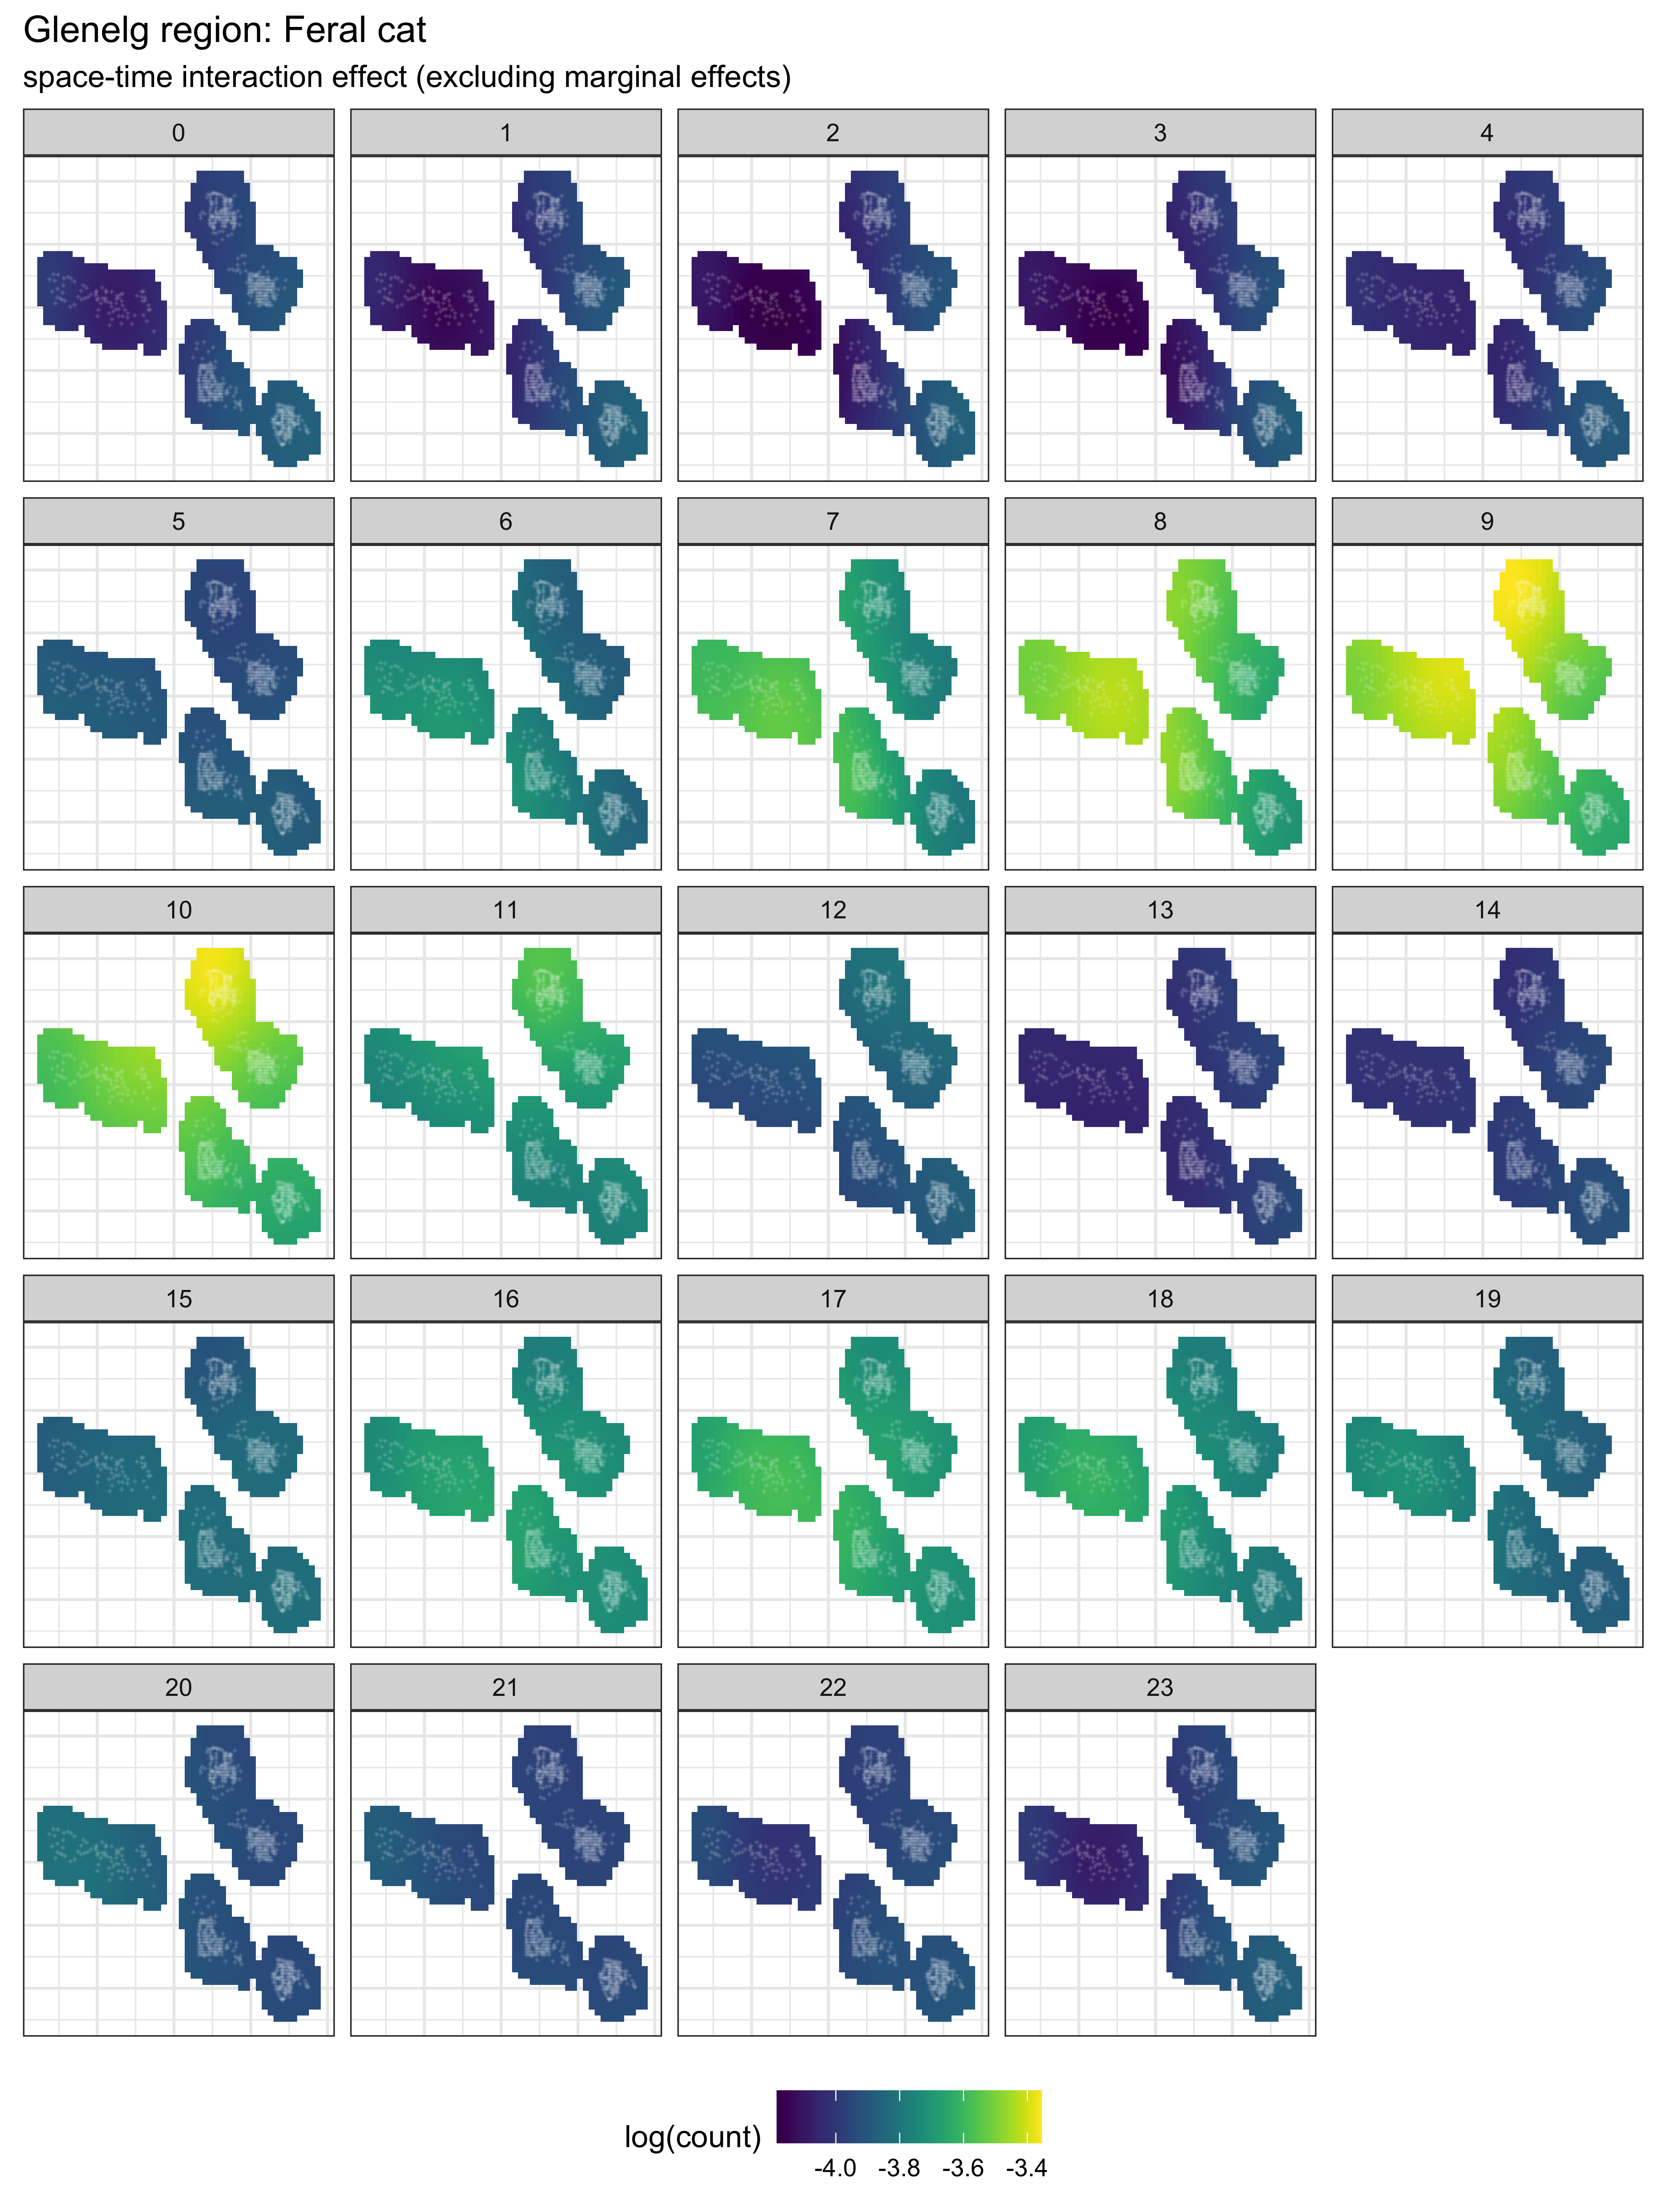
\includegraphics[width=1\linewidth]{../figs/spte_diff_avg_g_cat} 

}

\caption{Interaction effect of space-time on feral cat \textit{Felis catus} activity across each hour of the day (0 - 23) in the Glenelg region, Australia (model 1). White crosses depict unique camera-trap sites. }\label{fig:diel-st-int-g-cat}
\end{figure}

\newpage

\begin{figure}

{\centering 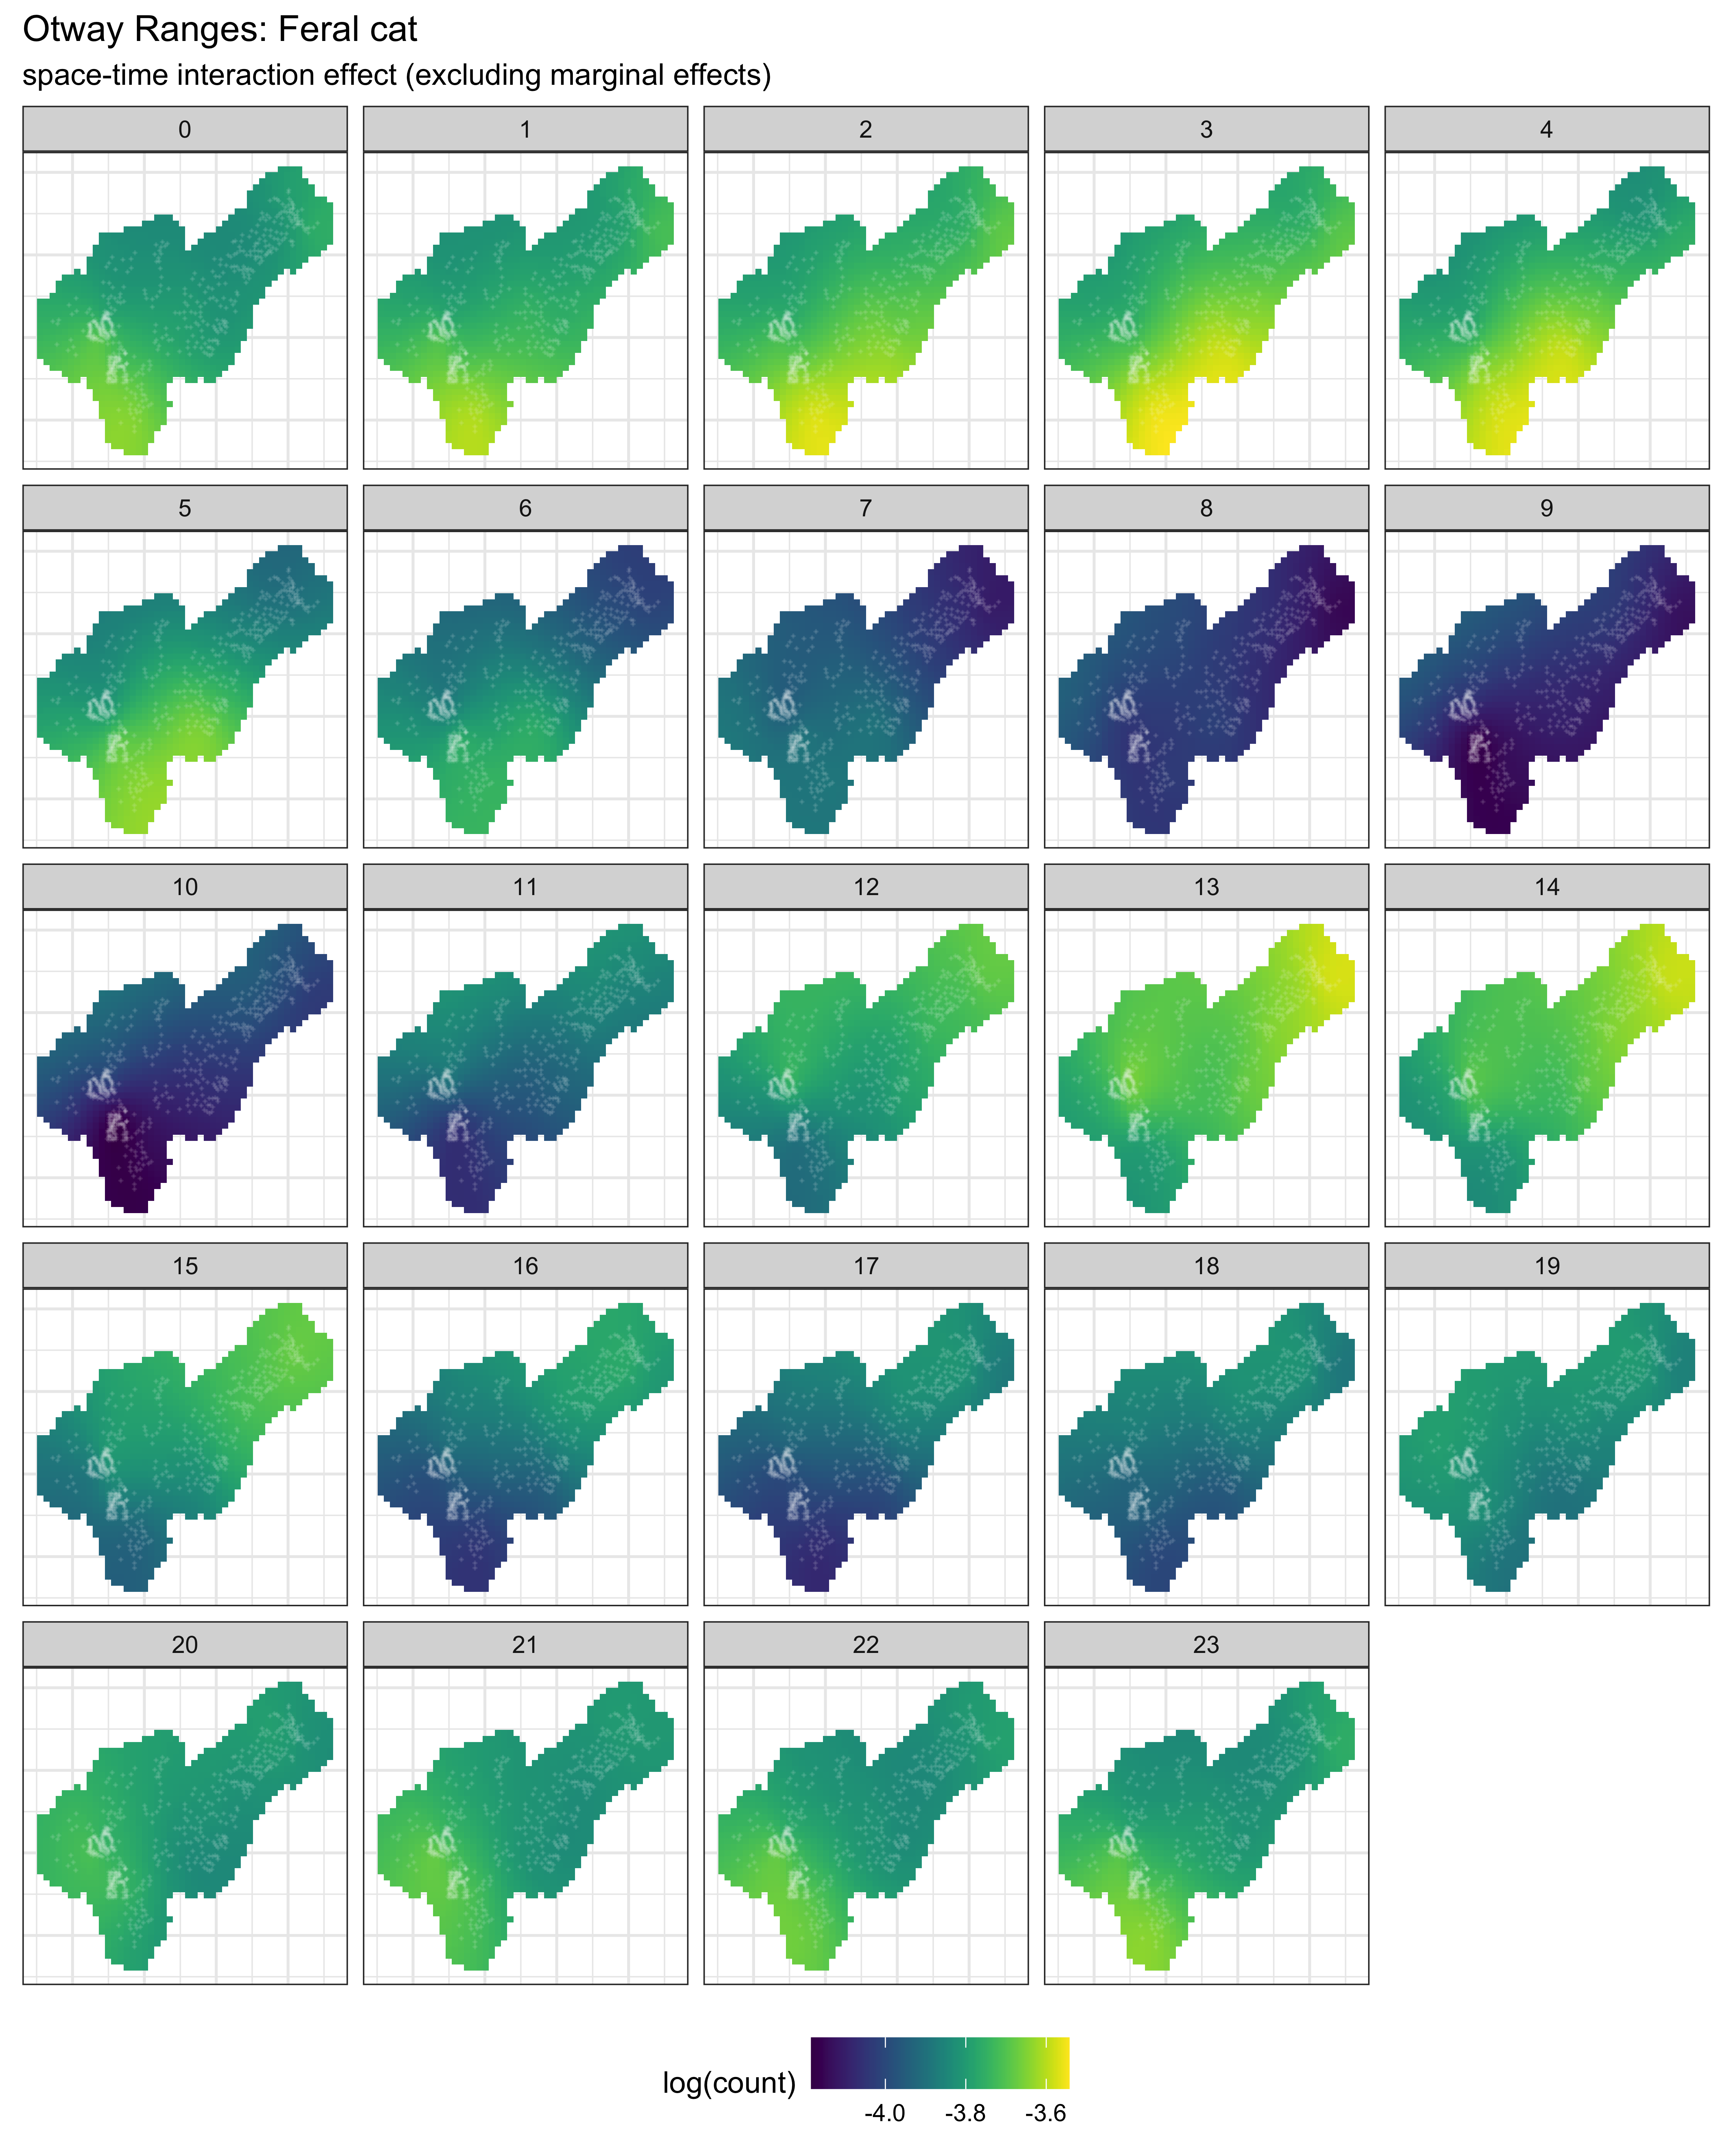
\includegraphics[width=1\linewidth]{../figs/spte_diff_avg_o_cat} 

}

\caption{Interaction effect of space-time on feral cat \textit{Felis catus} activity across each hour of the day (0 - 23) in the Otway Ranges, Australia (model 1). White crosses depict unique camera-trap sites. }\label{fig:diel-st-int-o-cat}
\end{figure}

\newpage

\begin{figure}

{\centering 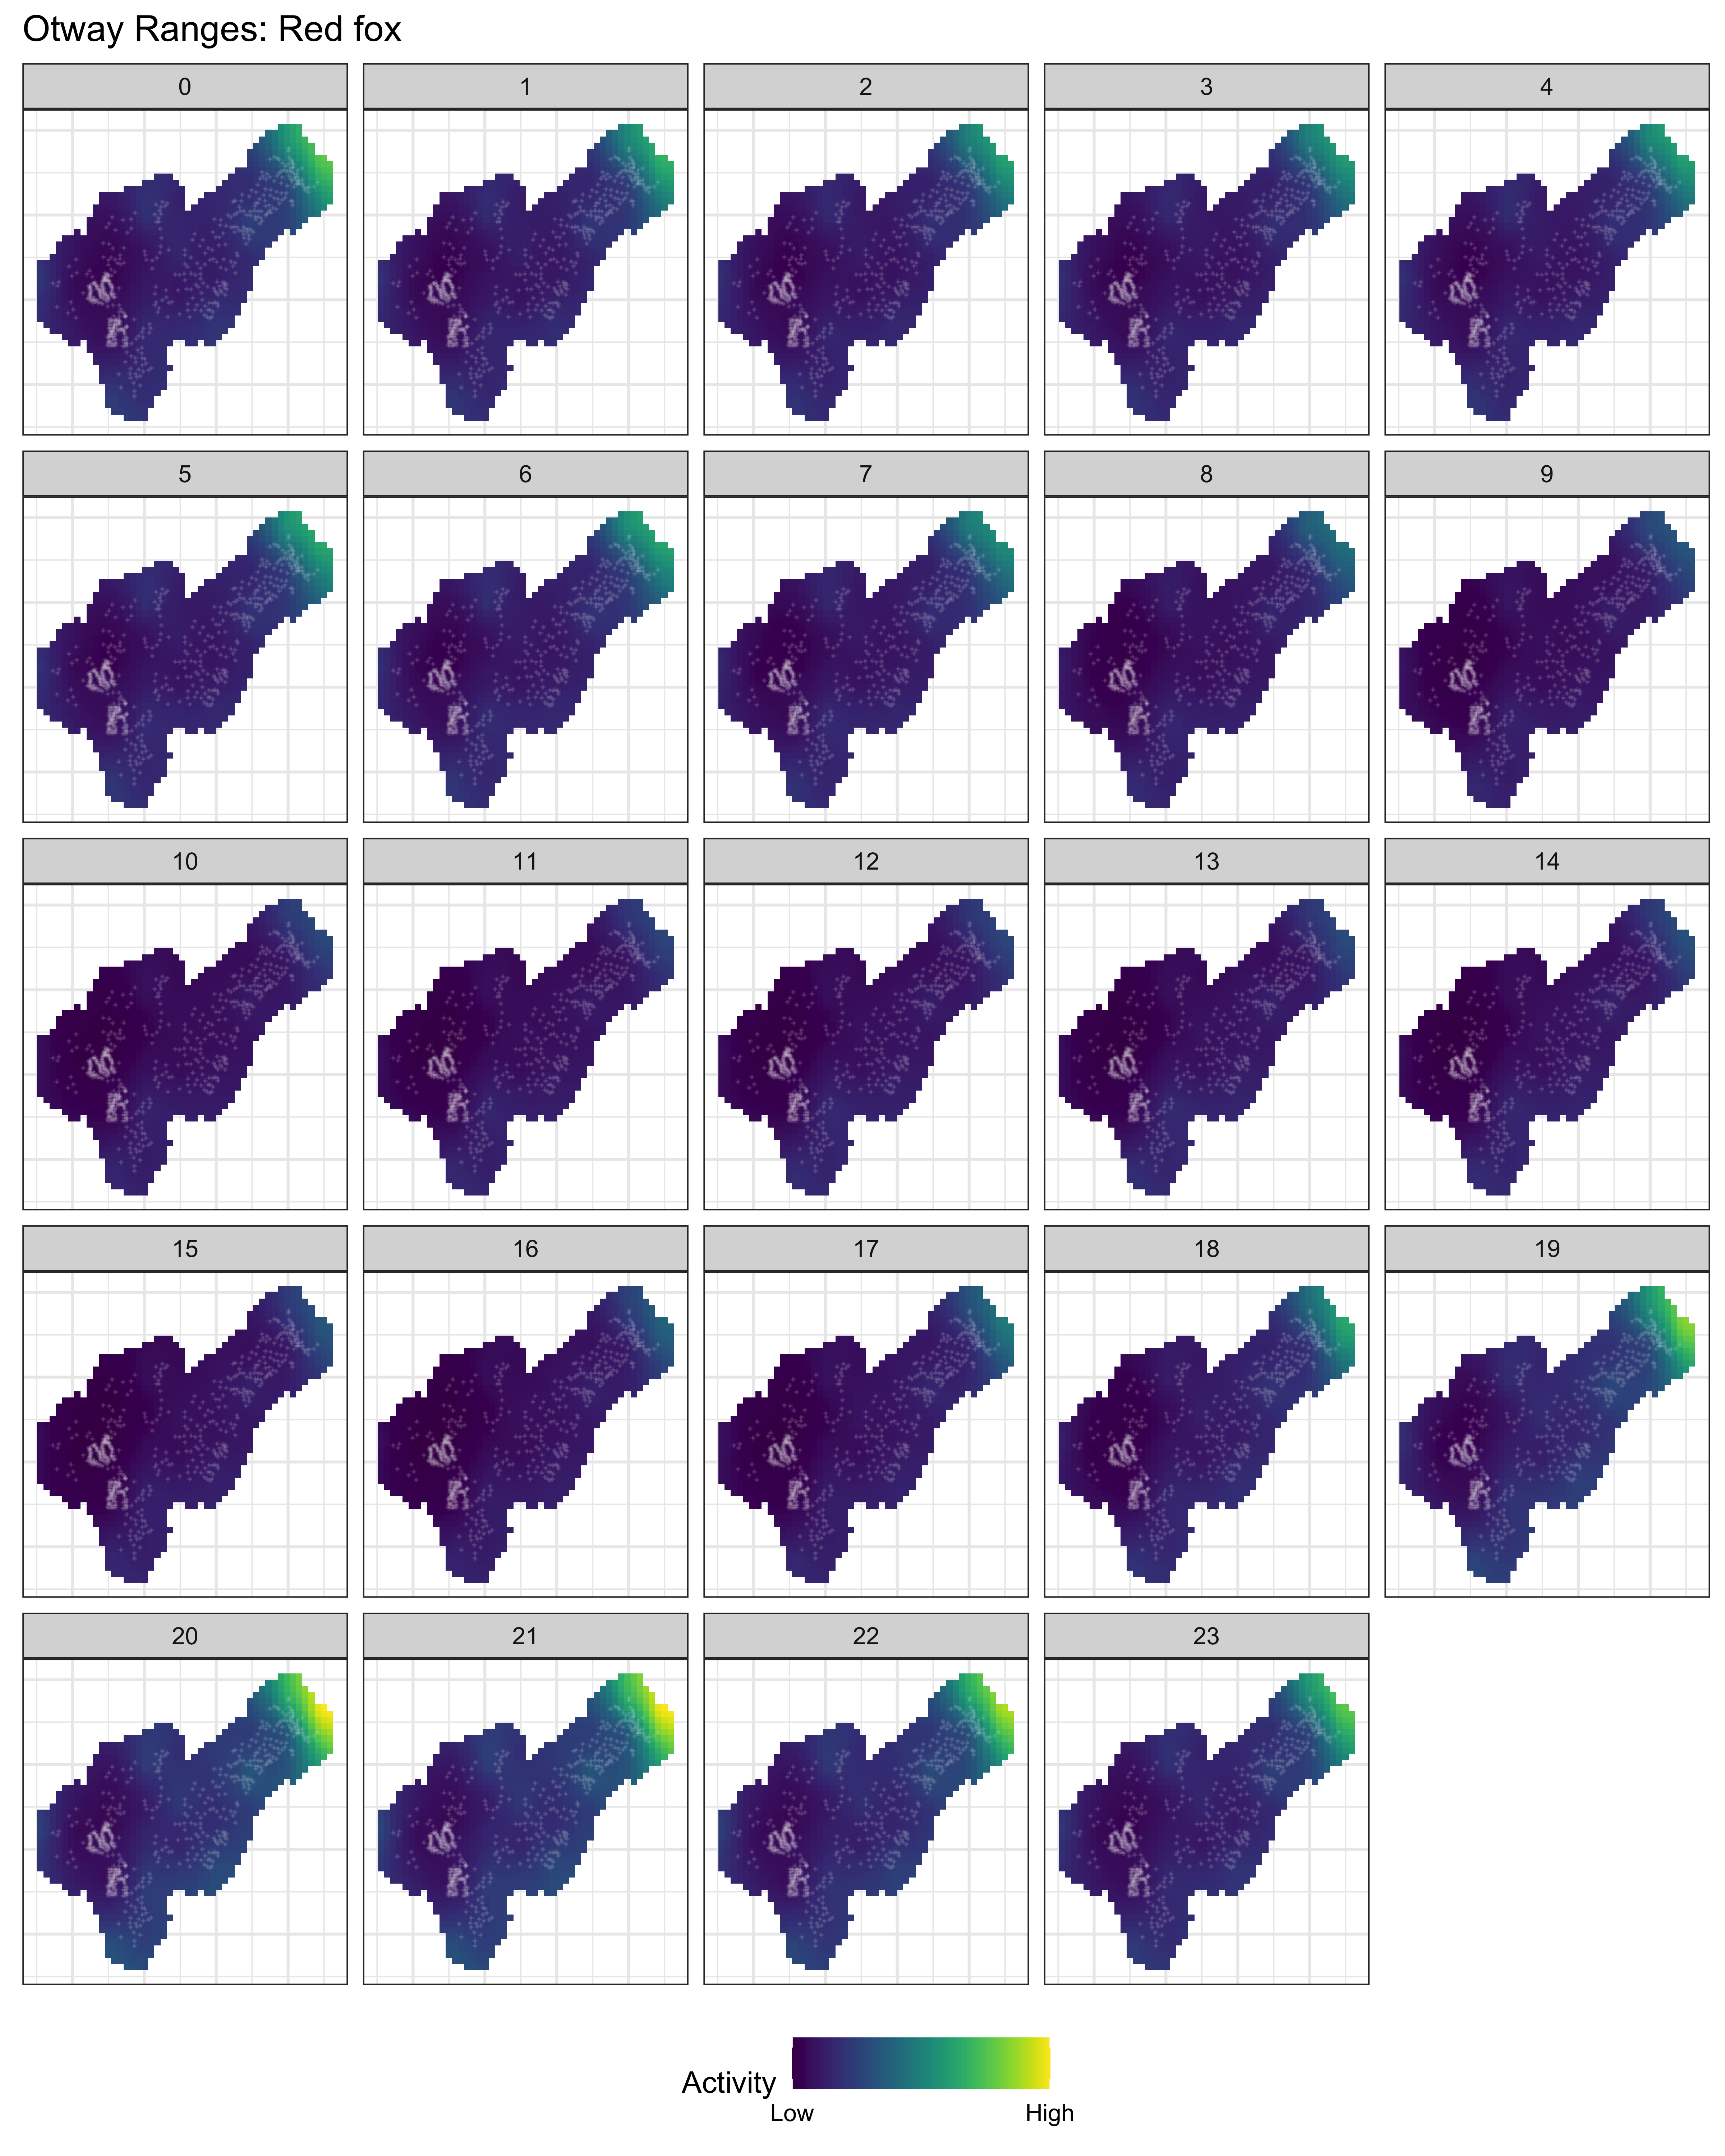
\includegraphics[width=1\linewidth]{../figs/spte_facet_o_fox} 

}

\caption{Overall spatial activity of red foxes \textit{Vulpes vulpes} for each hour of the day (0 - 23) in the Glenelg region, Australia (model 1). White crosses depict unique camera-trap sites}\label{fig:diel-space-g-fox}
\end{figure}

\newpage

\begin{figure}

{\centering 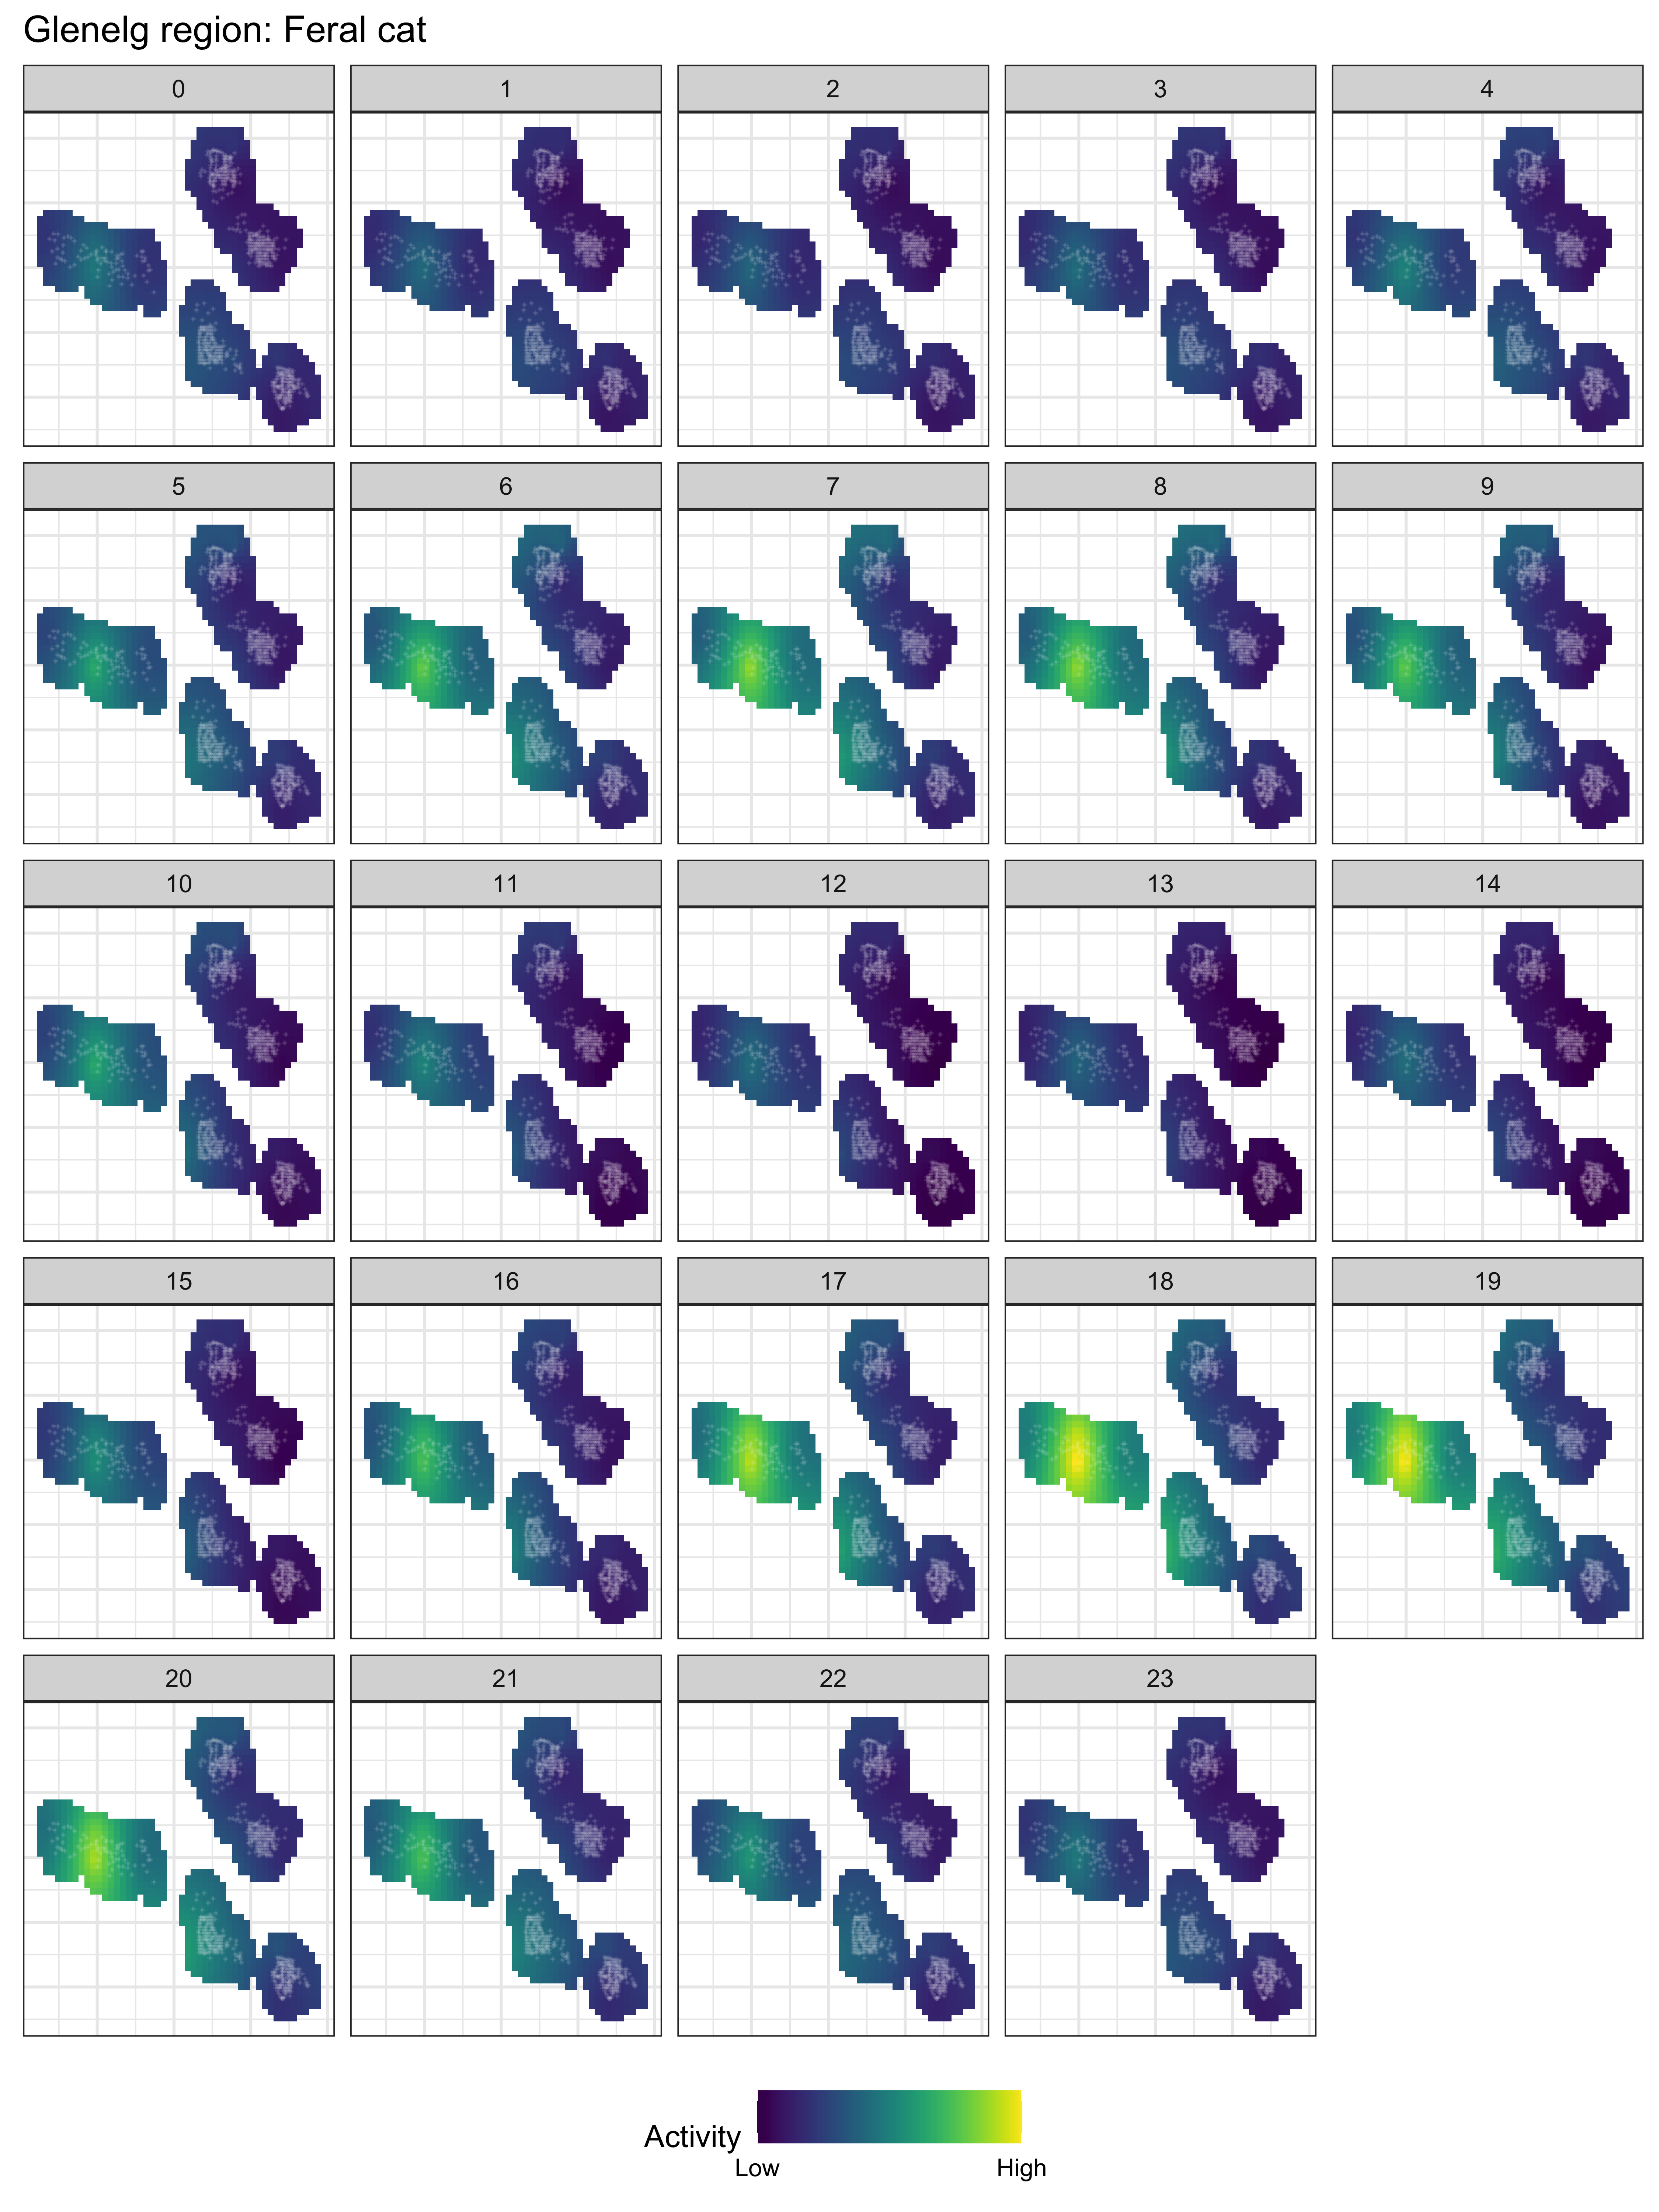
\includegraphics[width=1\linewidth]{../figs/spte_facet_g_cat} 

}

\caption{Overall spatial activity of feral cats \textit{Felis catus} for each hour of the day (0 - 23) in the Glenelg region, Australia (model 1). White crosses depict unique camera-trap sites}\label{fig:diel-space-g-cat}
\end{figure}

\newpage

\begin{figure}

{\centering 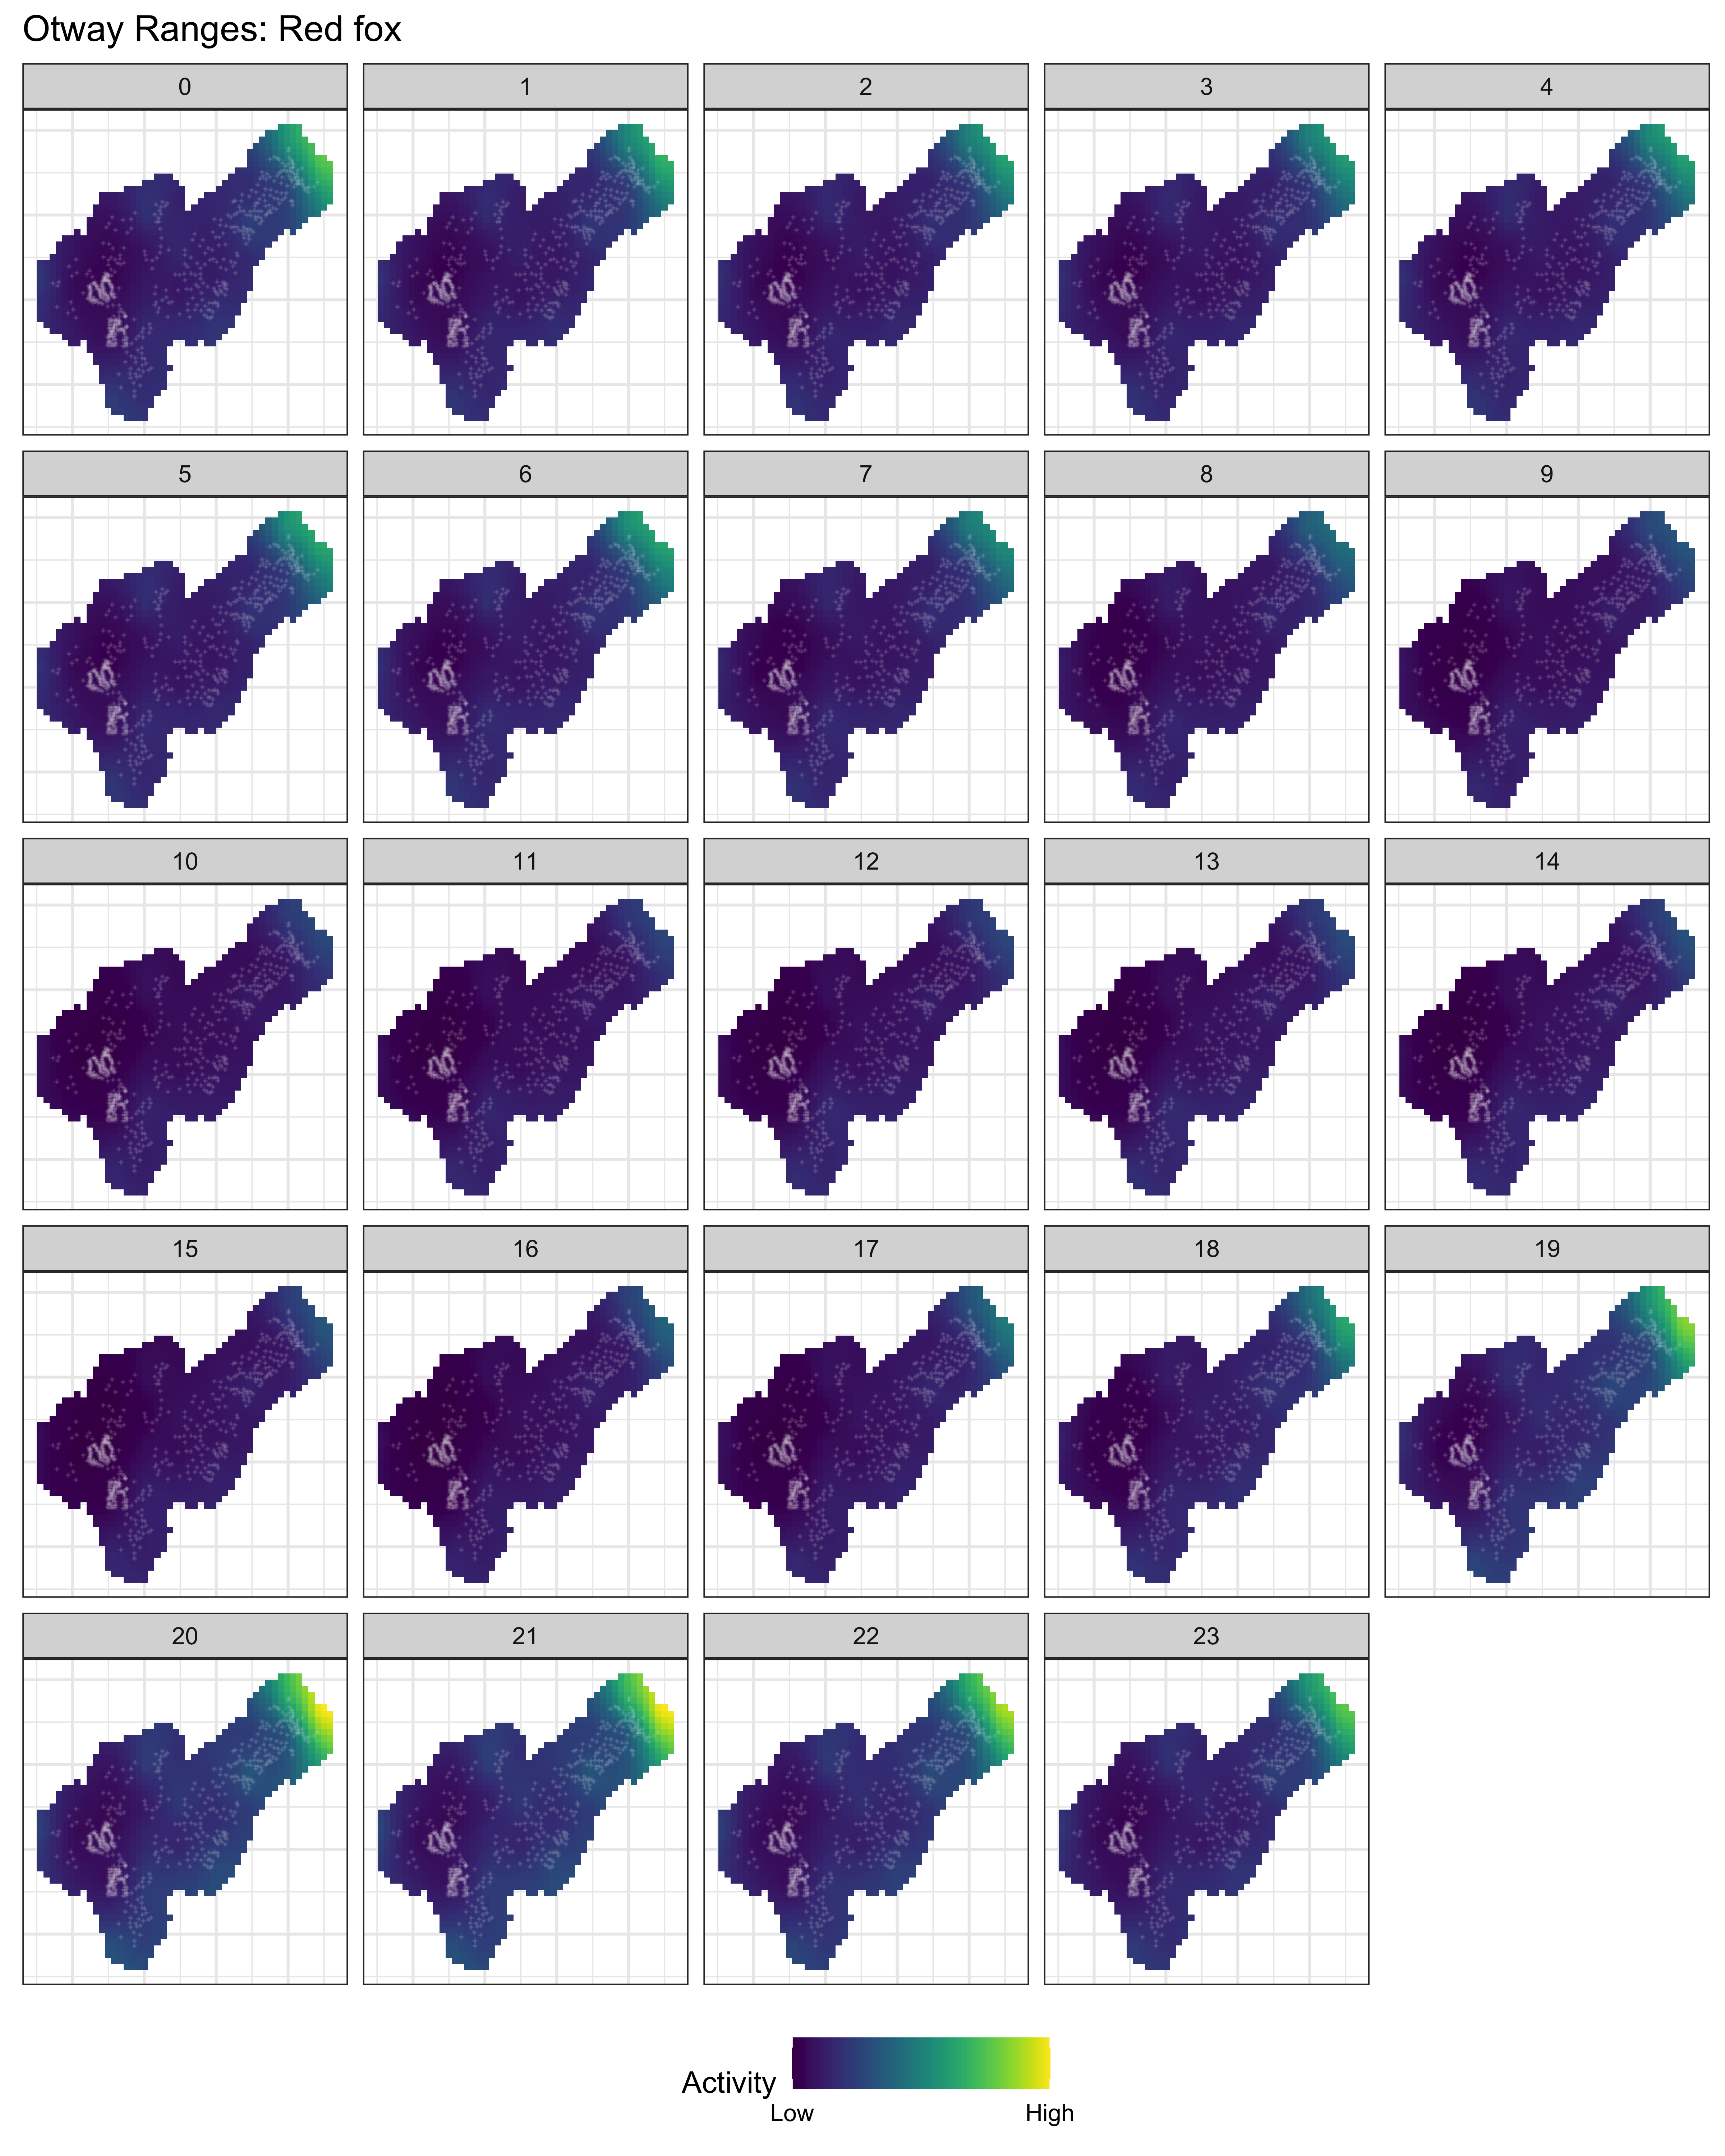
\includegraphics[width=1\linewidth]{../figs/spte_facet_o_fox} 

}

\caption{Overall spatial activity of red foxes \textit{Vulpes vulpes} for each hour of the day (0 - 23) in the Otway Ranges, Australia (model 1). White crosses depict unique camera-trap sites}\label{fig:diel-space-o-fox}
\end{figure}

\newpage

\begin{figure}

{\centering 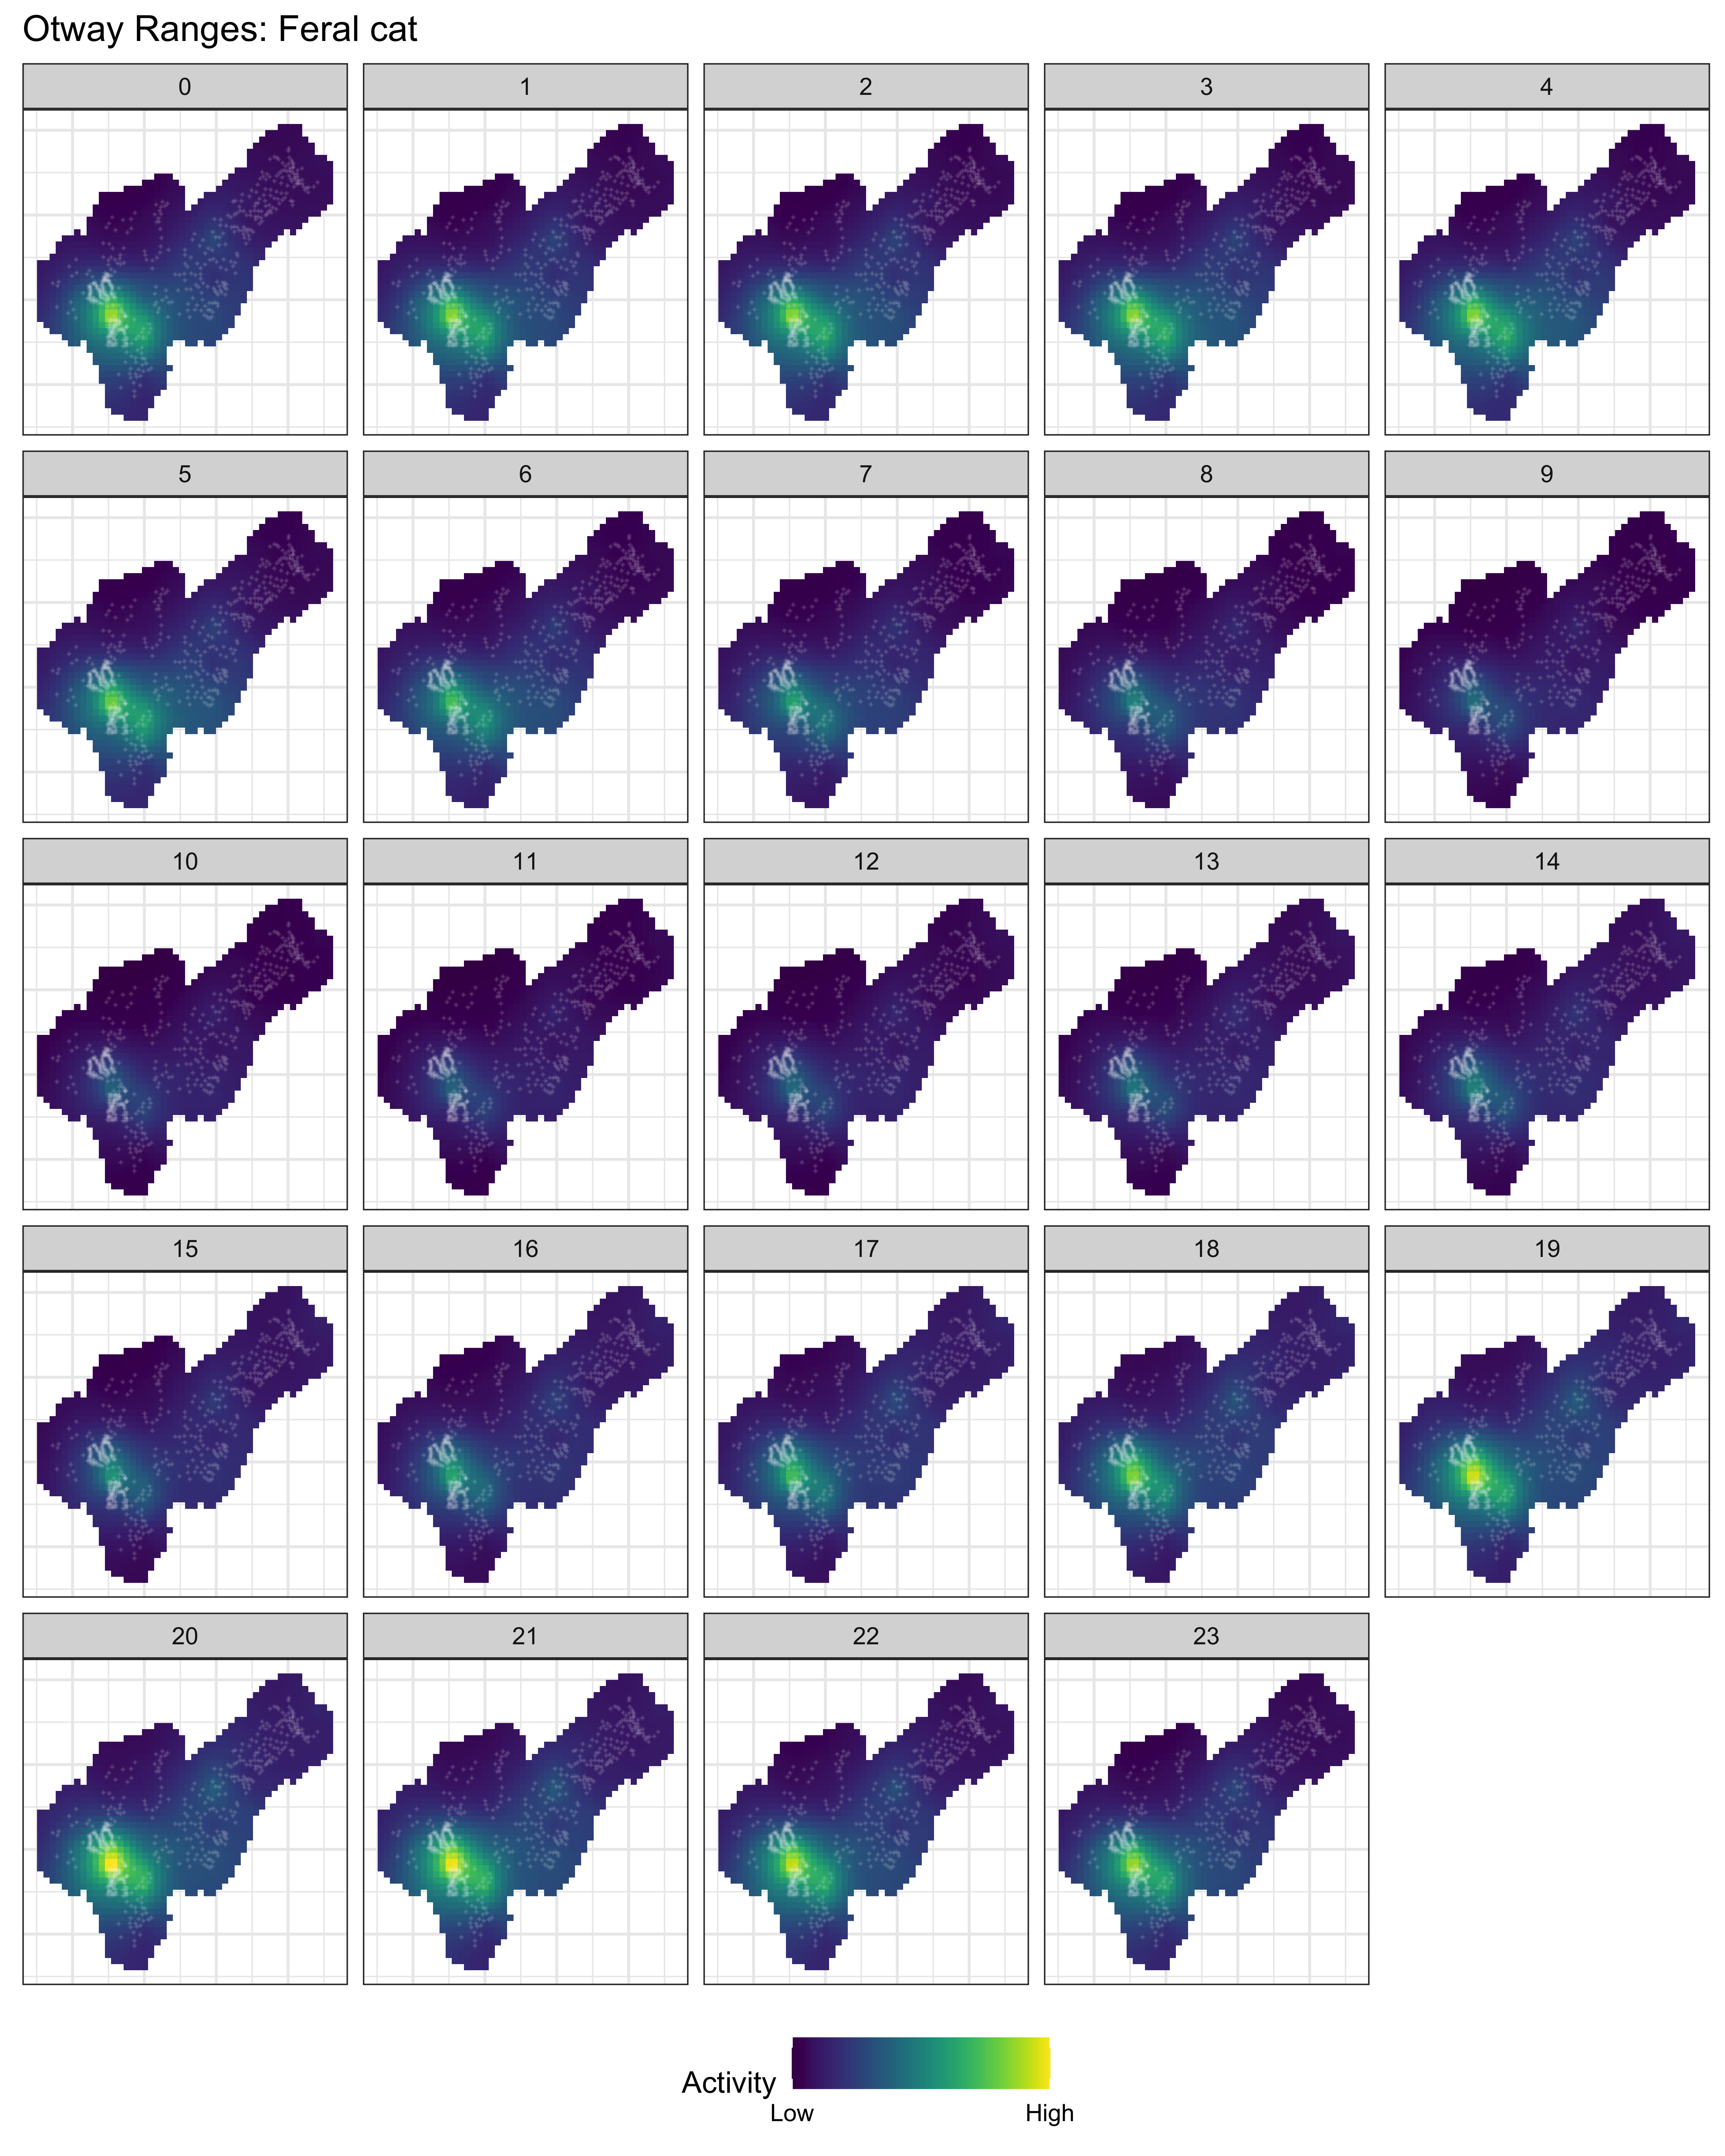
\includegraphics[width=1\linewidth]{../figs/spte_facet_o_cat} 

}

\caption{Overall spatial activity of feral cats \textit{Felis catus} for each hour of the day (0 - 23) in the Otway Ranges, Australia (model 1). White crosses depict unique camera-trap sites}\label{fig:diel-space-o-cat}
\end{figure}


\end{document}

